\documentclass[11pt,a4paper]{article}
\usepackage[T1]{fontenc}
\usepackage[utf8]{inputenc}
\usepackage{lmodern}
\usepackage[margin=30mm]{geometry}
\usepackage{microtype}
\usepackage{amsmath,amssymb,amsthm,mathtools}
\usepackage{enumitem}
\usepackage{graphicx}
\usepackage{tikz}
\usetikzlibrary{arrows.meta,calc,patterns}
\usepackage{xcolor}
\usepackage[colorlinks=true,linkcolor=blue!45!black,citecolor=blue!45!black,urlcolor=blue!45!black]{hyperref}
\hypersetup{pdftitle={The critical logarithmic correction for the planar XY model},pdfauthor={OpenAI}}

\newtheorem{theorem}{Theorem}[section]
\newtheorem{proposition}[theorem]{Proposition}
\newtheorem{lemma}[theorem]{Lemma}
\newtheorem{corollary}[theorem]{Corollary}
\theoremstyle{definition}
\newtheorem{definition}[theorem]{Definition}
\newtheorem{remark}[theorem]{Remark}

\newcommand{\R}{\mathbb R}
\newcommand{\Z}{\mathbb Z}
\newcommand{\T}{\mathbb T}
\newcommand{\E}{\mathbb E}
\newcommand{\Prob}{\mathbb P}
\newcommand{\cZ}{\mathcal Z}
\newcommand{\cR}{\mathcal R}
\newcommand{\cB}{\mathcal B}
\newcommand{\cE}{\mathcal E}
\newcommand{\norm}[1]{\lVert #1\rVert}
\newcommand{\abs}[1]{\lvert #1\rvert}
\newcommand{\ip}[2]{\langle #1,#2\rangle}
\newcommand{\dd}{\,\mathrm d}
\DeclareMathOperator{\Var}{Var}
\DeclareMathOperator{\Cov}{Cov}
\DeclareMathOperator{\dist}{dist}
\DeclareMathOperator{\supp}{supp}
\DeclareMathOperator{\tr}{tr}
\DeclareMathOperator{\Comp}{Comp}
\allowdisplaybreaks[2]
\setlist[enumerate]{label=\textup{(\roman*)},leftmargin=*}

\title{The critical logarithmic correction\\for the planar XY model}
\author{OpenAI}
\date{October 5, 2026}

\begin{document}
\maketitle
\begin{abstract}
We prove the critical logarithmic correction for the nearest-neighbor cosine
XY model on the square lattice. Let \(C_{b_c}(r)\) be the two-point correlation
at critical inverse temperature, obtained by taking the free-box thermodynamic
limit while the two sites remain \(r\) lattice steps apart along a coordinate
axis. Then
\[
C_{b_c}(r)=B_{\mathrm{XY}}r^{-1/4}(\log r)^{1/8}(1+o(1)),
\qquad B_{\mathrm{XY}}\in(0,\infty),
\]
as \(r\to\infty\).
\end{abstract}

\section{Introduction}\label{sec:introduction}

For an integer \(R\ge1\), let
\[
 \Lambda_R=[-R,R]^2\cap\Z^2,\qquad
 E_R=\{\{x,y\}\subset\Lambda_R:\abs{x-y}=1\}.
\]
The planar XY model at inverse temperature \(b>0\), with free boundary,
is the probability measure
\begin{equation}\label{eq:xy-law}
 \frac{1}{Z_{R,b}}
 \exp\left\{b\sum_{\{x,y\}\in E_R}\cos(\theta_x-\theta_y)\right\}
 \prod_{x\in\Lambda_R}\frac{\dd\theta_x}{2\pi},
 \qquad \theta_x\in\R/(2\pi\Z).
\end{equation}
Each unordered edge is counted once, and there are no exterior edges.
Write \(\E^{\rm free}_{R,b}\) for expectation.  For \(r\in\Z_{>0}\), with
\(e_1=(1,0)\), set
\begin{equation}\label{eq:critical-definition}
 \begin{split}
 C_b(r)&=\lim_{\substack{R\to\infty\\R\ge r}}
       \E^{\rm free}_{R,b}\cos(\theta_0-\theta_{re_1}),\\
 m(b)&=\lim_{r\to\infty}-\frac1r\log C_b(r),\qquad
 b_c=\inf\{b>0:m(b)=0\}.
 \end{split}
\end{equation}
The limits exist, \(0<b_c<\infty\), and \(m(b_c)=0\); see
\cite[Section~1.1 and Proposition~1.2]{C}.  The thermodynamic limit in the
first line is always taken before the separation tends to infinity.

\begin{theorem}\label{thm:main}
There is a constant \(B_{\rm XY}\in(0,\infty)\) such that
\[
 C_{b_c}(r)
 =B_{\rm XY}\,r^{-1/4}(\log r)^{1/8}(1+o(1))
 \qquad(r\to\infty,\ r\in\Z).
\]
\end{theorem}

The power \(r^{-1/4}\) is the critical decay rate.  The logarithm is
smaller than every fixed power of \(r\), but it prevents
\(r^{1/4}C_{b_c}(r)\) from converging to a finite nonzero limit.  The
theorem establishes this correction and the existence of a positive
finite microscopic amplitude for the free-box thermodynamic correlation.

\subsection{Background and relation to earlier work}

Berezinskii's spin-wave analysis predicted algebraic correlations for
planar spins at low temperature \cite{Berez1971}.  Kosterlitz and
Thouless described a transition driven by the unbinding of vortex
pairs \cite{KT1973}, and Kosterlitz developed a renormalization-group
analysis of the critical behavior of the nearest-neighbor model
\cite{Kosterlitz1974}.  For the Villain formulation, Janke records the
critical prediction, up to a multiplicative constant, as
\[
 |x|^{-1/4}(\log|x|)^{1/8}
 \left(1+O\left(\frac{\log\log|x|}{\log|x|}\right)\right);
\]
see \cite[Section~II, Equations~(2)--(3)]{Janke1997}.
Theorem~\ref{thm:main} establishes the leading equivalent, with a relative
\(o(1)\) error, for the ordinary cosine interaction and the free-box
thermodynamic correlation in Equation~\eqref{eq:critical-definition}.

Rigorous work established the phase picture through correlation
bounds and dual representations.  McBryan and Spencer proved
power-law upper bounds for two-dimensional planar-spin correlations
\cite{McBryanSpencer1977}.  Fr\"ohlich and Spencer proved a
low-temperature algebraic regime for the plane rotator and Villain
models through a multiscale Coulomb-gas analysis
\cite[Theorem~C]{FrohlichSpencer1981}.  For the cosine XY model,
van Engelenburg and Lis proved exponential decay below a threshold
and the lower bound \(1/(8|x-y|)\) at and above that threshold in
the limit over free boxes \cite[Theorem~1]{vanEngelenburgLis2023}.
These results include sharp information about the phases, while their
stated bounds do not determine the critical equivalent.

The dual height field provides another route to the transition.
Aizenman, Harel, Peled, and Shapiro related height depinning to
nonsummable spin correlations, including the Bessel height interaction
dual to the cosine XY model \cite{AHPS2022}.  Lammers identified an
exact relation between the XY and dual-height correlation lengths
\cite[Theorem~1]{Lammers2023}, and proved a localization dichotomy
with a universal positive lower bound on logarithmic height
fluctuations in the delocalized phase \cite{Lammers2026}.
These results constrain the transition through height information.

The lattice-Gaussian inequality of Regev and Stephens-Davidowitz
\cite{RSD2017} underlies the finite comparisons developed in
\cite[Section~2]{B} and passed to Bessel weights in \cite[Lemma~2.2]{C}.  In a related approach,
Aizenman, Harel, Peled, and Shapiro extended sublattice monotonicity of
height moment-generating functions to annealed Gaussian interactions;
their application to the XY dual uses a representation credited there
to Raoufi \cite[Lemma~9.6, Section~10.1, and Appendix~D]{AHPS2022}.
Bauerschmidt developed finite-range decompositions of Gaussian
fields using functional calculus \cite{Bauerschmidt2013}.
Bauerschmidt, Park, and Rodriguez obtained Gaussian scaling limits
for discrete Gaussian heights at high temperature
\cite{BPR2024I,BPR2024II}.  Falco's critical Coulomb-gas analysis gives
a rigorous example in which a marginal recursion produces a power law
with a multiplicative logarithm \cite{Falco2013}.  Its fractional
electric-charge observable is different from the magnetic XY insertion
considered here.

Theorem~\ref{thm:main} sharpens the companion result
\(C_{b_c}(r)=r^{-1/4+o(1)}\) of \cite{C}.  We use from that paper
the critical height coefficient \(a(b_c)=8\pi\), finite Bessel
comparisons, fixed-geometry and conditional height limits, and a
four-face characteristic estimate.  The analytic local maps come from
\cite{B}, and the sector costs for fixed positive holes and annular kernel
estimates from \cite{S}.  The annular argument is adapted to the pinned
rim below.  The cutoff initialization, quantitative coefficient estimate,
comparison of different starting histories, and extraction of the amplitude
are proved here.

\subsection{The route to the amplitude}

Fourier expansion of the spin interactions represents a correlation
as a ratio of partition functions for integer-valued heights on the
dual lattice.  The numerator shifts the height increments by a connection
whose circulation records the spin insertion.  This magnetic insertion
is not determined by convergence of height averages alone.

For an integer \(n\ge1\), let
\begin{equation}\label{eq:center-definition}
 M_n=\E^0_{n,b_c}\cos\theta_0,
\end{equation}
where \(\E^0_{n,b_c}\) denotes expectation for the measure obtained
from Equation~\eqref{eq:xy-law} on \(\Lambda_n\) by fixing all boundary
angles at zero and integrating only the interior angles.  The geometric
argument proves two comparisons:
\[
 \begin{aligned}
 \frac{M_{n'}}{M_n}&\longrightarrow d^{-1/8}
 &&\text{if }n,n'\to\infty\text{ and }n'/n\to d\in(0,\infty),\\
 \frac{C_{b_c}(r)}{M_r^2}&\longrightarrow c_{\rm shape}\in(0,\infty)
 &&\text{as }r\to\infty.
 \end{aligned}
\]
Annular interfaces separate the microscopic insertions from an exterior
with holes kept at fixed positive radius.  The sector and annular-kernel
estimates of \cite{S} control these interfaces, and the common microscopic
factors cancel in the comparisons.  A pinned-rim argument relates the
two-insertion calculation to the free-box thermodynamic correlation.
The first comparison gives \(M_n=n^{-1/8+o(1)}\), which will make the
cutoff loss negligible relative to the center observable, and later
extends an asymptotic from geometric sizes to all integers.  The second
reduces the theorem to a center asymptotic.

To compute \(M_n\), we cut off differences of noisy cell averages,
choosing the cell size according to the target square.  For the squares
used in the analytic comparison, the rough center bound makes this change
negligible in the center partition ratio.  After averaging to the associated
starting scale, the bulk interaction is small.  For the center insertion,
every expansion term carries one labelled component that retains the source
and its attached dependencies.  The norm of the resulting labelled activity
may grow polynomially with the cell size; a linear propagation estimate
controls it.

Let \(L>1\) be the fixed dyadic block ratio and \(j\) the absolute scale index.
After separating the Gaussian reference with height coefficient \(a=8\pi\),
the smoothed bulk interaction at block side \(L^j\) retains \(t_j/2\) times
the allocated gradient energy and a fundamental periodic term; the linear
part of the remaining activity's evolution contracts.  Coordinates adapted
to the pure Gaussian curve remove its drift and give a gradient coordinate
\(u_j\) and a signed fundamental Fourier coordinate \(Z_j\).  Their leading
recursion is
\[
 u_{j+1}-u_j\simeq-HZ_j^2,\qquad
 Z_{j+1}-Z_j\simeq-2(\log L)u_jZ_j,\qquad H>0.
\]
Physical torus variance and phase tests keep each finite history near the
Gaussian curve.  A phase lower bound derived from the four-face estimate
of \cite{C} prevents the fundamental direction from disappearing.
Comparing histories through the same finite physical torus tests controls
changes of starting scale without a rate for the height scaling limit.
Together with the recursion, these constraints yield the critical balance
\(HZ_j^2\sim2(\log L)u_j^2\), which gives harmonic decay of \(u_j\).
On the controlled interior ranges of the size-dependent histories used in
the comparison, the coordinate changes give \(t_j=u_j+O(j^{-2})\).  The
resulting estimate, uniform on each fixed such range, is
\[
 t_j=\frac{1}{2(\log L)j}
       +O\left(\frac{\log j}{j^2}\right).
\]

Let \(g_n\) be the minimum squared edge norm of a connection with the
\(2\pi\) circulation of one insertion in the corresponding dual square.
For \(n_0=L^N\) and \(n_1=L^{N+1}\), we use the same entry and a common
stop \(j'=N-O(\log N)\), leaving a number of terminal blocks that grows
as a small power of \(N\).  We choose the field-independent factors removed
at each step so that their complete contributions to the insertion ratio
agree between sizes.  The source term remaining at the stop is controlled
relative to the source coefficient already extracted.  Integration of the
common phase then removes the linear periodic term, and a comparison of the
terminal Gaussian fields leaves the gradient contribution with a summable
error:
\[
 \log\frac{M_{n_1}}{M_{n_0}}
 =-\frac{1-t_{j'}}{2a}\bigl(g_{n_1}-g_{n_0}\bigr)+\epsilon_N,
 \qquad \sum_N|\epsilon_N|<\infty.
\]
Here \(g_{L^N}=2\pi(\log L)N+c_N\) with \(c_N\) convergent.  Substitution
of the trajectory estimate gives the constant increment \(-(\log L)/8\)
and the correction \(1/(16N)\).  The unweighted Green differences
\(c_{N+1}-c_N\) telescope, and summation by parts treats the differences
weighted by \(1/N\); the other errors are absolutely summable.  Summation
therefore gives a positive finite center amplitude with logarithmic power
\(1/16\).  The first geometric comparison extends this equivalent to all
integer sizes, and the bulk comparison squares the logarithmic power to
\(1/8\).

\section{Height representation and critical inputs}\label{sec:heights}

We first pass from spins to Bessel heights, fixing the normalization
and the boundary conventions.  We then record the finite comparisons
and critical height limits used in the geometric and analytic arguments.
These inputs concern the Bessel weights obtained from the XY model.

\subsection{Dual partition functions}

Choose one orientation of each edge of a finite nearest-neighbor
graph \(G=(V,E)\) and put \(\nabla_eh=h_y-h_x\) for \(e=(x,y)\).
We call these height vertices and edges \emph{primary}, to distinguish
them from the auxiliary subdivisions in the comparison proof;
\emph{primal} refers to the spin lattice.
The height takes values in \(2\pi\Z\).  Its increment weight is
\begin{equation}\label{eq:bessel-weight}
 p_b(j)=e^{-b}I_j(b),\qquad
 \sum_{j\in\Z}p_b(j)e^{tj}=\exp\{b(\cosh t-1)\}.
\end{equation}
Here \(I_j\) is the modified Bessel function.  Thus \(p_b\) is the law
of the difference of two independent Poisson variables of mean \(b/2\).
An \emph{integral connection} is an antisymmetric edge function
\(\tau:E\to2\pi\Z\).  The weight in that sector is
\[
 \prod_{e\in E}p_b\left(\frac{\nabla_eh+\tau_e}{2\pi}\right).
\]
A connection is flat where its circulation around every contractible
cycle is zero.
Its circulations around the remaining holes are its periods.

We allow nonnegative quadratic penalties in real linear observations,
hard pins, and prescribed relative height data.  Every observation
used after a cut is supported in one component.  A component with no
absolute constraint or confining observation is summed modulo a common
translation by \(2\pi\Z\); when its constant is confined, all its
translation copies are summed.  A hard pin fixes that constant instead.
Relative translations between cut components are summed again on
restoration.  Write \(Z_G^\tau\) for a partition function with these
conventions and \(Z_G^0\) for the same graph, cuts, and penalties with
all affine data centered.

An integral gauge change replaces \(\tau\) by \(\tau+\nabla\psi\) and
the height variable by \(h-\psi\), where \(\psi:V\to2\pi\Z\).
This is an exact reindexing when every affine datum is changed with
the height.  A penalty \(\|Bh-y\|^2/2\) then has center \(y-B\psi\),
and absolute data \(b^p\) on a set \(p\) become \(b^p-\psi|_p\).
For relative data \(h_z-h_{z_0}=u_z\), the new value is
\(u_z-\psi_z+\psi_{z_0}\).  Thus a hard zero pin is preserved when
\(\psi=0\) on it, and a constraint requiring all heights on a set
to be equal is preserved when \(\psi\) is constant there.

\begin{lemma}[Spin--height duality]\label{lem:duality}
In a free spin box, the two-point correlation is \(Z_G^\tau/Z_G^0\)
on the dual graph with the exterior face fixed at height zero.
One may represent that face by separate exterior incident copies, all
pinned at zero, or identify those copies while retaining every edge.
Circulations below are read in the dual with the exterior copies identified.
The connection has circulations \(+2\pi\) and \(-2\pi\) around the
two sources and can be supported on the dual bonds crossing a primal
current path joining them.

The center magnetization \(M_n\) defined in
\eqref{eq:center-definition} satisfies
\(M_n=\E_{n,b_c}^{\,0}e^{i\theta_0}>0\).
It is \(Z_G^\tau/Z_G^0\) on the free dual square with
\(2n\) dual vertices on each side, indexed by the primal cells, where
\(\tau\) has one circulation \(2\pi\) around the center.  It may be
supported on the dual bonds crossing a primal current path from the
center to the boundary.
\end{lemma}

\begin{proof}
Expand each spin interaction in its Fourier series,
\[
 e^{b\cos(\theta_x-\theta_y)}
 =\sum_{j\in\Z}I_j(b)e^{ij(\theta_x-\theta_y)}.
\]
In the fixed-boundary square first cancel the interactions whose two
endpoints are fixed boundary spins.  Integrating each remaining
unfixed spin imposes its integer divergence condition.  Subtract a
fixed primal current carrying the inserted charges along the stated
path.  The remaining current is divergence free at every integrated
vertex: at all vertices in the free spin box and at the interior
vertices in the fixed-boundary square.  Rotation onto dual edges then
gives an integral gradient.  In the free spin box its exterior height
is fixed; in the fixed-boundary square it is determined modulo a common
translation.  The factors \(e^b\) in \eqref{eq:bessel-weight} cancel
in the ratio.  The numerator and denominator are sums of strictly
positive Bessel weights, so the ratios are positive.  Current reversal
identifies each insertion with its conjugate, giving the stated real
cosine expectations.  This is the duality of \cite[Lemma~2.1]{C} and
\cite[Lemma~2.1]{S}, with their respective boundary conventions.
For the classical current and Bessel-height representations, see also
\cite[Appendix~A]{FrohlichSpencer1981} and
\cite[Section~2]{vanEngelenburgLis2023}.
\end{proof}

The reference form on a retained primary graph is the unit-conductance
form
\begin{equation}\label{eq:reference-energy}
 \ip{g}{A_Gg}=\sum_{\{x,y\}\in E}(g_x-g_y)^2.
\end{equation}
It converges under lattice scaling to \(\int|\nabla g|^2\).
For the four nearest steps this is exactly the operator \(A_0\) in
\cite{B}.  We write \(A\) when the graph is understood.

\subsection{The critical height inputs}

\begin{proposition}[Finite affine comparisons]\label{prop:comparisons}
On every fixed primary graph, the Bessel height law has the following
properties.
\begin{enumerate}
\item A shifted-to-centered partition ratio is at most one and
decreases when the same nonnegative quadratic precision is added to
the affine and centered coordinates.  Affine data may include an
integral connection, observation centers, and compatible nonzero
equality values.  The monotonicity remains valid with a fixed real
linear statistic in the numerator exponent, although the tilted
ratio need not be at most one.
\item For zero affine data, centered covariances and centered real moment generating
functions decrease under added centered precision.  Centered
characteristic coefficients allowed by the constant convention in both
laws are nonnegative and increase under added precision.  They are
strictly positive for the finite-graph phases
used below, whose coefficient total on every unconfined component is
an integer.
\item If \(X=\sum_e q_e\nabla_eh\) in a centered law, then
\[
 \Var X\le C_b\sum_eq_e^2,\qquad
 \E|X|^k\le C_{k,b}\left(\sum_eq_e^2\right)^{k/2}.
\]
More generally, after releasing endpoint, curl, and period constraints
while retaining independent primary increments, a tilt with
\(\max_e|q_e|\le K\) costs at most
\(\exp(C_{b,K}\sum_eq_e^2)\).
\end{enumerate}
The statements include independent Gaussian observation noises.
Released constants are taken modulo translations or confined; a real
statistic used in releasing a constant must annihilate it.
\end{proposition}

\begin{proof}
The comparison assertions are \cite[Lemma~2.2]{C}.  That lemma replaces
each primary bond by a chain of lattice-Gaussian bonds, applies the
finite affine comparison on the enlarged lattice, and passes to the
limit at the fixed primary graph.  Equality constraints are limits
of positive quadratic penalties.  Thus the same affine statistic is
kept when observations or constraints are released.
Strict positivity for the phases used here follows from the
phase-transfer estimate \cite[Equation~(2.2) and its proof]{C}: on an
unconfined component subtract an integer point charge and interpolate
the remaining zero-total finite-variance test from zero; on a confined
component interpolate directly using its finite fixed-graph variance.
The finite lattice-Gaussian comparison underlying this argument is
developed in \cite[Lemma~2.1]{B} from the inequality of
\cite[Theorem~2.1 in the arXiv version]{RSD2017}.

For the last assertion, perform these releases before estimating the
tilt.  The independent primary transform is the product of the
transforms in \eqref{eq:bessel-weight}, with \(t=2\pi q_e\).
For \(|q_e|\le K\),
\(\cosh(2\pi q_e)-1\le C_Kq_e^2\).  This gives the last bound.
Normalize \(q\) by \((\sum q_e^2)^{1/2}\) and differentiate bounded
exponential moments to obtain the stated moment bounds.  These are
the primary reference-cost bounds of \cite[Lemma~2.3]{C}; no bound
on the microscopic Gaussian precision of the subdivided chains is
used.
\end{proof}

The next proposition uses absolute pin data: \(h_H=0\) fixes every
primary height in \(H\), and \(b^p\) specifies a compatible absolute
height at every primary vertex of \(p\).  Its approximation by finite
guard observations is understood in probability, at each prescribed
tolerance, under the sampled law stated there.  The finite list of
smooth guard probes is fixed before the lattice limit and enlarged
afterward to reduce the tolerance.

\begin{proposition}[Critical coefficient and mixed limits]\label{prop:height-inputs}
For the critical parameter in \eqref{eq:critical-definition}, the
Bessel height coefficient of \cite{C} is
\begin{equation}\label{eq:critical-coefficient}
                         a=a(b_c)=8\pi.
\end{equation}
At this parameter the following fixed-geometry statements hold.
\begin{enumerate}
\item Let the fixed geometry belong to the polygonal Lipschitz class
of \cite[Theorem~3.1]{C}: it is a finite union of bounded rectangular
pieces with nondegenerate faces and widths.  Pieces in one component
are joined along full interfaces, which may be subdivided into segments;
point contacts do not join components.  All passages have positive width.
Allow free walls and
hard pins on the primary vertices in aligned unions of positive-area
boxes.  On each component
\(U\), fixed bounded, piecewise continuous density smears of the height
have Gaussian Laplace and moment limits
with covariance the inverse of
\[
 a^{-1}\int_U|\nabla v|^2
 \quad\text{on}\quad
 \{v\in H^1(U):v=0\text{ on the pin}\}.
\]
For an unpinned component this is a statement about mean-free smears;
its fractional mean modulo \(2\pi\) becomes independent and uniform.
Fixed finite-rank nonnegative penalties in box averages give the
corresponding Gaussian laws, with constants integrated when the
penalties confine them.  The statements hold along every admissible
mesh sequence, including bounded rounding of the fixed geometry.
They include energy-approximable shifts in the sense of
\cite[Theorem~3.1]{C}.
\item Start with no hard pins and use the centered law whose
component-local box-average penalties confine every pre-pin component
constant.  Let \(H,p\) be positively separated unions of boxes.  Put
\[
 D(H,p)=\log\frac{\Prob(h_H=0\mid h_p=0)}{\Prob(h_H=0)},\qquad
 r_H(b^p)=\frac{\Prob(h_H=0\mid h_p=b^p)}
                 {\Prob(h_H=0\mid h_p=0)}.
\]
Then \(D(H,p)\ge0\) converges to the Gaussian pin interaction,
\(0<r_H\le1\), and
\(\E_{\mathrm{cen}} r_H=e^{-D(H,p)}\), where the expectation samples
the guard data in the centered law.
For every fixed finite list of these density smears and box averages,
the conditional Laplace transforms and \(r_H\) admit approximations
by fixed finite lists of smooth observations of the guard data, whose
laws and functions converge to their Gaussian counterparts.  The
list is enlarged after the lattice limit.  These convergence assertions
also hold when the data are sampled under a fixed finite real linear
tilt; \(D\) and \(r_H\) retain their centered definitions above.
\end{enumerate}
\end{proposition}

\begin{proof}
Equation~\eqref{eq:critical-coefficient} is the conclusion of
\cite[Section~6]{C}.  The first and second parts are respectively
\cite[Theorems~3.1 and~3.2]{C}.  In the second part, observations are
component-local before pins are imposed.  The finite-observation
formulation is part of the theorem; it does not assert uniform
convergence at every microscopic guard value.
\end{proof}

We also use the restoration consequence \cite[Lemma~3.9]{C}.
Suppose every endpoint of a restored bond, and the support of every
restored form, lies in a core \(H\) separated from a guard \(p\).
If \(r_\Delta\) is the conditional restoration factor divided by
its value at zero guard data, then \(r_H\le r_\Delta\le1\).
The guard laws in the two topologies transfer events whose
probabilities tend to zero in either direction, also under a fixed
real linear tilt.  The finite-observation approximations above concern
conditional Laplace transforms and \(r_H\); no additional limit for
\(r_\Delta\) is asserted.  In each use, the graph, pin regions, and
observation cells are fixed before the lattice limit.

\section{Fixed-geometry comparison}\label{sec:geometry}

The center magnetization isolates the microscopic cost of one spin
insertion.  We compare boxes by placing the same finite nest of annuli
around each corresponding source.  An attachment calculation separates
the ratio of a nest from that of its exterior; the nest ratios then
cancel, leaving exterior energies at fixed geometry.  The first comparison
is between square sizes, and the second concerns the free-box thermodynamic
correlation of two insertions.  All continuum limits used here keep the
holes and every separating region at fixed positive size.

\begin{proposition}[Comparison with center magnetization]
\label{geo:comparison}
For integer sequences \(n,n'\to\infty\) with \(n'/n\to d\in(0,\infty)\),
\begin{equation}\label{geo:center-ratio}
                  \frac{M_{n'}}{M_n}\longrightarrow d^{-1/8}.
\end{equation}
There is a constant \(c_{\rm shape}\in(0,\infty)\) such that
\begin{equation}\label{geo:bulk-ratio}
                  \frac{C_{b_c}(r)}{M_r^2}\longrightarrow c_{\rm shape}
                  \qquad(r\to\infty,\ r\in\Z).
\end{equation}
Here \(C_{b_c}\) is the thermodynamic limit in
\eqref{eq:critical-definition}; that limit precedes \(r\to\infty\).
In particular, \(M_n=n^{-1/8+o(1)}\).
\end{proposition}

\subsection{Separating the insertion from the exterior}

For a graph with the boundary and constant conventions of
Section~\ref{sec:heights}, write
\(\Phi_G^\tau=Z_G^\tau/Z_G^0\) for its bare sector ratio.
The fixed-domain sector input evaluates this ratio on a free exterior.
Let \(U\) be a bounded connected rectilinear domain with a simple outer
boundary and finitely many disjoint simple holes, all with dyadic vertices,
positive side lengths, and positive passages.  Give the height graph
free walls.  If \(\vartheta_0\) is a smooth closed one-form near
\(\overline U\) whose periods about the holes are prescribed multiples
of \(2\pi\), set
\[
 \mathcal M_U(\vartheta_0)
   =\inf_{g\in H^1(U)}\int_U|\vartheta_0+\nabla g|^2.
\]
Let \(\mathcal G_\nu(U)\) be its nearest-neighbor primary graph at mesh
\(\nu^{-1}\).  For integral lattice connections that are flat on the
retained graph away from the holes and have these periods,
the sector theorem of \cite[Theorem~3.1]{S} states that
\begin{equation}\label{geo:free-sector}
 \Phi_{\mathcal G_\nu(U)}^\tau
       \longrightarrow \exp\{-\mathcal M_U(\vartheta_0)/(2a)\}
       \qquad(\nu\to\infty),
\end{equation}
where \(a=8\pi\).  The limit holds along
every coherent bounded-step rounding of this fixed geometry.  The
energy depends only on the periods.  This statement concerns free
height walls; a pinned exterior will be treated below.

To connect \eqref{geo:free-sector} to a microscopic source, use the
annular construction of \cite[Sections~4 and~5]{S}.  Fix a small
\(\varepsilon>0\) and a rectilinear disk \(P\) with dyadic vertices
such that
\begin{equation}\label{geo:polygon}
 B(0,1-\varepsilon)\subset P\subset B(0,1+\varepsilon).
\end{equation}
Choose a sufficiently large power of four \(\lambda\), and an integer
\(\varrho_0\) aligned so that all relevant array divisions lie between
rows of dual vertices.  Put \(\varrho_i=\varrho_0\lambda^i\).
The \(i\)-th annulus has walls \(\varrho_{i-1}P\) and
\(\varrho_iP\).  Write \(Q_s=(-s,s)^2\) and
\(A_\lambda=\lambda P\setminus P^\circ\).  In the reference annulus
\(A_\lambda\), the guard is
\(\overline{Q_{2\sqrt\lambda}}\setminus Q_{\sqrt\lambda}\), and the
inner and outer end regions are \(A_\lambda\cap\overline{Q_4}\) and
\(A_\lambda\setminus Q_{\lambda/4}\), respectively.  Scale these
three regions by \(\varrho_{i-1}\), and call the guard \(\mathsf P_i\).
It is a full separating band, and each end contains every endpoint
in that annulus of a bond to be restored at its wall.  These prescribed
bands, with positive gaps, are the geometry used in the flat-pin
estimate below.

Choose one vertex in \(\mathsf P_i\).  A guard datum records every
height difference from that vertex.  In the annular quotient choose
its height to be zero, so the datum specifies every guard height.
The nearest-neighbor weight then factors between the two sides
conditionally on that datum.  Write \(\mu_i^\tau\) for the guard law
in the cut annulus, with its one common constant quotiented out.

A core is a connected finite block filling the first hole; it may
carry the source and has no guard data.
At an interface in this construction, let \(T^\tau(u)\) be the restored
partition sum divided by the cut partition sum at its incident guard
data \(u\),
and put \(d_T=T^0(0)\).  The restored sum includes the relative
integer translations of the joined components.  The same definition
applies to one joint interface joining several last annuli to a
connected exterior, with no direct bonds between distinct incident
annuli.  Its data are those in the incident annuli, while all exterior
heights are summed together inside that one kernel.
For a vertex region \(H\), let \([H]\) denote the event that all its
heights are equal, without prescribing their common value.  In a
centered cut annulus with guard \(\mathsf P_i\), put
\[
 \overline D_i(H,\mathsf P_i)
   =\log\frac{\Prob([H]\mid[\mathsf P_i])}{\Prob([H])}.
\]
The upper kernel bound of \cite[Lemma~5.1]{S}, its Equation~(8), holds
for all these interfaces, including a core interface.  For an
annulus--annulus or joint exterior interface, its Equation~(9) also
gives the centered average bound:
\begin{equation}\label{geo:kernel-bounds}
 0<\frac{T^\tau(u)}{d_T}\le1,
 \qquad
 \int\frac{T^0}{d_T}\prod_i\dd\mu_i^0
       \ge \exp\left\{-\sum_i\overline D_i(H_i,\mathsf P_i)\right\}.
\end{equation}
The sum and product use the incident annuli and the appropriate end
in each.  The first bound is pointwise in the data, and the second
is an average under independent centered cut annuli.  The centered
divisor \(d_T\) therefore works for the shifted kernel as well.
The flat-pin estimate of \cite[Proposition~4.1]{S}
makes each interaction on the right arbitrarily small in the mesh
limit by taking \(\lambda\) large at fixed \(P\).

Two consequences of \cite[Proposition~5.3 and Corollary~5.5]{S}
control how the averaged loss passes through a whole nest.
For any \(\xi\in(0,1/64)\), one can first take
\(\varepsilon\) small, then \(\lambda\) large, and finally the fixed
aligned threshold \(\varrho_0\) large, so that every interface between
successive annuli of these radii satisfies
\begin{equation}\label{geo:regular-loss}
 \int\left(1-\frac{T_i^\tau}{d_{T_i}}\right)
             \dd(\mu_i^\tau\otimes\mu_{i+1}^\tau)\le\xi.
\end{equation}
This holds in the centered sector and in either unit-period sector,
when restoration introduces no source.  It follows from the exact
sector identity (10) in that proposition and
\eqref{geo:free-sector}; it is the normalized estimate (11) there.
All late annuli obey the same bound because they refine the same
fixed geometry.  Fix one such core, containing the source in a unit
sector, and fix its connection once on the increasing family.  In a nest
of \(J\) annuli, the law of its last guard then has density at most \(2\)
with respect to
\(\mu_J^\tau\), for all sufficiently large \(J\).  This holds in
all three sectors and for identical lattice translates.  The only
lower assumption on the first core kernel is its strict positivity;
no uniform positive lower bound on that kernel is required.
This density bound compares the actual last-guard law, after all inner
blocks have been joined, with the cut law used in the averaged estimate.

It remains to attach the whole nests to their exterior.
Let \(\mathcal N_J\) be the bare sector ratio of one whole
free nest of depth \(J\), with its core and a unit source.  Integral
gauge changes and reversal of all heights show that the same
\(\mathcal N_J\) is obtained from any lattice translate and either
sign.  This is the common factor that will cancel in both comparisons.
Suppose \(k\) such nests, with disjoint closures, attach to a
connected exterior.  The graph of cut blocks, with an edge for each
interface, is a tree rooted at the exterior; there are no other block
adjacencies, in particular no direct bonds between distinct incident
last annuli.  Write \(\mu_{J,i}^\tau\) for the cut guard law in
the \(i\)-th incident last annulus, with its restricted connection.
In the following ratio, ``joined'' means the
exterior after joining only the \(k\) last annuli; the holes then have
the inner radii of those annuli.  Define
\begin{equation}\label{geo:joining-ratio}
 \mathfrak q^\tau_{\rm ext}
  =\frac{\Phi_{\rm joined}^\tau}
         {\Phi_{\rm ext}^\tau\prod_{i=1}^k\Phi_{{\rm last},i}^\tau}.
\end{equation}
Releasing those interfaces gives \(0<\mathfrak q^\tau_{\rm ext}\le1\).
Exact summation of the interface kernel, which is Equation~(10) of
\cite{S}, gives
\begin{equation}\label{geo:kernel-sector-identity}
 \int\frac{T^\tau_{\rm ext}}{d_{\rm ext}}
              \prod_i\dd\mu_{J,i}^\tau
 =\left(\int\frac{T^0_{\rm ext}}{d_{\rm ext}}
              \prod_i\dd\mu_{J,i}^0\right)\mathfrak q^\tau_{\rm ext}.
\end{equation}
Thus a sufficient attachment condition, along the lattice sequence
in question, is
\begin{equation}\label{geo:attachment-condition}
 \sum_i\overline D_i(H_i,\mathsf P_i)\le\delta+o(1),
 \qquad \log\mathfrak q^\tau_{\rm ext}\ge-\delta-o(1),
\end{equation}
with \(\delta>0\) arbitrarily small.  Indeed,
\eqref{geo:kernel-bounds} and \eqref{geo:kernel-sector-identity}
bound the shifted average loss by
\(1-e^{-2\delta-o(1)}\), and the centered one by
\(1-e^{-\delta-o(1)}\).  This estimate is averaged over the independent
cut-annulus laws, without any uniform lower bound at individual data.

The lower thermodynamic comparison below retains a hard pin in the
exterior.  We therefore check that the same reasoning applies when
that pin fixes the exterior constant and is kept in both the restored
and cut graphs.  The entire hard constraint remains in the exterior
partition sum and joint kernel; for the rim below, this includes every
equality \(h_x=0\) on the rim.  Accordingly,
\(d_{\rm ext}=T_{\rm ext}^0(0)\) is evaluated with that pin retained.
Prescribed relative guard data are affine equalities, so
Proposition~\ref{prop:comparisons}, with the independent increments
on cut bonds, still gives \(0<T^\tau/d_T\le1\).  To prove the centered
bound in \eqref{geo:kernel-bounds}, impose the flat end event \([H_i]\)
in each incident annulus and choose its representative to be zero on
that end.  The restored-bond factor now depends on the relative integer
translations and the exterior heights, and is independent of the
guard data.  Adding these end constraints decreases the data-to-zero
ratio, giving the product of the annular flat-pin ratios in
\eqref{geo:kernel-bounds}.  This proof uses no unpinned exterior law.
For multiplication, place the exterior, with its full pin constraint,
at the root of the tree of cut blocks.  Its configurations are summed
subject to every retained pin equality.  Once its additive constant is
fixed, the remaining block constants are in bijection with the integer
differences along the tree edges.  Conditioning on the full annular guards
separates their two sides, so the tree multiplication of
\cite[Lemma~5.2]{S} and the identity
\eqref{geo:kernel-sector-identity} follow with this pin retained.

To finish the attachment calculation, let \(e_\tau\) be the expectation
of \(T^\tau_{\rm ext}/d_{\rm ext}\) under the product of the propagated
last-guard laws of the whole nests, and define \(e_0\) in the same way.
Their densities relative to the independent cut laws are at most
\(2^k\), so \eqref{geo:attachment-condition} implies
\(1-e_\tau,1-e_0\le 2^k(1-e^{-2\delta-o(1)})\).
Exact multiplication and cancellation of \(d_{\rm ext}\) give
\begin{equation}\label{geo:attachment-factorization}
 \Phi_{\rm full}^\tau
       =\mathcal N_J^k\Phi_{\rm ext}^\tau\frac{e_\tau}{e_0},
 \qquad
 \log\Phi_{\rm full}^\tau
       =k\log\mathcal N_J+\log\Phi_{\rm ext}^\tau
                              +O_k(\delta)+o(1).
\end{equation}
Here \(\delta\) is small at fixed \(k\), and \(J\to\infty\) with
the core, \(P,\lambda,\varrho_0\) fixed.  The first identity is exact;
the second is the attachment consequence we shall use.

\subsection{A pinned comparison for the thermodynamic correlation}

We first place the desired thermodynamic correlation between two finite
height ratios.  For a large dyadic \(R_{\rm out}\ge8\), let
\[
 \mathsf F_{R_{\rm out}}
       =\overline{Q_{7R_{\rm out}/8}}\setminus Q_{3R_{\rm out}/4}.
\]
The region \(\mathsf F_{R_{\rm out}}\) is a positive-width rim, expressible as an
aligned union of positive-area boxes with dyadic vertices.  In lattice units let
\(G_{R_{\rm out},r}\) be the dual primary array in \(rQ_{R_{\rm out}}\), with coherent
rounding, and let \(\mathsf F_{R_{\rm out},r}\) be the filled primary boxes
representing \(r\mathsf F_{R_{\rm out}}\).  Put
\[
 \Phi_{R_{\rm out},r}^{\rm fr}=\Phi_{G_{R_{\rm out},r}}^\tau,
 \qquad
 \Phi_{R_{\rm out},r}^{\rm pin}
     =\Phi_{G_{R_{\rm out},r},\,h_{\mathsf F_{R_{\rm out},r}}=0}^\tau,
\]
where the sources are \(0,re_1\), with periods \(+2\pi,-2\pi\).

There is one connection suitable for both comparisons.  In the primal
lattice take the actual nearest-neighbor path
\[
 (0,0),(1,0),\ldots,(r,0)
\]
and give its edges the unit current directed from one source to the
other.  The dual connection is supported on the dual bonds crossing
these path edges.  They lie inside \(rQ_{R_{\rm out}/2}\), for all large \(r\),
so the connection vanishes on every bond meeting the rim or lying
outside it.  Use this connection in every larger free spin box.

For a box \(\Lambda_R\) containing \(rQ_{R_{\rm out}}\) in its interior, release
the matching equalities for all bonds crossing the boundary of
\(G_{R_{\rm out},r}\), retaining their independent Bessel increments as in the
finite comparison.  The resulting inner height component has a free
wall; the connection on the exterior component is zero and its ratio
cancels.  Proposition~\ref{prop:comparisons} therefore gives the upper
bound by \(\Phi_{R_{\rm out},r}^{\rm fr}\).  For the lower bound add the
common hard pin \(h_{\mathsf F_{R_{\rm out},r}}=0\) before making any cut.  Added precision
decreases the sector ratio.  This filled rim separates the interior
from the entire exterior.  Because the connection is supported on the
specified path inside the rim, the partition factor for all exterior
variables, including the original fixed exterior face, is identical in
the numerator and denominator.  It cancels.  The same cancellation of
the outer collar occurs in \(G_{R_{\rm out},r}\) with this rim pinned,
so the remaining ratio is exactly \(\Phi_{R_{\rm out},r}^{\rm pin}\).
Hence, for every sufficiently
large \(R\) at each fixed \(R_{\rm out},r\),
\[
 \Phi_{R_{\rm out},r}^{\rm pin}\le
 \E^{\rm free}_{R,b_c}\cos(\theta_0-\theta_{re_1})
 \le \Phi_{R_{\rm out},r}^{\rm fr}.
\]
Taking \(R\to\infty\) at this point proves
\begin{equation}\label{geo:thermodynamic-bracket}
 \Phi_{R_{\rm out},r}^{\rm pin}\le C_{b_c}(r)
                                    \le \Phi_{R_{\rm out},r}^{\rm fr}.
\end{equation}
The finite comparisons just used are the affine and matching-constraint
comparisons of \cite[Lemma~2.2]{C}; the exterior cancellation is why the
location of the connection matters.

Figure~\ref{geo:pinned-schematic} shows the separation used for the
pinned sector estimate.  In the later annular application, its two holes
are those left in the exterior when the two insertion nests are removed
from the full pinned comparator \(\Phi_{R_{\rm out},r}^{\rm pin}\).
Its retained arc \(\Gamma\) is the portion
of the primal source path between the two hole walls.  The guard
separates the strip bonds from the artificial side boundary of the patch,
including at the hole exits; the rim lies beyond the patch.

\begin{figure}[tb]
\centering
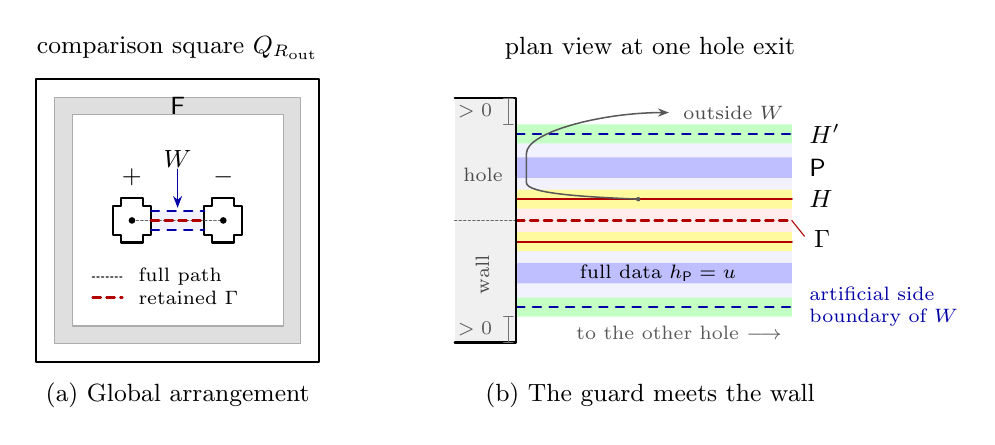
\begin{tikzpicture}[font=\small,line cap=round,line join=round]
  \begin{scope}
    \draw[thick] (-1.8,-1.8) rectangle (1.8,1.8);
    \path[fill=gray!25,even odd rule]
      (-1.56,-1.56) rectangle (1.56,1.56)
      (-1.34,-1.34) rectangle (1.34,1.34);
    \draw[gray!65] (-1.56,-1.56) rectangle (1.56,1.56);
    \draw[gray!65] (-1.34,-1.34) rectangle (1.34,1.34);
    \node at (0,1.45) {\(\mathsf F\)};
    \path[fill=blue!5] (-.34,-.12) rectangle (.34,.12);
    \foreach \x in {-.58,.58} {
      \begin{scope}[xshift=\x cm]
        \path[draw,fill=white,thick]
          (-.14,-.28)--(.14,-.28)--(.14,-.18)--(.24,-.18)
          --(.24,.18)--(.14,.18)--(.14,.28)--(-.14,.28)
          --(-.14,.18)--(-.24,.18)--(-.24,-.18)--(-.14,-.18)--cycle;
      \end{scope}
    }
    \draw[blue!65!black,dashed,thick]
      (-.34,.12)--(.34,.12) (-.34,-.12)--(.34,-.12);
    \draw[black!60,densely dotted,line width=.65pt] (-.58,0)--(.58,0);
    \draw[red!70!black,densely dashed,thick] (-.34,0)--(.34,0);
    \fill (-.58,0) circle (1.2pt) (.58,0) circle (1.2pt);
    \node[above] at (-.58,.31) {\(+\)};
    \node[above] at (.58,.31) {\(-\)};
    \node at (0,.78) {\(W\)};
    \draw[-{Stealth[length=1.5mm]},blue!65!black] (0,.65)--(0,.16);
    \draw[black!60,densely dotted,line width=.65pt] (-1.08,-.72)--(-.70,-.72);
    \node[anchor=west,font=\scriptsize] at (-.62,-.72) {full path};
    \draw[red!70!black,densely dashed,thick] (-1.08,-.98)--(-.70,-.98);
    \node[anchor=west,font=\scriptsize] at (-.62,-.98) {retained \(\Gamma\)};
    \node[above] at (0,1.92) {comparison square \(Q_{R_{\rm out}}\)};
    \node[below] at (0,-1.94) {(a) Global arrangement};
  \end{scope}

  \begin{scope}[xshift=4.3cm]
    \path[fill=gray!12] (-.78,-1.55) rectangle (0,1.55);
    \path[fill=blue!5] (0,-1.10) rectangle (3.50,1.10);
    \path[fill=red!7] (0,-.27) rectangle (3.50,.27);

    \path[fill=yellow!38]
      (0,.15) rectangle (3.50,.27) (0,.27) rectangle (3.50,.39)
      (0,-.39) rectangle (3.50,-.27) (0,-.27) rectangle (3.50,-.15);
    \path[fill=blue!25]
      (0,.54) rectangle (3.50,.80) (0,-.80) rectangle (3.50,-.54);
    \path[fill=green!23]
      (0,.98) rectangle (3.50,1.10) (0,1.10) rectangle (3.50,1.22)
      (0,-1.22) rectangle (3.50,-1.10) (0,-1.10) rectangle (3.50,-.98);

    \draw[blue!65!black,dashed,thick]
      (0,1.10)--(3.50,1.10) (0,-1.10)--(3.50,-1.10);
    \draw[red!70!black,thick]
      (0,.27)--(3.50,.27) (0,-.27)--(3.50,-.27);
    \draw[black!60,densely dotted,line width=.65pt] (-.78,0)--(0,0);
    \draw[red!70!black,densely dashed,thick] (0,0)--(3.50,0);

    \fill[black!65] (1.55,.27) circle (.8pt);
    \draw[black!65,line width=.55pt,-{Stealth[length=1.4mm]}]
      (1.55,.27) .. controls (.85,.30) and (.13,.34) .. (.13,.48)
      -- (.13,.85) .. controls (.13,1.12) and (1.08,1.37) .. (1.94,1.37);
    \node[anchor=west,font=\scriptsize,text=black!70] at (2.00,1.37)
      {outside \(W\)};

    \draw[black,line width=.8pt]
      (-.78,1.55)--(0,1.55)--(0,-1.55)--(-.78,-1.55);
    \node[font=\scriptsize,text=black!70] at (-.42,.58) {hole};
    \node[font=\scriptsize,rotate=90,text=black!70] at (-.43,-.69) {wall};

    \draw[black!55,thin]
      (-.10,1.22)--(-.10,1.55) (-.16,1.22)--(-.04,1.22)
      (-.16,1.55)--(-.04,1.55)
      (-.10,-1.55)--(-.10,-1.22) (-.16,-1.55)--(-.04,-1.55)
      (-.16,-1.22)--(-.04,-1.22);
    \node[font=\scriptsize,anchor=east,text=black!65] at (-.18,1.385) {\(>0\)};
    \node[font=\scriptsize,anchor=east,text=black!65] at (-.18,-1.385) {\(>0\)};

    \node[anchor=west] at (3.60,1.10) {\(H'\)};
    \node[anchor=west] at (3.60,.67) {\(\mathsf P\)};
    \node[anchor=west] at (3.60,.27) {\(H\)};
    \draw[red!70!black] (3.50,0)--(3.66,-.20);
    \node[anchor=west] at (3.66,-.23) {\(\Gamma\)};
    \node[anchor=west,font=\scriptsize,text=blue!65!black,align=left] at (3.60,-1.10)
      {artificial side\\boundary of \(W\)};
    \node[font=\scriptsize] at (1.80,-.67) {full data \(h_{\mathsf P}=u\)};
    \node[font=\scriptsize,anchor=east,text=black!65] at (3.50,-1.43)
      {to the other hole \(\longrightarrow\)};
    \node[above] at (1.70,1.92) {plan view at one hole exit};
    \node[below] at (1.70,-1.94) {(b) The guard meets the wall};
  \end{scope}
\end{tikzpicture}
\caption{Schematic geometry for the pinned comparison.  The dotted primal
path includes the portions inside the holes; its red portion \(\Gamma\) is
the retained arc between the walls.  At the enlarged exit, both guard bands
\(\mathsf P\) reach the original wall between \(H\) and \(H'\); conditioning
fixes all primary guard heights \(h_{\mathsf P}=u\).  A retained route from
a strip interface to the artificial side boundary of \(W\) must therefore
meet a guard.  The red interfaces lie in \(H\), and \(H'\) straddles that
dashed boundary.  Endpoint boxes are separate across each cut and lie in
their respective components before pins are imposed.  The buffers from \(H\) to \(\mathsf P\),
from \(\mathsf P\) to \(H'\), and at side corners are positive.  The same
order continues around bends to the other wall, and the rim \(\mathsf F\)
lies beyond \(W\).  Distances are schematic.}
\label{geo:pinned-schematic}
\end{figure}

\begin{samepage}
To estimate the lower comparator, we need a sector lower bound with
the rim pinned.  The following lemma supplies exactly that bound.

\begin{lemma}[Trial energy with a pinned rim]\label{geo:pinned-sector}
Let \(U\) be a bounded connected polygonal Lipschitz domain in the
fixed-geometry class of Proposition~\ref{prop:height-inputs}.  Its outer
boundary and the boundaries of its two holes are simple and rectilinear,
with dyadic vertices and positive side lengths; the hole closures are
disjoint and strictly inside the outer boundary, leaving positive-width
passages.  Let \(\mathsf F\) be an aligned union of positive-area boxes
with dyadic vertices in \(U\), permitted as a pin in that fixed geometry.
Suppose a simple dyadic rectilinear arc joins
interiors of sides of the two holes transversely and has a neighborhood
at positive distance from \(\mathsf F\) and all nonincident boundaries.
Give the holes periods \(+2\pi,-2\pi\).
Let \(\vartheta=dv\) be a smooth closed one-form near \(\overline U\)
with these periods, with a multivalued primitive whose only jump is
across that arc and whose branch is zero on a neighborhood of
\(\mathsf F\).  Choose the canonical integral connections obtained
from the jumps of this branch along a coherent rounded discretization
of the arc, or connections
related to them by integral gauges whose potentials vanish on every
component of \(\mathsf F\).  Then, along every admissible rounded mesh sequence,
\begin{equation}\label{geo:pinned-sector-bound}
 \liminf_{\nu\to\infty}
       \Phi_{\mathcal G_\nu(U),\,h_{\mathsf F}=0}^\tau
       \ge \exp\left\{-\frac1{2a}\int_U|\vartheta|^2\right\}.
\end{equation}
\end{lemma}
\end{samepage}

\begin{proof}
We adapt the confined-sector argument in the proof of
\cite[Proposition~3.4]{S}, retaining the rim pin.  A permitted gauge
preserves the pin and the ratio, so we use the canonical connection.
Round the arc within a bounded number of lattice steps and extend its
transverse ends to the rounded hole walls.  Transport the local branches
across this rounding, which remains away from \(\mathsf F\), and sample
them at the lattice vertices,
using a coherent one-sided assignment when the rounded cut meets a
vertex.  Choose the integral jump \(\tau_e\) on each edge with its
matching sign.  The resulting real lattice values \(v_\nu\) satisfy
\[
 \nabla_e v_\nu+\tau_e=\int_e\vartheta,
 \qquad v_\nu=0\text{ on the rounded pin }\mathsf F.
\]
The identity follows by integrating \(dv\) along each edge, including
its integral jump when the edge crosses or meets the rounded cut.
The branches differ by integral multiples of \(2\pi\), so
\(\tau_e\in2\pi\Z\); supported bonds lie within one lattice step of
the rounded arc.  The chosen branch is
zero near every component of the pin.  These branches are fixed before
refining the lattice.

Isolate a narrow rectilinear strip following the arc between the holes
by cutting the bonds across both of its sides.  Choose a wider strip
patch \(W\) and full guard bands \(\mathsf P\) on the two sides of the
narrow strip, with positive buffers from the restored bonds and from
the artificial boundary of \(W\).  The strip and patch meet the hole
walls in interiors of sides.  Choose all their widths and coordinates
dyadically and keep \(W\) at positive distance from \(\mathsf F\).
For every sufficiently fine mesh, the narrow strip contains all bonds
supporting \(\tau\).  After this cut the strip admits a single-valued
lift.  The remaining domain excludes that entire support, so its lift
is the original branch, already zero near every component of
\(\mathsf F\).  The patch \(W\), which is disjoint from the pin, admits
a lift both before and after restoring the strip.
Fix an endpoint region \(H\) inside \(W\) containing both primary
endpoints of every restored strip bond, and a region \(H'\) containing
both endpoints of every bond across the artificial boundary of \(W\).
Choose these as aligned unions of positive-area boxes with dyadic vertices, separated from
\(\mathsf P\).  At the transverse exits, their intervals on the hole
sides follow the same nested order as the strip, guard, and patch
boundaries, with positive gaps from each other and the side corners.
The guard bands continue to the original hole walls between the
intervals for \(H\) and \(H'\).  Hence every path in the retained
domain from a restored strip interface to the artificial boundary
of \(W\) meets a guard, including paths near the exits.
Use separate boxes on the two sides of every pre-pin cut, so each box
lies in one pre-pin component.  The clearance from \(W\) to the rim
also permits \(H'\) to be disjoint from \(\mathsf F\).

Fix one dyadic cell side \(\ell>0\) and one cell partition aligned with
the holes, the rim, the strip, \(W\), and all guard and endpoint bands.
At each topology determine its components before imposing pins.  The
restriction of this same partition has every whole observation cell in
one such component.  Using one box average on every cell confines the
constant of every pre-pin component, including those later fixed by
\(\mathsf F\).  On every topology, with \(\mathsf F\)
already pinned, add \(\frac12\sum_Q(h_Q-(v_\nu)_Q)^2\) in the numerator and
\(\frac12\sum_Qh_Q^2\) in the denominator.  Denote the resulting full
graph ratio by \(\Phi^{\tau,\mathrm{conf}}_{\nu,\ell}\); below, a topology
subscript specifies its cut version.  The new observation
residuals have the same positive precision, and the pin is compatible
since \(v_\nu=0\) there.  Thus
\begin{equation}\label{geo:confinement-below-bare}
             0<\Phi^{\tau,\mathrm{conf}}_{\nu,\ell}
                 \le \Phi_{\mathcal G_\nu(U),\,h_{\mathsf F}=0}^\tau.
\end{equation}
On a cut component \(V\), choose its single-valued lift \(v_V\) and
sample it at the lattice vertices with \(v_V-v_\nu\in2\pi\Z\)
pointwise.  Since \(\nabla_e v_V=\int_e\vartheta\), the integral
potential \(\psi=v_\nu-v_V\) satisfies \(\tau+\nabla\psi=0\).
If \(V\) meets \(\mathsf F\), both lifts use the zero branch there,
so \(\psi=0\) on the pin.  Writing \(B\) for the cell-average map,
the gauge rule of Section~\ref{sec:heights} changes the observation
center \(Bv_\nu\) to \(Bv_\nu-B\psi=Bv_V\).  The mixed height limit
in Proposition~\ref{prop:height-inputs}, at this fixed \(\ell\),
and Gaussian completion give for its confined ratio the limit
\(\exp\{-I_{\ell,V}(v_V)/2\}\), where
\[
 I_{\ell,V}(v_V)=
 \inf_{\substack{u\in H^1(V)\\u=0\ \mathrm{on}\ V\cap\mathsf F}}
 \left\{a^{-1}\int_V|\nabla u|^2+
       \sum_{Q\subset V}(u_Q-(v_V)_Q)^2\right\}.
\]
An empty pin in this display imposes no constraint.  The unpinned
constant is integrated.  The converging lattice cell centers can be used
in the Laplace limit: transforms at nearby fixed arguments give local
equicontinuity by H\"older's inequality.  Trying \(u=v_V\) is allowed,
and cell Poincar\'e gives, for bounded values of the displayed functional,
\[
 \|u-v_V\|_{L^2(V)}^2
 \le C\ell^2\left(\|\nabla u\|_2^2+\|\nabla v_V\|_2^2+
                    \sum_Q(u_Q-(v_V)_Q)^2\right).
\]
Weak compactness and lower semicontinuity therefore show that
\(I_{\ell,V}(v_V)\to a^{-1}\int_V|\nabla v_V|^2\) as
\(\ell\downarrow0\).  This is the single-lift argument using the
hard-pin energy space of \cite[Theorem~3.1]{C}.

We verify that restoring the strip has a vanishing averaged loss.
For full absolute data \(u\) on \(\mathsf P\), let
\[
 K^\tau(u)=\frac{Z_{\rm open,\mathsf F}^\tau(u)}
                 {Z_{\rm cut,\mathsf F}^\tau(u)},
 \qquad d_0=K^0(0),
\]
with the confinement retained.  Here \(\mathrm{open}\) restores the bonds
cut across the two sides of the narrow strip, while \(\mathrm{cut}\)
retains those cuts.  The guard separates the restored bonds
from the artificial side boundary of \(W\) and from \(\mathsf F\).
No observation cell crosses a guard division.  Conditioning on the full
guard hence makes
\(K^\tau(u)\) exactly the kernel computed on \(W\) alone, so it is
unchanged by the exterior pin.  Finite affine comparison gives
\(0<K^\tau(u)\le d_0\).

Adding the pin on the endpoint region \(H\) to the centered
data-to-zero comparison makes the restored factor a scalar.
Bayes' formula then gives
\[
 1\ge\E_{{\rm cut}\,W,0}\frac{K^0}{d_0}
       \ge e^{-D_{\nu,\ell}^{W}(H,\mathsf P)}.
\]
Here \(D_{\nu,\ell}^{W}\) is the absolute pin interaction in the centered
cut patch with its component-local cell observations, before either
hard pin is imposed.  The localization estimate of
\cite[Lemma~3.2]{S} applies to this pre-pin law with no existing hard
pins: for every fixed dyadic cut mixed geometry and positively separated
aligned pin regions that are unions of positive-area boxes with dyadic vertices,
\begin{equation}\label{geo:cell-pin-localization}
 \lim_{\ell\downarrow0}\limsup_{\nu\to\infty}
                  D_{\nu,\ell}(H,\mathsf P)=0.
\end{equation}
It uses the Gaussian pin limit of \cite[Theorem~3.2]{C} for precision
\(a^{-1}\int|\nabla u|^2+\sum_Q u_Q^2\); \(\ell\) decreases through
aligned dyadic values after the mesh limit.  Both topologies of \(W\)
have the single-lift limit just proved, with the same energy since the
deleted interfaces have zero area.  Consequently the nonnegative patch
loss satisfies
\begin{align*}
 L_W^\tau
 &=\sum_u\frac{Z_{{\rm cut}\,W}^\tau(u)}{Z_{{\rm cut}\,W}^0}
                    \left(1-\frac{K^\tau(u)}{d_0}\right)\\
 &=\Phi_{{\rm cut}\,W}^{\tau,\mathrm{conf}}-
       \Phi_{{\rm open}\,W}^{\tau,\mathrm{conf}}\,
                    \E_{{\rm cut}\,W,0}\frac{K^0}{d_0}
       \longrightarrow0
       \qquad(\nu\to\infty,\text{ then }\ell\downarrow0).
\end{align*}
The centered loss has the same conclusion.

It remains to pass this loss from \(W\) to the whole pinned graph.
Let \(G\) be the current graph with the narrow strip cut, and let
\(G'\) further cut the bonds across the artificial boundary of \(W\).
At prescribed guard data, finite comparison, with the rim pin retained,
gives
\begin{equation}\label{geo:global-data-comparison}
 \frac{Z_{G,\mathsf F}^\tau(u)}{Z_{G,\mathsf F}^0}
 \le
 \frac{\Prob_{G,\mathsf F,0}(h_{\mathsf P}=0)}
      {\Prob_{G',\mathsf F,0}(h_{\mathsf P}=0)}
 \frac{Z_{G',\mathsf F}^\tau(u)}{Z_{G',\mathsf F}^0}.
\end{equation}
Use the endpoint region \(H'\) already chosen around that artificial
boundary, separated from \(\mathsf P\).
If \(R(u)\) denotes the centered restoration factor from \(G'\) to
\(G\), summation gives the probability ratio in
\eqref{geo:global-data-comparison} as \(R(0)/\E_{G',\mathsf F,0}R\).
The finite comparison argument in the proof of \cite[Lemma~3.9]{C}
can be applied with the common rim constraint retained: adding the
pin on \(H'\) fixes both endpoints of each restored bond, so its
restoration factor becomes independent of the guard data.  Dividing
the data-to-zero ratios and averaging by Bayes' formula yields
\[
 \frac{\E_{G',\mathsf F,0}R}{R(0)}
       \ge e^{-D^{\mathsf F}_{\nu,\ell}(H',\mathsf P)}.
\]
To control this conditional interaction by the available unpinned
theorem, use the centered confined law on the pre-pin graph \(G'\) and
write all pin events with zero values.  Bayes' formula gives exactly
\begin{equation}\label{geo:conditional-pin-identity}
 \begin{split}
 0\le D^{\mathsf F}_{\nu,\ell}(H',\mathsf P)
 &:=\log\frac{\Prob(h_{H'}=0\mid h_{\mathsf P}=0,h_{\mathsf F}=0)}
                 {\Prob(h_{H'}=0\mid h_{\mathsf F}=0)}\\
 &=D_{\nu,\ell}(H'\cup\mathsf F,\mathsf P)
                   -D_{\nu,\ell}(\mathsf F,\mathsf P)\\
 &\le D_{\nu,\ell}(H'\cup\mathsf F,\mathsf P).
 \end{split}
\end{equation}
The first inequality is centered pin monotonicity in the law already
pinned on \(\mathsf F\); the last uses the nonnegativity of the
unconditional interaction.  The union \(H'\cup\mathsf F\) remains
at positive distance from \(\mathsf P\).  Its boxes and the observation
cells are component-local on \(G'\) before pins are imposed.
Thus \eqref{geo:cell-pin-localization}, applied to this union in that
pre-pin geometry, makes the last expression tend to zero in the stated
order.  This derives the needed conditional estimate from the
unconditional pin theorem.

Multiply \eqref{geo:global-data-comparison} by
\(1-K^\tau(u)/d_0\ge0\) and sum over \(u\).  On \(G'\), the part outside
\(W\) factors off as a confined shifted-to-centered ratio, at most one
by Proposition~\ref{prop:comparisons}.  The global loss is therefore
at most \(e^{D_{\nu,\ell}(H'\cup\mathsf F,\mathsf P)}L_W^\tau\), and tends
to zero.  The same argument applies in the centered sector.  If these
two losses, normalized by the centered cut sum, are \(L_\tau,L_0\),
exact summation of the restored sums gives
\[
              \Phi_{\rm open}^{\tau,\mathrm{conf}}
                 =\frac{\Phi_{\rm cut}^{\tau,\mathrm{conf}}-L_\tau}
                        {1-L_0}.
\]
The positive scalar \(d_0\) has canceled.  The losses vanish, and the
cut components' single-lift energies add to \(\int_U|\vartheta|^2\).
This proves the ordered estimate
\[
 \lim_{\ell\downarrow0}\limsup_{\nu\to\infty}
 \left|\Phi^{\tau,\mathrm{conf}}_{\nu,\ell}
 -\exp\left\{-\frac1{2a}\int_U|\vartheta|^2\right\}\right|=0.
\]
For each fixed aligned \(\ell\),
\eqref{geo:confinement-below-bare} bounds the bare pinned ratio below
by this confined ratio.  Taking its lattice liminf and then letting
\(\ell\downarrow0\) proves \eqref{geo:pinned-sector-bound}.
The holes, rim, strip, patch, and bands were all fixed before these limits.
\end{proof}

\subsection{The energies outside the nests}

Let \(D=(-1,1)^2\) be the reference square, and write its Dirichlet
Green kernel as
\[
 G_D(z,w)=\frac1{2\pi}\log\frac1{|z-w|}+R_D(z,w).
\]
The regular part \(R_D\) is smooth across the diagonal on compact
subsets of \(D\times D\).  This Dirichlet kernel is the stream function
for the free-height variational problem: rotating the gradient of
\(2\pi G_D\) gives the unit-period trial field tangent to the outer
wall.  The exterior-energy calculation of \cite[Lemma~6.1]{S} gives,
for one circular hole of radius \(t\) at the center,
\begin{equation}\label{geo:single-energy}
 \mathcal M_{\rm cen}(t)
       =2\pi\log(1/t)+4\pi^2R_D(0,0)+O(t).
\end{equation}
More generally, for separated unit charges \(\sigma_i\) at \(z_i\),
that lemma gives the constant term
\(4\pi^2[\sum_iR_D(z_i,z_i)+2\sum_{i<j}\sigma_i\sigma_jG_D(z_i,z_j)]\)
and the leading term \(2\pi k\log(1/t)\).  The error is \(O(t)\) at
each fixed separated configuration.  It follows by integrating the
Green energy on the small circles; the regular harmonic part has zero
total normal derivative there, so no additional logarithmic error is
created.

For the pair \(0,e_1\) in \(Q_{R_{\rm out}}=R_{\rm out}D\), put
\[
 \mathfrak h_{R_{\rm out}}
   =R_{Q_{R_{\rm out}}}(0,0)+R_{Q_{R_{\rm out}}}(e_1,e_1)
                           -2G_{Q_{R_{\rm out}}}(0,e_1).
\]
Green scaling gives
\(R_{Q_{R_{\rm out}}}(z,w)=(2\pi)^{-1}\log R_{\rm out}
                         +R_D(z/R_{\rm out},w/R_{\rm out})\).
The singular logarithm between \(0\) and \(e_1\) is zero, so
\[
 \mathfrak h_{R_{\rm out}}
   =R_D(0,0)+R_D(e_1/R_{\rm out},e_1/R_{\rm out})
                           -2R_D(0,e_1/R_{\rm out})
                              \longrightarrow0.
\]
The \(\log R_{\rm out}\) terms have canceled by neutrality.  The same exterior
formula therefore reads
\begin{equation}\label{geo:free-pair-energy}
 \mathcal M_{{\rm pair},R_{\rm out}}(t)
        =4\pi\log(1/t)+4\pi^2\mathfrak h_{R_{\rm out}}
                                                +O_{R_{\rm out}}(t).
\end{equation}
In both \eqref{geo:single-energy} and \eqref{geo:free-pair-energy},
replacing circular holes by \(tP\) changes the right side by
\(O(\varepsilon)\): restrict admissible forms between the exteriors
of the circles of radii \(t(1-\varepsilon)\) and
\(t(1+\varepsilon)\), and use their logarithmic terms.  The constant
in this error is independent of small \(t\).  The same restriction
argument on a circular annulus proves, for either unit period,
\begin{equation}\label{geo:annular-energy}
 \mathcal M_{\lambda P\setminus P^\circ}(\pm1)
                   =2\pi\log\lambda+O(\varepsilon),
\end{equation}
with an error independent of large fixed \(\lambda\).  This is also
the annular energy estimate in the proof of
\cite[Proposition~5.3]{S}.

For the pinned lower bound we exhibit a trial attaining the same pair
asymptotics.  Identify the plane with \(\mathbb C\), and let
\[
                  \Theta(z)=\arg z-\arg(z-1).
\]
Use the branch on \(\mathbb C\setminus[0,1]\) that tends to zero at
infinity.  Its gradient has periods \(+2\pi,-2\pi\), and
\(\Theta(z)=O(|z|^{-1})\), \(\nabla\Theta(z)=O(|z|^{-2})\) at
infinity.  Rotation identifies \(\nabla\Theta\), up to orientation,
with the gradient of \(\log|z|-\log|z-1|\).  Green's identity on the
plane outside the two radius-\(t\) disks gives
\begin{equation}\label{geo:plane-pair-energy}
 \int_{\R^2\setminus(B(0,t)\cup B(e_1,t))}|\nabla\Theta|^2
                     =4\pi\log(1/t)+O(t).
\end{equation}
Indeed each small circle contributes \(2\pi\log(1/t)+O(t)\).
The cross logarithm is \(\log|e_1|=0\), and the boundary term at
infinity vanishes by the displayed decay.  Harmonicity of each regular
part removes a logarithmically amplified error, as in the preceding
Green calculation.

Choose a smooth cutoff \(\chi_{R_{\rm out}}\) equal to one on
\(Q_{R_{\rm out}/2}\), zero outside \(Q_{2R_{\rm out}/3}\), and satisfying
\(|\nabla\chi_{R_{\rm out}}|\le C/R_{\rm out}\).
The cut \([0,1]\) lies where \(\chi_{R_{\rm out}}=1\).  Thus
\(\vartheta_{R_{\rm out}}=d(\chi_{R_{\rm out}}\Theta)\) is a well-defined smooth closed
one-form off the holes: its two branches have the same differential
across that cut.  It has the required periods and a lift identically
zero near \(\mathsf F_{R_{\rm out}}\).  The energy of both the discarded tail and
the cutoff correction is \(O(R_{\rm out}^{-2})\), since on the transition
region \(|\Theta\nabla\chi_{R_{\rm out}}|+|\nabla\Theta|
\le C R_{\rm out}^{-2}\) and its area is \(O(R_{\rm out}^2)\).  The polygon inclusions
\eqref{geo:polygon} and \eqref{geo:plane-pair-energy} consequently give
\begin{equation}\label{geo:pinned-trial-energy}
 \int_{Q_{R_{\rm out}}\setminus(tP\cup(e_1+tP))}|\vartheta_{R_{\rm out}}|^2
       \le4\pi\log(1/t)+C\bigl(t+\varepsilon+R_{\rm out}^{-2}\bigr).
\end{equation}
The constants here are uniform for large \(R_{\rm out}\) and sufficiently small
\(t,\varepsilon\).

We record carefully how these energies apply when the last radius moves
with the lattice.  Suppose \(t_\nu\to t>0\).  Around each limiting source,
choose fixed dyadic stair holes lying just inside the disk of radius
\((1-3\varepsilon)t\) and just outside the disk of radius
\((1+3\varepsilon)t\).  Small further perturbations of their dyadic
centers and sides give strict eventual inclusions of the rounded moving
holes \(t_\nu P\).  For the pair, choose exit sides whose interiors
meet the fixed source-to-source path transversely.
All these holes contain the source, remain separated,
and leave positive passages.  Cut comparison brackets the three sector
ratios, using restrictions of the one connection chosen before the cuts.
For the pinned ratios keep exactly the same rim in both brackets;
the rim is connected, so the integral potential relating two flat
representatives with the same periods and zero connection near the rim
is constant there and can be normalized to zero.  Apply
\eqref{geo:free-sector} to the fixed free exteriors and
Lemma~\ref{geo:pinned-sector} to the fixed pinned inner bracket.
The changes of radius cost \(O(\varepsilon)\) in the energy formulas.
This is the moving-hole argument of \cite[Lemma~6.2]{S}, with the pin
retained in the lower comparison.  Bounded rounding of the outer arrays
and filled rim boxes is included in the fixed mixed limits.  In
particular, every sector limit just invoked has holes of positive radius.

Let \(\Phi_{{\rm cen},\nu}^{\rm ext}(t_\nu)\) denote the free exterior in
the reference square \(D\), with one moving polygonal hole at the center.
The preceding argument gives
\begin{equation}\label{geo:center-exterior}
 \limsup_{\nu\to\infty}\left|
 \log\Phi_{{\rm cen},\nu}^{\rm ext}(t_\nu)+
       \frac{2\pi\log(1/t)+4\pi^2R_D(0,0)}{2a}\right|
                      \le C(\varepsilon+t).
\end{equation}
For the pair exterior in \(Q_{R_{\rm out}}\), write
\(\Phi_{{\rm pair},R_{\rm out},\nu}^{\rm ext,fr}(t_\nu)\) for the free-wall ratio and
\(\Phi_{{\rm pair},R_{\rm out},\nu}^{\rm ext,pin}(t_\nu)\) for the ratio with
\(\mathsf F_{R_{\rm out}}\) pinned.  Releasing that pin bounds the latter by the
former.  Combining \eqref{geo:free-pair-energy},
\eqref{geo:pinned-trial-energy}, and Lemma~\ref{geo:pinned-sector}
shows the following useful uniform statement.  Given \(\delta>0\),
first choose \(R_{\rm out}\) sufficiently large, then choose a bound
\(\eta>0\) and \(\varepsilon>0\) sufficiently small.  For either
boundary choice \(\star\in\{\mathrm{fr},\mathrm{pin}\}\) and every
sequence \(t_\nu\to t\in(0,\eta]\),
\begin{equation}\label{geo:pair-exterior}
 \limsup_{\nu\to\infty}\left|
    \log\Phi_{{\rm pair},R_{\rm out},\nu}^{\mathrm{ext},\star}(t_\nu)
                      +\frac{4\pi\log(1/t)}{2a}\right|\le\delta.
\end{equation}
Here one uses \(\mathfrak h_{R_{\rm out}}\to0\) and \(R_{\rm out}^{-2}\to0\) first, then the
\(O_{R_{\rm out}}(t)\) error.  The bound follows for the pinned ratio from its
lower trial bound and its free upper bound; it asserts no separate
pinned sector theorem.  It is uniform over the stated positive values
of \(t\) because the energy errors are bounded by
\(C_{R_{\rm out}}\eta+C\varepsilon\) and \(C(\eta+\varepsilon+R_{\rm out}^{-2})\).
For each such value the fixed stair brackets are chosen after its
limit has been extracted.

\subsection{Cancellation of the microscopic costs}

\begin{proof}[Proof of Proposition~\ref{geo:comparison}]
First fix integer sequences \(n,n'\to\infty\) with \(n'/n\to d>0\).
Choose a small macroscopic bound \(\eta\), so nests of outer radius at
most \((1+\varepsilon)\eta n\) fit in both squares for all late terms.
After fixing the annular parameters, put
\[
              J=\max\{i:\varrho_i\le\eta n\}.
\]
Then \(J\to\infty\).  Every subsequence has a further subsequence on
which \(\varrho_J/n\to t\in[\eta/\lambda,\eta]\); in the other
square the same physical nest has scaled radius tending to \(t/d\).
Both limits are positive with these parameters fixed.

We check the attachment condition for either square.  After joining
the last annulus to its exterior, the hole radius changes from \(t\)
to \(t/\lambda\).  By \eqref{geo:free-sector} and
\eqref{geo:annular-energy}, its annular log ratio is
\(-2\pi\log\lambda/(2a)+O(\varepsilon)+o(1)\).  In
\eqref{geo:center-exterior} the two exterior constant terms agree,
and the difference of their radius energies is exactly
\(2\pi\log\lambda\).  Thus the leading terms in
\(\log\mathfrak q^\tau_{\rm ext}\) cancel and its limiting absolute error is
\(O(\varepsilon+\eta)\).  In the other square the error is
\(O_d(\varepsilon+\eta)\), using \(t/d\) and \(t/(d\lambda)\).
These bounds hold uniformly for the possible \(t\) at large fixed
\(\lambda\).  The flat-pin interactions can also be made arbitrarily
small by choosing \(\lambda\) large.  More precisely, for any desired
attachment accuracy, choose \(\varepsilon,\eta\) small, then
\(\lambda\) large for the flat-pin estimate, and finally the fixed
\(\varrho_0\) large for \eqref{geo:regular-loss}.  The inequalities
\eqref{geo:attachment-condition} then hold with arbitrarily small
\(\delta\).

Apply \eqref{geo:attachment-factorization} with one nest to each
square, using the same \(\mathcal N_J\).  Subtraction cancels this
microscopic ratio.  Formula \eqref{geo:center-exterior} cancels its
regular Green term and gives, up to an arbitrarily small limiting error,
\[
 \log M_{n'}-\log M_n
        =-\frac{2\pi}{2a}\log\frac{n'}n+o(1).
\]
The claimed convergence follows because \(\pi/a=1/8\).
For precision, the displayed \(o(1)\) after arbitrary accuracy means
the following: any subsequence with a fixed positive error would,
after choosing that accuracy, have a further subsequence with the
above limit \(t\) and a smaller error.  This is impossible.  The
argument proves \eqref{geo:center-ratio} for the full sequences.

Taking \(n'=2n\) and summing logarithms on powers of two gives
\(\log M_{2^i}=-(i/8)\log2+o(i)\).  The ratios
\(M_n/M_{2^i}\), \(2^i\le n<2^{i+1}\), stay bounded above and below
by positive constants for large \(i\): otherwise a sequence of
\(n/2^i\) has a convergent subsequence in \([1,2]\) contradicting
\eqref{geo:center-ratio}.  This proves \(M_n=n^{-1/8+o(1)}\).

For the bulk comparison, fix an arbitrary small accuracy \(\delta\).
Choose \(R_{\rm out}\) large and then \(\eta,\varepsilon\) small so that
\eqref{geo:pair-exterior} and \eqref{geo:center-exterior} have errors
as small as required in terms of \(\delta\).  Take \(\eta\) small
enough for two disjoint nests about \(0,e_1\) and for the center nest
in \(D\).  Fix \(P\), next choose \(\lambda\) large for the flat-pin
interactions, and finally choose \(\varrho_0\) large for all regular
annuli.  For \(\Phi_{R_{\rm out},r}^{\rm fr}\),
\(\Phi_{R_{\rm out},r}^{\rm pin}\), and \(M_r\), use the identical nests of depth
\(J=\max\{i:\varrho_i\le\eta r\}\).  The connection chosen on the
primal source-to-source path restricts to one unit of the appropriate
sign in each pair nest.  Its bare ratio is therefore precisely the
same \(\mathcal N_J\) as the center nest's ratio.

Along a further subsequence, \(\varrho_J/r\to t\in
[\eta/\lambda,\eta]\).  The pair exterior before and after the
last-annulus restoration has radii \(t\) and \(t/\lambda\), with the
same outer wall and, in the lower comparison, the same rim pin.
Both are covered by \eqref{geo:pair-exterior}.  The two last annuli
are covered by \eqref{geo:annular-energy}.  In their joining ratio
the leading logarithms cancel exactly:
\[
 -\frac{4\pi\log(\lambda/t)}{2a}
 +\frac{4\pi\log(1/t)}{2a}
 +\frac{2(2\pi\log\lambda)}{2a}=0.
\]
Its log is at most zero by cut comparison and at least an arbitrarily
small negative constant by these exterior bounds.  This verifies
\eqref{geo:attachment-condition} for both pair comparators.  The
center attachment was already checked.  The argument with the pinned
root following \eqref{geo:attachment-condition} permits its use for
\(\Phi_{R_{\rm out},r}^{\rm pin}\).

Equations \eqref{geo:attachment-factorization},
\eqref{geo:pair-exterior}, and \eqref{geo:center-exterior} now give,
for either \(\star=\mathrm{fr}\) or \(\star=\mathrm{pin}\),
\begin{align*}
 \log \Phi_{R_{\rm out},r}^{\star}
    &=2\log\mathcal N_J-\frac{4\pi\log(1/t)}{2a}
                                      +O(\delta)+o(1),\\
 2\log M_r
    &=2\log\mathcal N_J-
          \frac{4\pi\log(1/t)+8\pi^2R_D(0,0)}{2a}
                                      +O(\delta)+o(1).
\end{align*}
The microscopic terms and the radius terms cancel.  The same
subsequence argument as above makes these bounds valid as limiting
bounds for the full sequence.  Since every quantity is positive,
\eqref{geo:thermodynamic-bracket} then implies
\[
 \limsup_{r\to\infty}\left|
       \log\frac{C_{b_c}(r)}{M_r^2}-\frac{4\pi^2}{a}R_D(0,0)\right|
       \le C\delta.
\]
The accuracy was arbitrary, so \eqref{geo:bulk-ratio} holds with
\begin{equation}\label{geo:shape-constant}
             c_{\rm shape}=\exp\left\{\frac{4\pi^2}{a}R_D(0,0)\right\}
                            \in(0,\infty).
\end{equation}
Its finiteness follows from regularity of \(R_D\) at the center.
All mesh limits used a fixed \(R_{\rm out},P,\lambda,\varrho_0\) and a positive
subsequential radius \(t\).  The geometric parameters varied only
through the final accuracy argument, after the thermodynamic limit
had already been taken in \eqref{geo:thermodynamic-bracket}.
\end{proof}

\section{A scale-dependent cutoff and entry}\label{sec:entry}

We construct a small local interaction for the critical Bessel heights
at a starting side that may increase with the size of the square.
Away from the magnetic source the construction gives the small
activities required by the height map.  At the source it gives one
labelled activity, whose norm may grow as a fixed power of the
observation-cell side.  The cutoff that makes these bounds possible
has a negligible cost in the finite physical partition functions.

\subsection{The averaged interaction and its subset targets}

From now on \(p=p_{b_c}\), \(\alpha=\sqrt a\), and
\(\omega=2\pi/\alpha\).  Let \(G\) be a finite retained graph whose
primary vertices are partitioned into whole square cells of side \(s\);
the estimates below concern the specified tile and box topologies.
Let \(B_s\) take the average in every retained cell.  Introduce
independent standard Gaussian noises \(e\) and observations
\[
                         y=B_sh+e.
\]
For prescribed \(y\), let \(Z_G^\tau(y)\) include the penalty
\(\exp(-\|B_sh-y\|^2/2)\), with every retained observation row.
The corresponding unpinned real Gaussian energy is
\begin{equation}\label{eq:observation-energy}
 E_G^\tau(y)=\min_u
 \left\{a^{-1}\norm{\nabla u+\tau}_G^2+\norm{B_su-y}^2\right\}.
\end{equation}
On a cut graph the minimum varies every free component constant.
At fixed \(y\), the observation penalty confines those constants in
the height sum as well; all component translation copies are summed.

We use the reference representation on the connected full graphs:
a compatible torus in the centered sector, or an aligned free square
in its centered or center-unit sector.  On such a graph choose \(v\)
so that \(\eta=\nabla v+\tau\) is co-closed, including at a free
boundary.  Orthogonality to gradients gives
\begin{equation}\label{eq:sector-completion}
 E_G^\tau(y)=a^{-1}\norm{\eta}_G^2+E_G^0(y-B_sv).
\end{equation}
Let \(N_{\rm c}\) be the number of observation cells and
\(\mathcal Y_G=\R^{N_{\rm c}}/(2\pi\Z\mathbf1)\).  Integrals on
this quotient use ambient Lebesgue measure on a fundamental domain.
Write \(Z_G^\tau\) without an observation argument for the bare
partition sum, modulo one common height translation.  Summing all
height translation copies in \(Z_G^\tau(y)\) and integrating their
Gaussian penalties gives exactly
\[
       \int_{\mathcal Y_G}Z_G^\tau(y)\,\dd y
               =(2\pi)^{N_{\rm c}/2}Z_G^\tau .
\]

Let \(\phi_0\) have covariance \(A^+\) on the mean-free modes,
let \(\theta\) be independent and uniform on \([0,\omega)\), and
let \(e\) be independent standard observation noise.  Put
\[
 Y_0=B_s\alpha(\phi_0+\theta\mathbf1)+e,\qquad
 Y_\tau=B_sv+Y_0 .
\]
Their quotient densities are
\[
 \frac{\dd\mu_G^0}{\dd y}
       =\kappa_Ge^{-E_G^0(y)/2},\qquad
 \frac{\dd\mu_G^\tau}{\dd y}
       =\kappa_G
          e^{-\{E_G^\tau(y)-a^{-1}\|\eta\|_G^2\}/2}.
\]
The same \(\kappa_G\) includes the common-mean Jacobian and cancels.
Consequently the exact reference identity is
\begin{equation}\label{eq:noisy-reference}
 \frac{Z_G^\tau}{Z_G^0}
 =e^{-\|\eta\|_G^2/(2a)}
 \frac{\E\!\left[e^{E_G^\tau(Y_\tau)/2}Z_G^\tau(Y_\tau)\right]}
      {\E\!\left[e^{E_G^0(Y_0)/2}Z_G^0(Y_0)\right]} .
\end{equation}
The same calculation applies when either observation integrand is
multiplied by a function on \(\mathcal Y_G\) for which the integrals
are finite, including the cutoff defined below.  This reference identity uses the connected full
graph and its co-closed \(v\).  The cut-graph sums used later instead
factor through their confined component observations.

Initialization will be used on compatible tori, in local prescriptions
on the plane, and on aligned free height squares.  The free height
grid for \(M_n\) has \(2n\) primary dual vertices on a side and one
circulation \(2\pi\) at its center.  Choose a straight primal current
path from the center to a side along observation-cell divisions, and
support \(\tau\) on the dual bonds crossing that path.  Use the same
cut direction and grid origins for every
square.  In particular the center is the junction of four observation
cells.  Let \(v_n\) be real vertex values such that
\[
       \eta_n=\nabla v_n+\tau,\qquad
       \ip{\eta_n}{\nabla f}=0\quad\hbox{for every real }f.
\]
The latter identity includes the free boundary and characterizes the
minimum-energy connection.  Write \(\eta_\infty\) and \(v_\infty\) for
the corresponding centered plane connection and branch.  Plane
expressions in this section are local prescriptions; there is no
infinite-plane sector partition integral.

Here is the exact Gaussian split used in the construction.  The
dyadic ratio \(L\) will be fixed in the parameter choice below.  With the
four nearest steps, the notation of \cite[Section~8]{B} has
\(Q=A/4\).  For an integral \(u\ge1\), put
\[
 P_u(\cos t)=
   \left(\frac{\sin(ut/2)}{u\sin(t/2)}\right)^{64},
 \qquad \mathsf P_u=P_u(1-A/64).
\]
The removable values are understood.  The split of
\cite[Equation~(9.11)]{B}, with no independent first piece, is
\begin{equation}\label{ent:reference-split}
\begin{split}
 C_{<u}&=A^{-1}(1-\mathsf P_u),\\
 \Gamma_u&=A^{-1}(\mathsf P_u-\mathsf P_{Lu}),\\
 C_{\ge u}&=A^+\mathsf P_u\quad\hbox{on nonconstant modes}.
\end{split}
\end{equation}
The first two quotients use their polynomial continuations at zero.
They are positive, have ranges \(O(u)\) and \(O(Lu)\), respectively,
and telescope on nonconstant modes.  Their continued constant modes
may be integrated along with the other modes: the final common mean is
uniform modulo \(\omega\), so adding an independent Gaussian constant
does not change a periodic integral.  On a free square these operators
are the even restrictions of the operators on the doubled torus.

Orient the retained faces between observation cells.  If a face
\(f=(i,j)\) is retained, the chosen connection is constant on its
microscopic crossing edges; call that value \(\tau_f\).  For the
observations of \eqref{eq:observation-energy}, set
\begin{equation}\label{ent:cutoff-definition}
\begin{split}
 w_f&=y_j-y_i+\tau_f,\\
 \chi_s(z)&=
 \frac{\displaystyle\int_{-s}^{s}\exp\{-(z-t)^2/2\}\dd t}
      {\displaystyle\int_{-s}^{s}\exp\{-t^2/2\}\dd t},\\
 \widehat Z_G^\tau(y)&=
          Z_G^\tau(y)\prod_{f\in\mathcal F(G)}\chi_s(w_f).
\end{split}
\end{equation}
Here \(\mathcal F(G)\) is the set of retained cell faces.  A cut
removes its cutoff factor along with its microscopic bonds.
The function \(\chi_s\) is entire and even; on the real line it lies
in \((0,1]\) and equals one at zero.  For \(s\ge1\), Gaussian tails
give
\begin{equation}\label{ent:cutoff-tails}
\begin{split}
 1-\chi_s(x)&\le Ce^{-cs^2}\quad (|x|\le s/2),\\
 \chi_s(x)&\le C\exp\{-\tfrac12(|x|-s)^2\}
                                  \quad (|x|\ge s).
\end{split}
\end{equation}

Fix the connection and collar radii in the block calculus of
\cite[Section~4]{B}.  At side \(u\), a polymer \(X\) is a finite
collection of blocks connected within that fixed block distance;
\(|X|\) denotes its block cardinality.  Let \(D_u(X)\) consist of
the sites in the blocks of \(X\) and in all grid blocks at index
distance at most two from \(X\), as in \cite[Section~4]{B}.
Difference stencils based there remain in a fixed microscopic
stencil neighborhood, denoted \(D_u(X)^+\) when needed.  At the
aligned scales used here, block sides are multiples of \(s\), and
the finite grids and clipped end blocks are whole \(s\)-cell arrays.
An open energy \(E_{D_u(X)}\) uses the corresponding union of whole
observation cells, all primary bonds with both endpoints in that union
(including intercell bonds), and every one of their observation rows; each resulting
component constant is free to minimize.  Compatible polymers have
separated collars.  For a
finite grid \(\mathcal B_u\), the subset functional is
\begin{equation}\label{eq:subset-functional}
 \cZ_u(K;\phi)=
 \sum_{V\subset\mathcal B_u}
       \prod_{X\in\Comp(V)}K(X,\phi),
\end{equation}
where components use the fixed connection radius and the empty
product is one.

At the compatible entry side \(m\) selected in
\eqref{ent:entry-side}, define for a graph \(\mathcal G\) in one of
the connected full classes just listed the interaction after entry averaging by
\begin{equation}\label{ent:averaged-interaction}
\begin{split}
 \mathcal H_{\mathcal G,m}^\tau(\psi)
 &=\E_{\zeta_{<m},e}
 \left[
   e^{E_{\mathcal G}^\tau(y)/2}
        \frac{\widehat Z_{\mathcal G}^\tau(y)}
             {Z_{\mathcal G}^0(0)}
 \right]_{\,y=B_s(v+\alpha(\psi+\zeta_{<m}))+e},\\
 &\hspace{18mm}\Cov(\zeta_{<m})=C_{<m}.
\end{split}
\end{equation}
For the centered sector \(v=0\); for a square unit sector \(v=v_n\).
The noises and the Gaussian field are independent.  Subsequent
integration of \(\mathcal H_{\mathcal G,m}^\tau\) and
\(\mathcal H_{\mathcal G,m}^0\) against the remaining covariance
\(C_{\ge m}\) and the uniform common mean gives the two expectations
in the cutoff version of \eqref{eq:noisy-reference}, divided by the
same \(Z_{\mathcal G}^0(0)\).  Their ratio therefore represents the
cutoff physical sector ratio after multiplication by
\(\exp\{-\|\eta\|^2/(2a)\}\), with \(\eta=\eta_n\) in the square
unit sector.  The remaining Gaussian covariance
is the same in both sectors.

The construction has an exact algebraic target before any norm is
chosen.  In the centered calculation it will produce a positive
field-independent scalar \(c_{\mathcal G,m}\) and ordinary component
activities \(K_{\mathcal G,m}^0\) satisfying
\begin{equation}\label{ent:ordinary-subset}
 \mathcal H_{\mathcal G,m}^0(\psi)
             =c_{\mathcal G,m}\cZ_m(K_{\mathcal G,m}^0;\psi).
\end{equation}
In the center-unit calculation it will use the same scalar and produce
unlabelled component activities \(K_{\mathcal G,m}^\tau\) together
with one labelled component \(J_{\mathcal G,m}\), so that
\begin{equation}\label{ent:labelled-subset}
 \mathcal H_{\mathcal G,m}^\tau(\psi)
   =c_{\mathcal G,m}[x]\,
       \cZ_m(K_{\mathcal G,m}^\tau+xJ_{\mathcal G,m};\psi).
\end{equation}
Here \([x]\) selects the coefficient of \(x\).  The component counted
by \(J\) contains the compulsory source marker and every dependency
attached to it; \(K^\tau\) counts the other components.  The common
scalar cancels between the two sectors of this square.  Theorem
\ref{ent:initialization} gives the parameter range, makes the ordinary
activities small in the norm defined next, and permits polynomial
growth of the labelled norm.  It also identifies the activity
prescriptions that copy exactly between aligned geometries.

To reach these identities with those bounds, we first obtain a
large-field reserve from the cutoff and isolate the single
circulation cost in the Gaussian energy.  The finite expansion then
records each component's complete occupied cover.  Its real estimate
passes from signed differences to positive halo topologies, cuts
those topologies into bounded pieces, and pays the resulting local
Gaussian costs.  An analytic strip estimate upgrades that real bound
to the derivative norm before the connected components are summed.

\subsection{The activity norm and the local map}

The local calculus below uses the exact partition map of
\cite[Proposition~4.8]{B}.  In a related analytic construction,
Bauerschmidt, Park, and Rodriguez begin their high-temperature discrete
Gaussian analysis with smoothing, then use the successive finite-range
Gaussian integrations described by Brydges \cite{Brydges2009} and a
localization of the noncontracting terms inspired by Brydges and Slade
\cite{BrydgesSlade2015}; see \cite[Section~1.5]{BPR2024I}.

The analytic point norm uses all real directional derivatives at a
fixed radius \(h_0\):
\begin{equation}\label{eq:point-norm}
 \begin{split}
 \norm{f}_{u,D}
 &=\max_{x\in D}\bigl\{|f(x)|,u|\nabla f(x)|,
                                      u^2|\nabla^2f(x)|\bigr\},\\
 |F|_{u,X,\phi}
 &=\sum_{k\ge0}\frac{h_0^k}{k!}
       \sup_{\norm{f_i}_{u,D_u(X)}\le1}
       |D^kF(\phi)[f_1,\ldots,f_k]|.
 \end{split}
\end{equation}
All fixed difference stencils are included in the padding.
The ordinary regulator \(W_u^\kappa(X,\phi)\) is the exponential
regulator in \cite[Equation~(4.10)]{B}: it controls the gradient
energy on \(D_u(X)\), its boundary trace, and scaled suprema of
second differences.  At a free side the field is extended evenly.
We use exactly that regulator, rather than a bound restricted to
bounded fields.

Use the accumulated covariance \(C_{<u}\) of
\eqref{ent:reference-split}.  Above a common absolute side, this
polynomial split is independent of the chosen entry side.
Finite-range decompositions by functional calculus have a general
antecedent in \cite{Bauerschmidt2013}; the exact polynomials and
boundary conventions here are those of \cite{B}.
For now regard \(p_1,p_2,h_*\) as parameters satisfying
\(1<p_1<p_2\) and \(0<h_*<1/p_2\).  They will be fixed with the
strict reserve supplied by \eqref{ent:large-field-reserve}.
With \(D=D_u(X)\), put
\begin{equation}\label{eq:observation-regulator}
 V_u(X,\phi)=\frac12\sup_{\zeta,e}
 \left\{h_* E_D^0\bigl(B_s\alpha(\phi+\zeta)+e\bigr)
 -p_1^{-1}\bigl(\|\zeta\|_{C_{<u}}^2+\|e\|^2\bigr)\right\},
\end{equation}
where \(\|\zeta\|_{C_{<u}}\) is the Cameron norm on the Gaussian
Hilbert space, including when the covariance is singular.  The full norm is
\begin{equation}\label{eq:activity-norm}
 \norm{F}_{u,A_w,V}
 =\sup_{X,\phi}
  A_w^{|X|}\frac{|F|_{u,X,\phi}}
                 {W_u^\kappa(X,\phi)e^{V_u(X,\phi)}}.
\end{equation}
When \(u=L^j\), we also write \(V_j=V_{L^j}\), with \(j\) the
absolute block index.
The block weight \(A_w\) is distinct from the Laplacian \(A\).

The following precise features of the cited calculus will be used.
They are analytic statements about activity functions and do not
assume that the functions came from a discrete Gaussian height model.

\begin{proposition}[Local map input]\label{prop:local-map}
Assume every activity has period \(\omega\) under common field translations,
and its field dependence lies in the sites of its occupied support
\(X\) together with a fixed microscopic collar of width at most a
fixed small fraction of \(u\).  The norm padding
\(D_u(X)\) is generally larger.  Call an input small when its connected
support has \(|X|\le n_{\mathrm{sm}}\), for the fixed block threshold
of the calculus.  For a linear direction assume the point bound
\[
 |F|_{u,X,\phi}\le
 \nu_X W_u^\kappa(X,\phi)e^{V_u(X,\phi)}
 \qquad\text{for every real }\phi,
\]
with \(\nu_X<\infty\); the resulting estimates are homogeneous in
\(\nu_X\).

For a sufficiently large fixed dyadic \(L\), sufficiently large
weights \(A_w\), and a sufficiently small activity ball, shell
integration and designated localizations on small linear inputs give
the exact identity
\begin{equation}\label{eq:exact-local-map}
 \E_\zeta\cZ_u(K;\phi+\zeta)
 =\prod_{B\in\mathcal B_{Lu}}(1+a_B)\,
        \cZ_{Lu}(K';\phi).
\end{equation}
The map is analytic in the activities.  If the total input size,
including separately measured singleton coefficients, is \(\nu\),
its nonlinear remainder is bounded by \(C_{L,A_w}\nu^2\), with the
corresponding differentiated bounds.  A residual from a large input retains its whole coarse
closure; only a piece from a small linear input can be assigned to a
singleton.  The coefficient \(a_B\) is the complete sum of the
field-independent pieces designated at \(B\).  Any undesignated
constant value of a translated nonconstant piece remains in \(K'\).

Write \(\Gamma_u=C_{<Lu}-C_{<u}\) for the shell from \(u\) to \(Lu\).
For its estimates on the aligned block and observation grids of a
finite square or torus of side \(M\), assume \(Lu\le M/D_0\), with
\(D_0\) a sufficiently large fixed range buffer.
The norms \eqref{eq:point-norm}--\eqref{eq:activity-norm} have the
shell composition, localization, charge, and large-support
contractions of \cite[Sections~4 and~8, Lemma~9.2]{B}.
In particular, the extra regulator is monotone under enlargement,
adds on compatible separated supports, and costs \(C^{|X|}\) under
shell averaging.  On the full bulk block grid, a small neutral input
invariant under field negation has gain \(CL^{-3}\) after constant and
quadratic localization.  Removing only the constant gives \(CL^{-2}\)
for a neutral input invariant under field negation and \(CL^{-1}\) for a general neutral
input, including at irregular end blocks.  For a charge-\(k\) component
of a small input, \(k\ne0\), the Gaussian charge gain is
\[
 \exp\left\{
 -\bigl(\beta_{\mathrm{sh}}|k|\alpha-\tfrac12\beta_{\mathrm{sh}}^2\bigr)
       \Gamma_u(v_0,v_0)+h_0|k|\alpha\right\}.
\]
Here a charge-\(k\) component obeys
\(F(\phi+c)=e^{ik\alpha c}F(\phi)\), \(v_0\) is a reference site
in a block of \(X\),
and \(\beta_{\mathrm{sh}}>0\) is the Cameron-shift amplitude.
The analytic radius must satisfy
\(h_0>C_{\mathrm{sh}}\beta_{\mathrm{sh}}\), where \(C_{\mathrm{sh}}\)
is the fixed geometric constant for that shift, and the parameters
are chosen so that
\(\beta_{\mathrm{sh}}\Gamma_u(v_0,v_0)>h_0\) by a uniform fixed
margin.  The displayed gains are then summable over \(k\ne0\).
This is \cite[Equation~(4.26)]{B}.  Large inputs can be made an
arbitrarily small linear contribution by increasing \(A_w\).
\end{proposition}

\begin{proof}
The exact identity and support assertions are
\cite[Proposition~4.8]{B}.  Its proof first groups compatible inputs
by coarse closure, then relocates chosen pieces from small linear
inputs, retaining their exclusion data, and finally multiplies by
\((1+a_B)^{-1}\) through constant decorations.  Thus it permits the
designated constants in the statement.  Its convergent multilinear
and scalar-inverse series give the analytic bounds.  The gains are
the localizations in \cite[Section~4]{B}.  The observation regulator
is \cite[Lemma~9.2]{B}; its fundamental estimate is contraction of
the open observation energy by the restricted Gaussian covariance.
The later free-wall, marked, and growing-terminal-grid uses require
the additional verifications given in
Sections~\ref{sec:entry} and~\ref{sec:observable}.
\end{proof}

On a regular block \(B\) of side \(u\), the two retained bulk
singletons are
\begin{equation}\label{eq:singletons}
 e_B^0(\phi)=\frac12\sum_{x\in B}\sum_{e=\pm e_1,\pm e_2}
                  |\nabla_e\phi(x)|^2,\qquad
 c_B^\alpha(\phi)=u^{-2}\sum_{x\in B}\cos(\alpha\phi_x).
\end{equation}
Summing \(e_B^0\) over the blocks gives the reference energy.
The weak map of \cite[Proposition~8.3]{B} retains
\(t e_B^0/2+z c_B^\alpha\); Section~\ref{sec:trajectory} states its
normal coordinates and the estimates used here.

\subsection{Reference and cutoff estimates}

The source background controls the deterministic cost of translating
the reference field.  The reflected covariance bounds and the
prescribed-observation cutoff bound then provide the reserves used at
entry.

\begin{lemma}[The centered unit background]\label{ent:center-background}
The branches can be chosen bounded, with a consistent additive
constant, and for \(0\le r\le4\) they satisfy, in lattice units,
\begin{equation}\label{ent:unit-decay}
\begin{split}
 |\nabla^r\eta_n(e)|
   &\le C_r(1+\dist(e,0))^{-1-r},\\
 |\nabla^r(\eta_n-\eta_\infty)(e)|
   &\le C_r n^{-1-r}
       \qquad\bigl(\dist(e,0)\le c_0n\bigr),
\end{split}
\end{equation}
where \(c_0>0\) is fixed and sufficiently small.  The first bound also
holds for \(\eta_\infty\).  Differences at a free side use the
reflected stencils of the local calculus.  On a source-free rectangle
with its required collar, there is a single-valued real lift
\(\lambda\) in reference-field units satisfying
\[
                         \nabla\lambda=\eta_n/\alpha .
\]
Changing the integral gauge changes this lift by an integer multiple
of the common period \(\omega=2\pi/\alpha\).
\end{lemma}

\begin{proof}
The connection is \(2\pi\) times the rotated gradient of the primal
Dirichlet Green function with pole at the center.  Rotation makes it
co-closed on the free dual square and gives the prescribed circulation.
The differentiated Green estimates of \cite[Lemma~4.2]{B} give the
first bound.  For the second, use the binary finite-range decomposition
in the proof of that lemma.  In the indicated central region all
pieces below a fixed multiple of \(n\) agree exactly with their plane
pieces.  A piece of side \(t\) contributes at most \(C_rt^{-1-r}\)
to the differentiated rotated gradient; the remaining dyadic tail
is at most \(C_rn^{-1-r}\).  Odd reflection of the primal potential
gives the stated free reflected convention for its rotated lift.

The circulation vanishes on a source-free rectangle, so path
integration there gives \(\lambda\); the integral gauge accounts for
its period ambiguity.  A bounded branch for one centered source can
be seen directly from the first bound.  By reflection, choose its
value constant on a reflection ray, or centered between the two rows
adjacent to that ray.  On a square ring of radius \(t\), the number
of increments is \(O(t)\), while their sizes are \(O((1+t)^{-1})\).
Integration from the ray around each ring is therefore bounded
uniformly in \(t\).  The finitely many increments at the source are
bounded as well.  Use the same ray and additive convention in the
square and in the plane.
\end{proof}

\begin{lemma}[Reflected and accumulated regulator bounds]\label{ent:entry-regulator}
At these compatible block and observation sides, with strict reserve in the parameters of
\eqref{eq:observation-regulator}, the shell composition,
localization, and charge estimates in Proposition~\ref{prop:local-map}
apply to \(\Gamma_u\) in \eqref{ent:reference-split} on an aligned
free square of side \(M\) when \(Lu\le M/D_0\), with \(D_0\) fixed
and sufficiently large, using only internal faces in every open
energy.  The accumulated covariance \(C_{<u}\) has the finite-range
and open-observation contraction bounds used in \(V_u\) and the
localized entry determinant.
\end{lemma}

\begin{proof}
The reference part of this assertion is the proof of
\cite[Lemma~9.2 and Lemma~4.1]{B}.  Restricting one trial field to all
components of an open union can only lower its minimized observation
energy; each component may minimize its constant separately.  Thus the
map from the Gaussian Hilbert coordinates of any accumulated pieces
and the noise into that energy has operator norm at most one.  This
is the covariance contraction used to optimize \(V_u\).  The same
trial restriction uses just internal faces at a free side.  Under
\(Lu\le M/D_0\), even reflection gives the positive-order bounds for
\(\Gamma_u\) there, so the trace,
H\"older, and small-support Taylor arguments in that proof apply with
the same strict parameter margins.
\end{proof}

\begin{lemma}[Physical and prescribed-observation bounds]\label{ent:cutoff-bounds}
There are \(c>0\) and \(s_1<\infty\), independent of the finite
cell topology, such that for every \(s\ge s_1\), every cut topology
used below, and its centered sector or the restriction of the aligned
unit sector,
\begin{equation}\label{ent:pointwise-cutoff}
 \frac{\widehat Z_G^\tau(y)}{Z_G^0(0)}
       \le \exp\left\{-c\sum_{f\in\mathcal F(G)}w_f^2\right\}
                    \qquad(y\hbox{ real}).
\end{equation}

For a connected full finite graph, let
\(\mathcal P_G^\tau(F)\) denote the integral of \(F(y)Z_G^\tau(y)\)
on the observation space modulo \(y\mapsto y+2\pi k\mathbf1\),
\(k\in\mathbb Z\), and let \(\widehat{\mathcal P}_G^\tau(F)\) use
\(\widehat Z_G^\tau\).  For the centered sector take either a uniformly
bounded function \(F\) on this quotient, or
\(F=\ell(y)^k e^{t\ell(y)}\) times a uniformly bounded function on
the quotient, where \(k\) is a fixed nonnegative integer,
\(t\) is in a fixed compact subset of \(\R\), and the mean-free linear observation
\(\ell\) has uniformly bounded primary reference cost and noise
variance.  For the square unit sector take \(F=1\).
Then
\begin{equation}\label{ent:cutoff-loss}
 \frac{\left|\mathcal P_G^\tau(F)
             -\widehat{\mathcal P}_G^\tau(F)\right|}
      {\mathcal P_G^0(1)}
       \le C_F|\mathcal F(G)|e^{-cs^2}.
\end{equation}
In particular, if the logarithm of the side is \(O(N)\) and
\(s\asymp N\), this bound is at most \(e^{-c'N^2}\) for some
\(c'>0\).  The same conclusion holds for the difference of normalized
centered averages of the stated tests.
\end{lemma}

\begin{proof}
For adjacent cells \(i,j\), transport each site in \(i\) straight
along its row to its translate in \(j\), and average these paths.
This writes the difference of the two cell averages, with its
connection value, as
\[
       (B_sh)_j-(B_sh)_i+\tau_f
              =\sum_e\Phi_f(e)(\nabla_eh+\tau_e).
\]
The flow \(\Phi_f\) is supported on the two cells, has coefficients
at most \(C/s\), and has squared coefficient sum at most \(C\).
Indeed each of the \(s^2\) paths has weight \(s^{-2}\) and length
\(s\), and any primary edge belongs to at most \(s\) of them.
There is bounded overlap among the flows for incident faces.
Consequently
\begin{equation}\label{ent:cell-flow}
 \max_e\left|\sum_f t_f\Phi_f(e)\right|
       \le Cs^{-1}\max_f|t_f|,
 \qquad
 \sum_e\left|\sum_f t_f\Phi_f(e)\right|^2
       \le C\sum_f t_f^2.
\end{equation}
The noise part \(\sum_ft_f(e_j-e_i)\) has variance at most
\(C\sum_ft_f^2\).

Fix any \(k_0<\infty\).  The tilted affine comparison of
Proposition~\ref{prop:comparisons}, followed by release to independent
primary increments, therefore gives
\begin{equation}\label{ent:face-tilt}
 e^{\sum_ft_fw_f}\frac{Z_G^\tau(y)}{Z_G^0(0)}
       \le \exp\{C_{k_0}\sum_ft_f^2\},
                 \qquad \max_f|t_f|\le k_0s .
\end{equation}
Here is how to apply the comparison at a prescribed continuous
observation.  On the chain subdivision in the proof of that
proposition use the height and noise coordinates \((h,e)\), with
the affine equality \(e=y-B_sh\).  The statistic before releasing
this equality is
\(\sum_f t_f[(B_sh)_j-(B_sh)_i+\tau_f+e_j-e_i]\); its value on the
equality is \(\sum_ft_fw_f\).  Release the equalities, then the
endpoint, curl, and period constraints, always with centered
division and this same affine statistic.  Constants may first be
given a vanishing auxiliary mass; the statistic annihilates them
and their Gaussian copy factors cancel.  The independent primary
transform is
\(\exp\{b_c(\cosh(2\pi x)-1)\}\).  By \eqref{ent:cell-flow} its
arguments are in a fixed bounded interval, where its logarithm is
at most \(C x^2\).  The independent noise gives the stated
quadratic cost.  Passing to the limit at the fixed primary graph
proves \eqref{ent:face-tilt}.  This argument does not use the bare
Gaussian variance of the subdivided chains.

Choose \(t_f=\delta\,\operatorname{sgn}(w_f)\min(|w_f|,s)\), with
\(\delta>0\) small compared with the constant in
\eqref{ent:face-tilt}.  Its exponent gives a negative multiple of
\(w_f^2\) for \(|w_f|\le2s\), and a negative multiple of
\(s|w_f|\) beyond that range.  On the latter faces use the second
bound in \eqref{ent:cutoff-tails}, for which
\((|w_f|-s)^2\ge w_f^2/4\).  The bounded prefactors are absorbed
by the \(s|w_f|\) gain once \(s\ge s_1\).  On all other faces
\(\chi_s\le1\).  Multiplication gives
\eqref{ent:pointwise-cutoff}.

The same release argument before prescribing observations gives
the integral version of \eqref{ent:face-tilt}, with
\(\mathcal P_G^0(1)\) as denominator.  Chernoff's inequality with
\(|t_f|\) a small multiple of \(s\) bounds the centered-normalized
integral of \(1_{\{|w_f|>s/2\}}\) by \(Ce^{-cs^2}\), in either
sector.  On its complement the first bound in
\eqref{ent:cutoff-tails} applies.  Since
\[
             1-\prod_f\chi_s(w_f)\le\sum_f(1-\chi_s(w_f)),
\]
this proves \eqref{ent:cutoff-loss} for bounded tests and for the
unit partition integral.  For a centered fixed Laplace tilt and its
fixed polynomial factors,
H\"older and the reference-cost exponential bound of
Proposition~\ref{prop:comparisons} give the same estimate with a
smaller \(c\); the noise variance is included in its cost.
The number of faces in a side-\(M\) graph is \(O((M/s)^2)\).
Thus \(\log M=O(N)\) and \(s\asymp N\) turn the right side into
\(e^{-c'N^2}\).  Finally the centered cutoff partition integral
is \(1+O(|\mathcal F(G)|e^{-cs^2})\) times its uncut value.
Dividing the two centered averages proves the last assertion.
\end{proof}

\subsection{Localizing the energy in face variables}

The Gaussian proxy in the isolation expansion must still be local
when its face values carry the unit circulation.  A comparison
matrix written only in the values \(y_i\) does not expose this point.
We therefore extend the observation minimum to independent real
face data.

The entry family in this subsection consists of the free retained
graphs produced by the finite tile isolation and box cuts below,
together with their current patch restrictions.  Every present
observation face is wholly retained or wholly cut, and every present
observation row is retained.  Natural clipped walls and lifted
periodic charts are allowed as in that construction.  A current
patch inherits all earlier cuts.  Temporary hard primary guards
belong only to the finite comparisons and are not members of this
free-energy family.

Regard the primary sites in each cell as a separate set, joining
them only across retained faces.  If \(w\in\R^{\mathcal F(G)}\),
write \(\nabla_G^w\xi\) for the ordinary difference inside a cell
and for \(\xi_j-\xi_i+w_f\) on a microscopic edge crossing the
oriented face \(f=(i,j)\).  Define
\[
 \mathcal Q_G(w)=\min_\xi
 \left\{a^{-1}\|\nabla_G^w\xi\|^2+\sum_i|(B_s\xi)_i|^2\right\}.
\]
For physical \(w_f=y_j-y_i+\tau_f\), the substitution
\(\xi|_i=u|_i-y_i\) proves
\(\mathcal Q_G(w)=E_G^\tau(y)\).  If all four faces incident to a
cell vertex \(z\) are retained, let
\(\sigma_z(w)\) be their oriented sum around \(z\).  There is no
such variable at a junction with a cut face.  Denote the set of
full junctions by \(\mathcal V_4(G)\).

\begin{lemma}[Face energy and changes at cuts]\label{ent:face-localization}
For the entry family just described, there is a number \(D_s\),
the same at every full junction,
and a symmetric matrix \(H_G\) such that
\begin{equation}\label{ent:face-decomposition}
 \mathcal Q_G(w)=D_s\sum_{z\in\mathcal V_4(G)}\sigma_z(w)^2
             +\sum_{f,f'\in\mathcal F(G)}H_G(f,f')w_fw_{f'},
 \qquad 0\le D_s\le C\log(2+s).
\end{equation}
The second matrix need not be positive.  In cell distances it has
the bounds
\begin{equation}\label{ent:face-matrix-bounds}
\begin{split}
 |H_G(f,f')|&\le Ce^{-c\,d(f,f')},\\
 |H_G(f,f')-H_{\widetilde G}(f,f')|
 &\le C\min\left\{
       e^{-c\,d(f,f')},
       e^{-c\,d(\{f,f'\},\mathcal D)}
                    \right\}.
\end{split}
\end{equation}
In the second line \(\mathcal D\) contains the cells and faces where
the two topologies or their local boundary rules differ, enlarged by
the fixed stencil radius of the local trial, forcing, and constant
quadratic coefficients used below.  Extend absent entries by zero
on the oriented face set of one common uncut inclusion \(U\), and
measure all distances there.  The two decays can be combined after
decreasing \(c\).

For the guarded comparison, let \(E\) be the same still-retained
local deletion in the current full graph and its current patch:
\[
 G_1=G_0\setminus E,\qquad
 P_0=G_0|_O,\qquad P_1=G_1|_O=P_0\setminus E.
\]
These four graphs belong to the stated tile and box family.  The
patch restrictions inherit every earlier cut and every retained
observation row and local rule in \(O\); their only new free wall is at the artificial boundary
of \(O\).  On the common face set define
\[
 \Delta=(H_{G_0}-H_{G_1})-(H_{P_0}-H_{P_1}).
\]
Let \(K_\Delta\) contain both before/after discrepancy sets and let
\(A_\Delta\) contain both full/patch discrepancy sets, including
all absent exterior cells and faces and the artificial-boundary
collar.  Enlarge both by the same fixed stencil radius.  If
\(d_U(K_\Delta,A_\Delta)\ge r\), then
\begin{equation}\label{ent:guarded-face-error}
 |\Delta(f,f')|
 \le C e^{-cr-c\,d_U(f,f')-c\,d_U(\{f,f'\},K_\Delta)}.
\end{equation}
Shared physical free walls and earlier cuts are common data and do
not belong to \(A_\Delta\).  Temporary hard primary guards are not
among these four free-energy graphs.
All constants are independent of \(s\) and of the containing
finite volume.  For the physical centered or unit data this also
gives
\begin{equation}\label{ent:face-energy-upper}
 E_G^\tau(y)\le C\sum_{f\in\mathcal F(G)}w_f^2
       +C\,1_{\{\text{unit junction is full in }G\}}\log(2+s).
\end{equation}
\end{lemma}

\begin{proof}
We first give a fixed local trial field linear in \(w\).  Use cell
units and one rooted coordinate and orientation convention, also in
lifted periodic charts.  Fix zero plateaus in the middle of the
cells, one local cell and quadrant triangulation, and nested junction
squares with half-side radii
\[
                  0<\rho_0<\rho_1<\rho_2<1/4.
\]
On an oriented retained face \(f:i\to j\), prescribe the two central
face traces \(+w_f/2\) in cell \(i\) and \(-w_f/2\) in cell \(j\).
Their compensated jump is zero.  A cut side has an independent
zero trace.

At a junction, the retained incidence mask is a subgraph of the
four-cycle.  If the junction is not full, this graph is a forest.
On each connected sector choose the unique mean-zero potential
\(c_z\) with \(dc_z=w\) on its retained oriented faces, and set
the inner cell values to \(-c_z\).  For an isolated cell set
\(c_z=0\).  These values have \(d\xi+w=0\) on the inner retained
edges.

At a full junction put \(\sigma=\sigma_z(w)\), orient its faces
cyclically, and write
\[
       w=w^{\rm grad}+w^{\rm circ},\qquad
       w_e^{\rm circ}=\sigma/4,\qquad dc_z=w^{\rm grad},
\]
with \(c_z\) again mean-zero.  Normalize the fixed plane angular
branch of Lemma~\ref{ent:center-background} to circulation one:
\[
       \eta^{\rm ang}=\nabla v^{\rm ang}+\tau^{\rm ang},
       \qquad \sum_{\rm cycle}\tau_e^{\rm ang}=1.
\]
Use the same ray and additive convention at every junction.
The four spoke jumps
\(\tau^{\rm ang}-(1/4,1/4,1/4,1/4)\) have zero cycle sum.
Let \(k_z\) be the mean-zero quadrant potential satisfying
\[
       dk_z=\tau^{\rm ang}-(1/4,1/4,1/4,1/4).
\]
The inner
field in quadrant \(i\) is
\[
 \xi^{\rm in}(x)=-c_z(i)
                +\sigma\bigl(v^{\rm ang}(x)+k_z(i)\bigr).
\]
It satisfies the exact compensated identity
\[
                 \nabla_G^w\xi^{\rm in}=\sigma\eta^{\rm ang}
\]
on the inner edges.  This identity fixes the sign of the chart
changes.  All choices are real and linear in the incident \(w\).

In each quadrant ring, use the fixed affine triangulation to extend
its two constant spoke traces, putting their mean at the inner and
outer diagonal nodes.  Call this bounded outer field \(\xi^{\rm out}\),
and retain \(\xi^{\rm in}\) for the inner field.  Blend them with one geometric cutoff \(\chi\)
on both sides of every retained spoke, equal to one through
\(\rho_1\) and zero at \(\rho_2\).  For an oriented microscopic
edge \(x\to y\), with \(w_e=0\) inside a cell and \(w_e=w_f\)
across a retained face, the exact product rule is
\[
\begin{split}
 d[\chi\xi^{\rm in}+(1-\chi)\xi^{\rm out}]_e+w_e
 ={}&\chi_x(d\xi^{\rm in}_e+w_e)\\
 &{}+(1-\chi_x)(d\xi^{\rm out}_e+w_e)\\
 &{}+(d\chi)_e(\xi^{\rm in}_y-\xi^{\rm out}_y).
\end{split}
\]
On this fixed ring both compensated differences on the right are
\(O(s^{-1}\sum|w_f|)\), \(|d\chi|\le C/s\), and
\(\xi^{\rm in}-\xi^{\rm out}\) is a
bounded linear combination of the incident face values.  Thus all
ring increments have the same \(O(s^{-1}\sum|w_f|)\) bound,
including the crossing edges.  The remaining cell triangulation
joins the outer traces and the central face traces to the zero
plateau.  Since \(\rho_2<1/4\), neighboring endpoint rings are
disjoint, and their intervening face segment uses the same prescribed
trace.  The cell averages are bounded linear combinations of the
local face values.  Sampling these prescriptions on the lattice
gives the trial field on every mask in the entry family, including
clipped masks.  A fixed dihedral average may enforce square symmetry
while retaining the common inner convention.

Use the complete symmetric edge set of the inner square of half-side
\(\rho_0\), with one fixed boundary-edge convention, and keep the
pure angular profile through \(\rho_1\).  Put
\[
                 D_s=a^{-1}\|\eta^{\rm ang}\|_{\rm inner}^2 .
\]
The plane bound in Lemma~\ref{ent:center-background} gives
\(0\le D_s\le C\log(2+s)\), and the chosen inner set makes \(D_s\)
identical at every full junction.  The gradient part has zero
compensated increment on that set.  Its complement in the pure
angular region is at distance at least \(cs\) from the junction.
The remaining trial increments
are \(O(s^{-1})\) times local face values on \(O(s^2)\) edges per
fixed stencil, and the cell averages are bounded.  Hence all their
quadratic coefficients are bounded and have finite cell range.
The trial already proves
\[
 \mathcal Q_G(w)\le
 D_s\sum_z\sigma_z(w)^2+C\sum_f w_f^2.
\]

We also need locality after minimization.  The quadratic form for
a correction to the trial is
\[
                 T_G=A_G/a+B_s^*B_s .
\]
It is coercive with constants independent of refinement.  In fact
cell Poincar\'e gives, for every complete cell \(Q\),
\begin{equation}\label{ent:cell-coercivity}
 s^{-2}\sum_{x\in Q}|\xi_x|^2
 \le C\left\{a^{-1}\sum_{e\subset Q}|\nabla_e\xi|^2
                         +|(B_s\xi)_Q|^2\right\}.
\end{equation}
Write \(u_G^{\rm tr}(w)\) for the trial just constructed and
\(C_G(w)\) for its energy.  Expanding that energy after adding a
correction \(\xi\) gives
\[
       \ip{\xi}{T_G\xi}+2F_G(w)(\xi)+C_G(w).
\]
Define its edge and observation coefficient arrays by
\[
 r_{G,f}=\partial_{w_f}\bigl(\nabla_G^w u_G^{\rm tr}(w)\bigr),
 \qquad
 b_{G,f}=B_s\partial_{w_f}u_G^{\rm tr}(w).
\]
Then \(F_G(w)=\sum_fw_fF_{G,f}\), with
\[
 F_{G,f}(\xi)=a^{-1}\sum_e r_{G,f}(e)\nabla_e\xi
                 +\sum_Q b_{G,f}(Q)(B_s\xi)_Q .
\]
A face affects only its two endpoint templates and the incident
cell interpolations.  Include this fixed decision neighborhood in
the forcing and discrepancy stencil.  Whenever the rooted retained
mask, alignment, and local boundary rule agree there, the arrays
\(r_{G,f},b_{G,f}\) agree exactly.  Each functional has that fixed
cell stencil and satisfies
\[
              |F_{G,f}(\xi)|\le C\|\xi\|_{T_G,\text{stencil}}.
\]
For the inner angular part this bound uses co-closure, and this
use is essential.  Choose a cutoff equal to one on its inner square
and supported inside the angular prescription.  The pairing of
the compensated angular gradient with the gradient of the cutoff
test vanishes by discrete co-closure.  The remaining product terms
lie on the ring, where the angular increments and cutoff
differences are \(O(s^{-1})\).  Cauchy--Schwarz and
\eqref{ent:cell-coercivity} bound them by the displayed local form
norm.  The observation residuals obey the same bound.  Thus the
logarithmic inner energy has left no logarithm in the dual norm of
the forcing.  Likewise
\(C_G(w)-D_s\sum_z\sigma_z(w)^2\) has bounded finite-range
coefficients.

Minimization now gives
\[
 \mathcal Q_G(w)
       =C_G(w)-\ip{F_G(w)}{T_G^{-1}F_G(w)}.
\]
The inverse in this formula has exponential energy locality for
these bounded local functionals.  To check this directly, let
\(T_Gu=F_{G,f}\) and test the equation away from its stencil by
\(\chi^2u\), where \(\chi\) changes over a fixed number of cells
and \(|\nabla\chi|\le C/s\).  Discrete product differences and
Cauchy--Schwarz absorb the outer gradient energy.  The transition
terms are bounded by \(s^{-2}\sum|u|^2\) on a fixed enlargement
of the layer, hence by its local energy by
\eqref{ent:cell-coercivity}.  Cells in which \(\chi\) is constant
give a nonnegative observation term; the observation cross terms
in transition cells obey the same local bound.  The outer energy
is consequently at most a fixed constant times the layer energy.
Increasing the layer by a fixed width reduces the remaining tail
by a fixed factor less than one.  Iteration proves exponential
decay.  This is the cell-cutoff proof underlying
\cite[Proposition~3.14]{B}, now applied to the local face
functionals just constructed.  It uses only retained bonds and
whole cells, so it is valid up to a free side.

For completeness, the same argument compares two topologies.
Suppose they agree out to cell distance \(D\) from a forcing
stencil.  Cut its solution to zero at distance of order \(D/2\)
inside the agreeing region.  Its change in the first form norm
is \(Ce^{-cD}\).  In the second topology its residual equation
has the same bound in dual norm: test after multiplication by
a second cutoff equal to one on the needed stencils and supported
in the agreeing region.  Multiplication by that cutoff is bounded
in local form norm by \eqref{ent:cell-coercivity}.  Coercivity in
the second topology bounds the difference from its solution by
\(Ce^{-cD}\).  Pair with another local forcing in the agreeing
region.  This proves the cut-distance part of
\eqref{ent:face-matrix-bounds}; direct solution-tail decay proves
its face-distance part.  Entries next to a changed face are
bounded directly.  Taking the geometric mean combines the two
bounds with smaller exponents.

For the four graphs in the guarded comparison, put
\[
 a=d_U(\{f,f'\},K_\Delta),\qquad
 b=d_U(f,f'),\qquad h=d_U(\{f,f'\},A_\Delta).
\]
Apply \eqref{ent:face-matrix-bounds} first to the two before/after
differences and then to the two full/patch differences.  Together
with the pair-distance bound, these give the three global estimates
\[
       |\Delta|\le Ce^{-ca},\qquad
       |\Delta|\le Ce^{-cb},\qquad
       |\Delta|\le Ce^{-ch}.
\]
These statements include absent entries.  If a face is absent from
a patch, it lies in \(A_\Delta\), so \(h=0\); the pair estimate
still controls a pair crossing the patch boundary.  Choose from
\(\{f,f'\}\) an endpoint nearest \(K_\Delta\) and one nearest
\(A_\Delta\).  The triangle inequality gives \(r\le a+b+h\), hence
\(2a+2b+h\ge r+a+b\).  The weighted geometric mean with weights
\(2/5,2/5,1/5\) now yields
\[
 |\Delta|\le C e^{-c(2a+2b+h)/5}
          \le C e^{-c'(r+a+b)},
\]
which is \eqref{ent:guarded-face-error} after decreasing \(c\).
Disconnected inclusion components are direct sums.  The retained
core-distance decay makes summation over deletion positions
harmless, since cell balls have polynomial volume.

For physical face data, the oriented sum of the \(y\)-differences
around a full junction is zero.  The connection has zero
circulation except for \(2\pi\) at the unit.  Inserting this in
the trial upper bound proves \eqref{ent:face-energy-upper}.
\end{proof}

The separated term in \eqref{ent:face-decomposition} is
deterministic in every Gaussian integration here.  Indeed, if
\(y=y^0+B_sv_n\), then
\begin{equation}\label{ent:fixed-circulation}
 \sigma_z\bigl(\nabla_{\rm c}y^0+\nabla_{\rm c}B_sv_n+\tau\bigr)
                 =\sigma_z(\tau),
\end{equation}
where \((\nabla_{\rm c}y)_f=y_j-y_i\).  It is zero or the fixed
number \(2\pi\).  Tile deletions preserve the source junction, so
this term cancels exactly in their before-minus-after proxy
differences.  An auxiliary seam used for a bound can remove the
junction, at a cost \(O(\log(2+s))\) once at the source.  In
\eqref{ent:fixed-circulation} neither the high Gaussian field nor
the observation noise is present on the right.  The term therefore
has zero Hessian in their coordinates and creates no Gaussian
determinant.  Imaginary field translations have gradient face data
as well, so the same observation applies to them.

\subsection{The initialization statement}

Combining \eqref{ent:pointwise-cutoff} with
\eqref{ent:face-energy-upper}, and decreasing a fixed \(c_*>0\) if
necessary, gives the large-field reserve
\begin{equation}\label{ent:large-field-reserve}
 e^{E_G^\tau(y)/2}\frac{\widehat Z_G^\tau(y)}{Z_G^0(0)}
 \le
 \exp\left\{\frac{1-c_*}{2}E_G^\tau(y)
       +C\,1_{\{\text{unit junction is full in }G\}}\log(2+s)\right\}.
\end{equation}
Indeed the upper bound for \(E_G^\tau\) bounds a fixed positive
multiple of that energy by the face-square sum plus the displayed
unit term.  We may and do take \(0<c_*<1\).  This is the reserve
that replaces the bare discrete-Gaussian large-field estimate in
the entry proof of \cite{B}.

We specify the parameter order.  First fix the interaction, connection,
and collar radii of the local calculus, and the ordinary regulator
parameters with the exponent reserves needed for H\"older.  Choose
\begin{equation}\label{ent:reserve-order}
       1-c_*<h_1<h_*<1/p_2,\qquad 1<p_1<p_2,
\end{equation}
leaving room to increase \(h_*\) and the ordinary regulator exponent
slightly.  These choices are possible because \(c_*>0\), and they
are made before \(R\) or \(s\).  Fix the analytic derivative radius
and imaginary strip widths needed for the marginal fundamental
frequency \(\alpha=\sqrt{8\pi}\), then a sufficiently large fixed
dyadic \(L\), then sufficiently large block weights \(A_w\), and
finally a sufficiently small activity ball, in the order of
\cite[Sections~4 and~8]{B}.  We may fix a finite number of such
weights and regulators at once.  In particular we keep an ordinary
unmarked weight stronger than the weight used after translating
activities by a source lift.

Next fix a dyadic coloring period \(q\) as in the finite isolation
expansion of \cite[Section~9]{B}.  Choose \(q\) larger than a fixed
multiple of the physical proximity, core, open-proxy, guard, testing,
and skip radii in units of \(R\) cells.  These dimensionless radii are
fixed before \(q\) and describe only the local isolation comparisons.
With \(q\) fixed, choose a large dyadic \(R\) and put \(P=R^5\).
The period \(q\) does not increase with \(R\) or \(s\).  The entry
side is
\begin{equation}\label{ent:entry-side}
                     m=qRs=L^{j_0}.
\end{equation}
The spatial quantities have the following distinct roles:
\begin{center}
\begin{tabular}{@{}c@{\quad}p{0.76\linewidth}@{}}
\(s\) & side of one observation cell, in primary lattice units;\\
\(R\) & fixed local isolation scale, in observation cells;\\
\(P=R^5\) & side of an auxiliary comparison box, in observation cells;\\
\(q\) & fixed coloring period, measured in units of \(R\) cells;\\
\(m\) & entry block side, in primary lattice units;\\
\(j_0\) & absolute block index of that entry side.
\end{tabular}
\end{center}
After \(R,P,q\) are fixed we choose a finite large-field threshold
\(U_{\rm big}\), and only then
take \(s\) sufficiently large among the dyadic values satisfying
\eqref{ent:entry-side}.  Such values are arbitrarily large.

The occupied support in the statement records all evaluated
coordinates and local rule data, together with the complete paths
that tag a link's winding or wall dependence.  We use its norm
padding \(D_m(X)\) as a sufficient region for the entry copy tests.
For a torus, say that \(D_m(X)\) \emph{unwraps} when its sites, bonds,
fixed stencils, and occupied path incidences admit one injective lift
to the aligned plane block grid.  A square copy test requires that
this region, including the fixed stencil neighborhood, miss the
wall.  For a square-to-plane unit copy, identify the cell and block
grids by their common center, straight cut ray and direction, origins,
and additive branch convention, and require the local cell and block
types on \(D_m(X)\) to match under that identification.
The construction below checks these
conditions summand by summand.  Its auxiliary \(P\)-boxes are
containers used for estimates and do not add inputs to an activity.

\begin{theorem}[Cutoff entry with one compulsory component]\label{ent:initialization}
Fix the finite list of map norms and reserves just described.  There
are constants \(C,c>0\) such that the following holds for every
sufficiently large fixed dyadic \(R\), with \(P=R^5\) and the fixed
period \(q\).  For every sufficiently large dyadic \(s\) satisfying
\eqref{ent:entry-side}, the assertions below hold uniformly in the
finite volume.  The threshold on \(s\) may depend on all preceding
choices.  A compatible torus or aligned free square has side at
least \(sP\); for a marked square its side is larger than the fixed
multiple of \(sP\) needed to contain the compulsory region and its
collars.  In the square applications its ratio to \(sP\) tends to
infinity.

\begin{enumerate}
\item There are plane activities \(K_m^0\) which are real on real
fields, negation-even, invariant under common translation by
\(\omega\), and covariant under block translations and square
symmetries.  There are centered torus and free-square activities
\(K_{\mathcal G,m}^0\) with
\[
                  \|K_m^0\|_{m,A_w,V},
                  \ \|K_{\mathcal G,m}^0\|_{m,A_w,V}
                         \le Ce^{-cR}
\]
in each of the fixed norms.  On every such finite graph a positive
field-independent scalar \(c_{\mathcal G,m}\) makes
\eqref{ent:ordinary-subset} hold.  If \(D_m(X)\) unwraps in a torus,
its activity is exactly the plane activity.  The same is true in a
free square when \(D_m(X)\) misses the wall.

\item In a free square with the center unit there are real periodic
activities \(K_{\mathcal G,m}^\tau\) and \(J_{\mathcal G,m}\) for which
\eqref{ent:labelled-subset} holds with that same scalar.  For a constant
\(C_R<\infty\) independent of \(s,n\),
\begin{equation}\label{ent:label-norm}
 \|K_{\mathcal G,m}^\tau\|_{m,A_w,V}\le Ce^{-cR},
 \qquad
 \|J_{\mathcal G,m}\|_{m,A_w,V}\le C_Rs^{C_R}.
\end{equation}
The sector norm may use the slightly weaker weight and stronger
regulator already reserved above.

There is a fixed set \(\mathfrak C_{\star,m}\) of at most \(C_R\)
entry blocks, containing the full inflation of a square of side a
fixed large multiple of \(P\) in observation-cell units around the
source, such that
\begin{equation}\label{ent:compulsory-support}
       J_{\mathcal G,m}(X)=0
                  \quad\hbox{unless}\quad
                  \mathfrak C_{\star,m}\subset X.
\end{equation}
Every block of \(\mathfrak C_{\star,m}\) is occupied in \(X\) in
the subset functional.  The full support of each summand of \(J(X)\)
also occupies every padded dependency and the complete connecting,
winding, or wall-reaching tag of every item in that summand.

\item If the rectangle spanned by \(D_m(X)\) misses the source, then
\begin{equation}\label{ent:translated-copy}
 K_{\mathcal G,m}^\tau(X,\psi)
             =K_{\mathcal G,m}^0(X,\psi+\lambda_X),
\end{equation}
where \(\lambda_X\) is its local lift.  This assertion uses the
finite-square centered prescription if the support is near a wall.
There are also centered-unit plane prescriptions \(K_{\infty,m}^\tau\)
and \(J_{\infty,m}\).  Whenever \(D_m(X)\) misses the square wall
under the centered aligned identification just specified, its
prescription is exactly the plane one with background translated by
\begin{equation}\label{ent:plane-background}
                         (v_n-v_\infty)/\alpha .
\end{equation}
This identity holds for both the unlabelled and labelled activities.
The sufficient regions in all three copy statements include the
padded supports and all occupied tags.  The plane centered-unit
prescriptions obey the same bounds as in \eqref{ent:label-norm},
with their local plane norms.
\end{enumerate}
\end{theorem}

The assertions concern arbitrarily late starts, with constants
uniform for all sufficiently large admissible \(s\).  They make no
uniform claim in temperature and assume no rate for a height
scaling limit.  In particular the smallness can be prescribed in
advance by increasing the fixed \(R\), while the label is only
required to obey \eqref{ent:label-norm}.

\subsection{The finite expansion and the occupied cover}

We prove Theorem~\ref{ent:initialization} by adapting the finite
expansion and pattern estimates in \cite[Section~9]{B}.
The theorem there is stated for quadratic discrete Gaussian heights;
we use its model-independent algebra, Gaussian estimates, and
counting, and prove the needed Bessel estimates with the cutoff.
The strengthened-law entry of \cite[Section~5]{C} is not an entry
theorem for the present law.  Its proofs of the bounded-data and
analytic estimates will be used with the inputs verified below.

In observation-cell units, start with the square grid of side \(R\).
Remove the square of side \(R/2\) centered at each vertex from its
incident squares and make each removed square a tile.  The trimmed
squares and these vertex tiles partition the cells.  At most three
tiles meet at a junction, and tiles meeting there share a face
segment.  At a free wall clip complete aligned arrays, terminate the
tiles at the wall, and use the same rules on every complete
neighborhood.  All pieces remain unions of whole cells and belong
to the rectilinear geometries of Proposition~\ref{prop:height-inputs}.
The four observation cells meeting the source lie with clearance
inside a vertex tile.  No tile deletion cuts through their unit
junction.

Use the finite colors and bounded proximity groups of
\cite[Section~9, \emph{A finite, covariant isolation expansion}]{B}.
For clarity, the colors specify the tile type and its square-symmetry
orbit modulo \(q\) in units of \(R\).  The period is greater than
the fixed physical proximity, core, open-proxy, guard, testing, and
skip radii of the isolation step.  Each proximity
group has a bounded number of members, and groups of one color have
disjoint enlarged physical neighborhoods used by the isolation
comparisons.  Order the colors.  At an event isolate its
group of tiles by deleting all still-retained bonds to other tiles,
and delete the corresponding cutoff faces.  Its core, open patch,
guard, and larger guard-testing patch have the fixed multiples of
\(R\) and separations in the cited construction.  The same coloring
and grouping apply to clipped wall groups.

Each open patch is a restriction of the current graph and therefore
keeps its earlier cuts and retained observation rows.  Measured by
center sup-distance from a group member in cell units, the cited
construction takes core tiles at distance at most \(R\), open-patch
tiles at distance at most \(5R\), and guard tiles in that patch
starting at distance at least \(3R\).  After the fixed stencil inflation of
\eqref{ent:guarded-face-error}, the core and changed artificial
boundary still have separation \(cR\), including for clipped or
disconnected groups.  Thus every remaining Gaussian
deletion-versus-patch difference estimated below is an instance of
that four-graph estimate.

If \(o_i,c_i\) are the current open patch before and after event
\(i\), set
\begin{equation}\label{ent:proxy}
 \mathcal B_i^\tau(y)=C_i
          \exp\{-\tfrac12(E_{o_i}^\tau(y)-E_{c_i}^\tau(y))\},
 \qquad C_i=\frac{Z_{o_i}^0(0)}{Z_{c_i}^0(0)}.
\end{equation}
Here \(C_i\) is the centered open-patch scalar; only the Gaussian
shape depends on the sector.  Replace the old
weight by \(\mathcal B_i^\tau\) times the cut weight plus their
difference.  Selecting the difference marks the event; after a
mark skip every later event within the fixed skip radius of its
group.  The radius is larger than the physical core, open-proxy,
guard, and testing collars of the isolation rules.  A later considered patch then misses each earlier marked
core and guard.  Its proxy does not depend on the choice of either
signed term inside that earlier difference.  This is a finite
binary identity at the level of the integrand.  After the last
color, all undeleted cross-tile bonds lie in fixed halos of marks.

Let the superscript \(0{\rm m}\) denote the path with no marks.
Dividing the expansion by
\[
 \prod_i\mathcal B_i^{\tau,0{\rm m}}(y)
              \prod_b Z_b^0(0)e^{-E_b^\tau(y)/2}
   =\left(\prod_i C_i^{0{\rm m}}\prod_b Z_b^0(0)\right)
                   e^{-E_{\rm asm}^\tau(y)/2}
\]
defines the assembled Gaussian energy \(E_{\rm asm}^\tau\).
The index \(b\) runs over the isolated tiles on that path.
The scalar on the right is positive and is exactly the same in
the centered and unit calculations.  At a real zero centered
observation every retained cutoff equals one, so these scalar
normalizers need no cutoff correction.  In a marked halo retain
the whole signed height factor and every affected proxy.  Outside
the halos expand each isolated factor as one plus
\[
 T_Q^\tau(y)-1,\qquad
 T_Q^\tau(y)=
          \frac{\widehat Z_Q^\tau(y)e^{E_Q^\tau(y)/2}}
                    {Z_Q^0(0)} .
\]
Selecting this second term selects an additional tile.  In every
term of the unit calculation insert one formal compulsory marker
\(I_\star\) at the source.  If the source tile is isolated, leave
its normalized tile factor unexpanded and attach it to this marker.
If it lies in a marked halo, the marker carries the factor one and
that halo retains its entire signed factor and its ordinary marked
items.  The marker is adjacent to them and hence labels their
component.  In particular, an arbitrarily long chain of attached
halos keeps the union of their individual covers; it is not hidden
inside the fixed primitive cover of \(I_\star\).  Every term has
exactly one marker.  Identical proxies and final tile factors off
the affected halos cancel exactly, before any estimates are made.

The remaining Gaussian mismatch is
\((E_{\mathcal G}^\tau-E_{\rm asm}^\tau)/2\).
Telescope it over the deletions in the no-mark path.
The \(D_s\sigma_z^2\) terms of \eqref{ent:face-decomposition}
telescope exactly, since a full junction has the same \(D_s\)
in all graphs in which it persists.  Lemma~\ref{ent:face-localization}
therefore expresses the mismatch as a quadratic sum in face
values whose coefficients, after summing deletion positions, obey
\[
                         C e^{-cR-c\,d(f,f')}.
\]
The retained core-distance decay in
\eqref{ent:guarded-face-error} justifies this summation with a
constant independent of volume.  Enumerate its diagonal and
off-diagonal summands as \(b_\ell w_fw_{f'}\), with all symmetry
factors included in \(b_\ell\), and expand
\begin{equation}\label{ent:face-links}
 e^{(E_{\mathcal G}^\tau-E_{\rm asm}^\tau)/2}
       =\prod_\ell(1+\ell_\ell),
       \qquad \ell_\ell=e^{b_\ell w_fw_{f'}}-1.
\end{equation}
If \(d_\ell\) is the full tagged length of the link, then
\(|b_\ell|\le Ce^{-c(R+d_\ell)}\).  The elementary inequality
\(|e^z-1|\le |z|e^{|z|}\), followed by
\(2|w_fw_{f'}|\le w_f^2+w_{f'}^2\), gives a factor
\(Ce^{-c'(R+d_\ell)}\) times a quadratic exponential with
coefficients \(Ce^{-c'(R+d_\ell)}\) on its incident faces.
For example choose those coefficients proportional to
\(|b_\ell|^{1/2}\), which pays the polynomial prefactor while
retaining half the exponential gain.  Such costs may also be
charged on its connecting path.  The sum of all reserved
coefficients at one face is \(Ce^{-c'R}\), since there are only
polynomially many endpoints and path descriptions at a given
length.  At a fixed finite real observation the product in
\eqref{ent:face-links} is absolutely convergent; the integrated
absolute convergence will follow from the estimates below.

We retain the following geometric information in a link.  On a
torus, periodize the columns of the massive observation inverse
and retain each displacement image separately.  This is an exact
periodization because the columns have the exponential decay
proved above and the local forcing and proxy rules are periodic.
The link's path keeps its entire winding.  In a free square use
the plane coefficients between retained faces, with coordinate
paths inside the square, and put their difference from the square
matrix into additional links.  Give each additional link a path
that also reaches a nearest wall.  The cut-distance bound in
\eqref{ent:face-matrix-bounds}, together with the direct
face-distance and \(R\)-gains, bounds this coefficient by
\(Ce^{-c(R+d_\ell)}\) with the wall path included in \(d_\ell\).
The fixed \(O(R)\) proxy ranges are absorbed by decreasing \(c\).
Average coordinate-order choices and split ties to preserve
symmetry.  Each path has linear length, so its cover uses
\(O(1+d_\ell/R)\) entry blocks; no bounding rectangle is filled.
This decomposition makes interior copying exact, since every
term that differs at a wall has a tag reaching that wall.

We now specify the occupied supports in the subset functional.
For an ordinary mark or selected tile \(I\), first choose one fixed
physical envelope containing its tile
halo and every core, open-proxy, guard, testing, and seam-comparison
piece used for any allowed translate.  The envelope has \(O(R^2)\)
observation cells per item, with a constant that may depend on the
fixed \(q\); every later seam comparison is
clipped to this envelope.  Some cells in the envelope serve only the
estimates; occupying them is a fixed conservative choice made before
the later box translate is optimized.  Add all fixed field and Gaussian-averaging
collars of the local calculus.  For a link
include its entire chosen connecting path and every winding or
wall-reaching tag, with the same collars.  All these sets are
enlarged to whole observation cells.  Let
\(\operatorname{cov}_m(I)\) be all \(m\)-blocks met by this full
set.  The collars include the finite range of \(C_{<m}\) where
needed for the averaging dependency.  They are fixed once the
map parameters and \(q\) are fixed.  A halo cover has bounded
entry-block size, and a link cover has size
\(O(1+d_\ell/R)\).
The Gaussian-averaging collars can overlap even for events of one
color; the full-cover adjacency below merges every such dependency.

For the compulsory source item, let the compulsory region be the
observation-cell square within a fixed large multiple of \(P\) of the
center.  Begin with this region and the local source-tile dependency
when that tile factor is attached.
Apply the same full inflation, including every padded dependency
of that local factor and any tag assigned to it, and call the
resulting set of entry blocks
\(\mathfrak C_{\star,m}\).  Choose the multiplier of \(P\) large
enough that, for any item outside the compatibility neighborhood of
this cover, every allowed \(P\)-box containing part of its physical
region, together with its fixed testing enlargement, misses the source
and uses no stencil near it.  This is possible because such a box and
enlargement reach only \(O(P)\) cells from the item, whereas the initial
square may use a larger fixed multiple of \(P\).  Its size is at
most \(C_R\), because \(m=qRs\) and \(P,R,q\) are fixed as
\(s\) increases.  It is connected and contains the center.

Declare two items adjacent whenever their full covers are within
the fixed connection distance of the subset calculus.  Its initial
choice includes the Gaussian range and the binary expansion's
exclusion rules: \(C_{<m}\) has range less than \(32m\) for the
printed polynomial, and the exclusions have diameter
\(O(Rs)=O(m/q)\).  Thus one bound chosen before \(L\) works for
every later \(R,s\).  This distance is fixed
independently of the size of the compulsory cover; the large
cover occupies more blocks and does not enlarge the connection
radius used by subsequent maps.  For a component \(\pi\) without the
compulsory item, define its occupied support to be the full union
\begin{equation}\label{ent:occupied-cover}
             X(\pi)=\bigcup_{I\in\pi}\operatorname{cov}_m(I).
\end{equation}
For a component \(\pi_\star\) containing the compulsory item, define
its occupied support to be exactly
\begin{equation}\label{ent:occupied-label-cover}
 X(\pi_\star)=\mathfrak C_{\star,m}
       \ \cup\!
       \bigcup_{\substack{I\in\pi_\star\\I\ne I_\star}}
                        \operatorname{cov}_m(I).
\end{equation}
In particular, a summand of \(J(X)\) is assigned only to
\(X=X(\pi_\star)\).  The full set \(\mathfrak C_{\star,m}\) is
occupied even where the source factor is constant in the field.
Every padded dependency and every tag of an attached item is
occupied as well.  We never replace this set by a root block or
by a smaller subcover.  Items that meet any part of this
compatibility neighborhood belong to \(\pi_\star\), even if
their factors would otherwise be independent.  Thus their
ordinary patterns have not been discarded; they are summed in
the labelled component.

Separated components now have separated field and noise
coordinates and separated Gaussian subvectors below \(m\).
They also have no exclusion constraint between them: every
such constraint was included in the adjacency just defined.
Within a component, skip and validity constraints are functions of
its recorded items and local rule data.  Potentially incompatible
exterior items need not lie in \(D_m(X)\); when selected, their
exclusion is enforced by subset compatibility rather than consulted
as an input to this component's activity.
Averaging a pattern in \eqref{ent:averaged-interaction} therefore
factors over these components.  The sum over components without
the compulsory item defines the ordinary activity; the sum over
the component \(\pi_\star\) defines \(J\).  All constraints within
a component remain in its defining sum.  This gives the subset
algebra \eqref{ent:ordinary-subset} and
\eqref{ent:labelled-subset}, once the absolute convergence below
justifies the exchanges with Gaussian integration.  The common
scalar is the positive scalar of the no-mark divisor divided by
\(Z_{\mathcal G}^0(0)\).  No independence of the random guards
or of the binary marks has been assumed.

In the unit calculation, define \(K^\tau(X)\) by its ordinary
pattern sum whenever \(X\) can coexist with
\(\mathfrak C_{\star,m}\).  Values on supports that cannot
coexist do not enter \([x]\cZ_m(K^\tau+xJ)\), by
\eqref{ent:occupied-label-cover}.  Set those values to zero,
except that when the rectangle spanned by \(D_m(X)\) misses the
source, set them to the translated centered prescription.
This convention is useful for later local maps and does not
alter the exact identity.

We check the sufficient copy region at the level of each summand
assigned to \(X\).  Every evaluated field or noise coordinate and
every local isolation or proxy stencil lies in the full cover and
hence in \(D_m(X)\).  The grid phase and color rule is common under
the compatible aligned identification.  The cover also contains the
whole averaging collar for \(C_{<m}\), whose range is less than
\(32m\).  It occupies every projected path site, while the summand
retains the complete lifted winding and tag data.  Compatible aligned block
identifications preserve these local data and the within-component
constraints.  The optimized \(P\)-grid, its energy classification,
and empty portions of its boxes are used only in the proof of the
bound; they are not data in the defining activity.

There is one qualification for the numerical link coefficients.
An untagged coefficient is the fixed universal plane table indexed
by its faces and displacement; the definition of that table may use
the plane inverse.  A torus image carries its complete winding path.
A square-minus-plane coefficient may depend on the whole square,
but its additional link carries a complete path to the wall.
Consequently a summand with such an ambient obstruction cannot be
assigned to an \(X\) whose \(D_m(X)\) unwraps, or respectively misses
the wall.  All contributing rules and coefficients in that case are
the common plane ones.  This proves the centered copy statements.

In a source-free rectangle spanning \(D_m(X)\), an integral gauge
removes \(\tau\).  It turns every retained factor in
\eqref{ent:cutoff-definition} into the ordinary neighbor cutoff and
changes the field argument to the whole lifted translate
\(\psi+\lambda_X\), proving \eqref{ent:translated-copy}.  Near a wall
the two sectors use the same finite-square centered coefficient,
including its possible dependence on remote parts of that square.
Under the centered aligned identification in the theorem, when
\(D_m(X)\) misses the wall, the affine energies, cutoff, and source
factor are the same plane-unit rules.  Changing
\(v_\infty\) to \(v_n\) translates their argument by
\eqref{ent:plane-background}.  The full compulsory cover and every
attached cover remain occupied under these identifications.  The
artificially filled entries above are either zero or the same
translated centered prescription.  Thus the identities hold for
the complete component sums with \(D_m(X)\) as a sufficient entry
copy region.  The later causal neighborhood in
Section~\ref{sec:observable} tracks the subsequent maps separately.

\subsection{Bounds for the pattern sums}

Fix a pattern \(\pi\).  Let \(j_1\) be its number of binary marks,
\(j_2\) its number of additional selected tiles, and \(d_\ell\)
the tagged lengths of its links.  Let \(X\) be the full occupied
cover just defined.  Write \(F_\pi(\psi)\) for its signed factor
after averaging the noise and the Gaussian pieces below \(m\),
with the common scalar removed.  Put
\[
\mathcal C_\pi(s)=
 \begin{cases}
  1,&\pi\text{ has no compulsory item},\\
  C_Rs^{C_R},&\pi\text{ has the compulsory item}.
 \end{cases}
\]
The constants \(C_R\) in this notation may increase during the proof,
but remain independent of \(s\) and the volume.

\begin{lemma}[The analytic pattern estimate]\label{ent:pattern-estimate}
After the parameter choices in \eqref{ent:reserve-order} and
\eqref{ent:entry-side}, and the threshold choice described below,
there is \(s_0<\infty\) such that for every admissible \(s\ge s_0\),
\begin{equation}\label{ent:analytic-pattern-bound}
 |F_\pi|_{m,X,\psi}
 \le \mathcal C_\pi(s)\,
       C^{j_1+j_2}e^{-cR(j_1+j_2)}
       \prod_\ell Ce^{-c(R+d_\ell)}
       W_m^\kappa(X,\psi)e^{V_{j_0}(X,\psi)}
\end{equation}
for all real backgrounds \(\psi\).  The point norm on the left is
the full derivative sum in \eqref{eq:point-norm}.  The constants
are uniform in the compatible tori and free squares.
\end{lemma}

\begin{proof}
We first obtain a real-field bound, keeping the physical comparison,
the finite conditional limits, and the Gaussian averaging as separate
steps.

\paragraph{Centered normalization on the affected halos.}
Prescribe the primary guard data \(b_i^p\) at every marked event.
Let \(K_o^\tau,K_c^\tau\) be its two positive interior kernels,
including their retained cutoff factors.  For real observations set
\[
 \delta_i(y,b_i^p)=
 \frac{|K_o^\tau(y,b_i^p)-\mathcal B_i^\tau(y)K_c^\tau(y,b_i^p)|}
      {K_o^\tau(y,b_i^p)+\mathcal B_i^\tau(y)K_c^\tau(y,b_i^p)}
                         \le1.
\]
Factors outside the guard cancel in this ratio.  Conditional
integration of a product of differences and the triangle inequality
give the sum of its positive topologies, with \(\prod_i\delta_i\)
under their guard laws.  This is valid with correlated guard data.

For a positive choice \(G\), let
\(\mathsf B_{\pi,G}^\tau(y)\) denote its nonnegative normalized halo
factor before the noise and Gaussian entry averaging.  It retains
the affected proxies and the conditional \(\delta_i\) product, and
uses the quotient left after cancelling the identical no-mark proxy
and tile factors off the affected halo union.  The intact selected
tiles, an intact isolated source tile when present, and the links
remain separate.  The triangle inequality bounds the normalized
unaveraged pattern by the finite sum of these halo factors times
the absolute values of those remaining factors; averaging this
bound gives a bound for \(F_\pi(\psi)\).  If there is no halo, the
single empty halo factor is one.  We now estimate one
\(\mathsf B_{\pi,G}^\tau\).

Only a number of centered normalizations proportional to the number
of affected halos is charged.  Here is the finite accounting.  In
the union of the halos take a further collar beyond every skip and
proxy radius, and give its artificial boundary a free wall.  For
either the positive branch or the no-mark branch, let \(T_e\) be
the true centered before-to-after ratio at a deletion in this
union:
\[
 T_e=\frac{Z_{\mathrm{before},e}^0(0)}
           {Z_{\mathrm{after},e}^0(0)}.
\]
These are zero-observation sums with every retained observation
row and no temporary hard guard.  Let \(\widetilde C_e\) be the
centered zero-observation proxy clipped to the union.  Exact
telescoping gives
\[
 Z_{\rm final}^0(0)\prod_e\widetilde C_e
           =Z_{\rm initial}^0(0)\prod_e\frac{\widetilde C_e}{T_e}.
\]
The initial zero-observation sum is the same in the two histories.  They agree
near the artificial boundary, so the clipped proxies there and
all final components off the affected union cancel in the
quotient.  There are \(O(j_1)\) remaining comparisons, with a
fixed additional number depending on \(R\) if the compulsory
item is present.  Each centered restoration is between its open
patch value and its value with a separating zero guard.  The
logarithm of this gap is bounded by \(D(H,p)\): a full primary
pin on \(H\) containing the restored endpoints makes the
restoration a fixed scalar.  Proposition~\ref{prop:comparisons}
gives the direction, and Proposition~\ref{prop:height-inputs}
and the Gaussian localization in \cite[Section~3]{B} bound the
gap on each of these finitely many shapes.  This is the local
double telescoping of \cite[Section~9, Lemma~9.3]{B} and
\cite[Equation~(4.6)]{C}, applied to the present centered
normalizers.  No comparison is made over the unaffected volume.

Apply the identical accounting to the Gaussian shapes.  The
bounded face matrices in Lemma~\ref{ent:face-localization}
give \(Ce^{-cR}\mathcal E_\pi(w)\), where
\(\mathcal E_\pi\) is the sum of \(w_f^2\) on the underlying
faces in the original padded halos.  The singular terms cancel
whenever their junction persists.

For each resulting positive halo topology \(G\), we now name the
positive factor and its guard law.  If \(p\) is the current set of
primary guards and \(\gamma\) their values, let
\begin{equation}\label{ent:joint-density}
\begin{split}
 \mathcal J_G^\tau(y,\gamma)
  &=\sum_{h_p=\gamma}\mathcal W_G^\tau(h)
               \exp\{-\tfrac12\|B_sh-y\|^2\},\\
 Z_G^\tau(y)&=\sum_\gamma\mathcal J_G^\tau(y,\gamma),\qquad
 \nu_{G,\tau,y}^p(\gamma)
       =\frac{\mathcal J_G^\tau(y,\gamma)}{Z_G^\tau(y)}.
\end{split}
\end{equation}
Here \(\mathcal W_G^\tau\) is the unnormalized product of the
retained primary height weights.  The common Gaussian density
constants are omitted.  Thus \(\mathcal J\) is an unhatted joint
observation and guard density, distinct from the labelled activity
\(J\).  Write \(\E_{G,\tau,y}\) for expectation under this guard law.
With
\begin{equation}\label{ent:positive-factor}
\begin{split}
 \Xi_G^\tau(y)&=\prod_{f\in\mathcal F(G)}\chi_s(w_f),\\
 \mathcal A_G^\tau(y)
 &=e^{E_G^\tau(y)/2}\frac{\widehat Z_G^\tau(y)}{Z_G^0(0)}
 =e^{E_G^\tau(y)/2}\Xi_G^\tau(y)\frac{Z_G^\tau(y)}{Z_G^0(0)},
\end{split}
\end{equation}
the cutoff \(\Xi_G^\tau(y)\) depends only on the prescribed
observation and does not alter the guard law.  The centered and
Gaussian accounting just proved gives
\begin{equation}\label{ent:positive-topology}
\begin{split}
 \mathsf B_{\pi,G}^\tau(y)\le {}&
 e^{Cj_1+C_R1_{\{\star\}}+Ce^{-cR}\mathcal E_\pi(w)}\\
 &\quad{}\times\mathcal A_G^\tau(y)
          \E_{G,\tau,y}\prod_i\delta_i .
\end{split}
\end{equation}
The factor \(\mathcal A_G^\tau\) is retained in every halo topology.
In particular it contains any surviving unit self energy there.
The notation \(1_{\{\star\}}\) means that the pattern has the
compulsory item.

Before making the box cuts, let \(D_{\mathrm{phys}}(\pi)\) consist of
the observation cells and original pre-deletion faces used by the
pattern's positive halo and selected-tile expressions, their affected
open proxy patches, and the fixed core, guard, testing, and seam collars
used in these comparisons, all inside the per-item physical envelopes
occupied above.  Include the original selected-tile region
also when that expression takes its constant-one branch, and include
the local source-tile region when it is attached.  Each ordinary mark
or selected tile contributes \(O(R^2)\) cells with these fixed collars;
the source region contributes only a cost depending on \(R\).
The auxiliary boxes used below are containers only and add no empty
cells or faces to \(D_{\mathrm{phys}}(\pi)\).
The complete link paths and the collars used only for their covariance
dependence remain in the full occupied cover \(X\) and in \(D_m(X)\).
Artificial occupancy of the compulsory cover with marker factor one
creates no additional physical \(Z\)-factor.

\paragraph{A real cut of the halos into \(P\)-boxes.}
Cut only the positive halo topology \(G\) into boxes of
side \(P=R^5\) in cell units, on a translate of the \(R\)-grid.
This grid clips its physical region inside the fixed envelopes.
Each resulting graph contains
only its actually present cells and faces there; the cut never
introduces field dependence on a remote part of a \(P\)-box.
On a torus remove every bond crossing a lifted box seam, including a
bond between two lifted copies of the same projected box when the
torus side is exactly \(sP\).
Retain a mark for its conditional gain only if its guard and
larger guard-testing patch lie deep inside a box.  Averaging the
finitely many translates loses at most \(C(R/P)j_1\) marks.
For the bounded face matrices, the corresponding average
seam cost is at most \(C(R/P)\mathcal E_\pi(w)\).  To see this,
let \(\Sigma\) be the altered seam with its fixed comparison collar.
Combine the two decays in \eqref{ent:face-matrix-bounds}.
The inequality \(d(f,\Sigma)\le d(f,f')+d(f',\Sigma)\),
row summation, and \(2|w_fw_{f'}|\le w_f^2+w_{f'}^2\) bound
the cost by
\[
 C\sum_{f\text{ in the original padded halos}}
                  e^{-c\,d(f,\Sigma)}w_f^2.
\]
The remaining pair-distance decay makes the row sum finite.
Averaging the \(R\)-spaced translates of the \(P\)-grid gives
\(\operatorname{avg}_{\Sigma}e^{-c\,d(f,\Sigma)}\le CR/P\)
at every such face.  Only these existing halo faces are charged.
The simultaneous Markov bound for the lost marks
and this nonnegative quadratic cost selects a translate
retaining at least half of the marks, for large \(R\), with
the stated cost multiplied by a fixed constant.  If a seam
removes the unit junction, \eqref{ent:fixed-circulation}
adds \(C\log(2+s)\) once at the compulsory component.

For the physical comparison, first discard the factors
\(\delta_i\le1\) at lost guards and let \(p\) denote the retained
deep guards.  Write \(G_{\rm cut}=\bigsqcup_bG_b\) for the disjoint
union of the actual clipped halo pieces.  At every real \(y\) and
every retained guard value \(\gamma\), the affine-to-centered
comparison gives the joint-density inequality
\begin{equation}\label{ent:seam-joint}
 \frac{\mathcal J_G^\tau(y,\gamma)}{\mathcal J_G^0(0,0)}
 \le
 \frac{\mathcal J_{G_{\rm cut}}^\tau(y,\gamma)}
      {\mathcal J_{G_{\rm cut}}^0(0,0)}.
\end{equation}
Indeed restoring the seam bonds adds the same positive matching
precision in the affine and centered height, noise, and guard
coordinates.  Proposition~\ref{prop:comparisons} applies to this
fiber also when the sector displacement is nonzero.  The joint
densities in \eqref{ent:seam-joint} contain no cutoff factors.

Put
\[
 \mathsf p_G^0=\frac{\mathcal J_G^0(0,0)}{Z_G^0(0)},\qquad
 \mathsf p_{\rm cut}^0=
       \frac{\mathcal J_{G_{\rm cut}}^0(0,0)}{Z_{G_{\rm cut}}^0(0)}.
\]
These are the centered zero-guard probabilities at zero observation.
For each actual halo piece define the complete per-box factor
\begin{equation}\label{ent:box-factor}
 Q_b^\tau(y_b)=\mathcal A_{G_b}^\tau(y_b)\,
       \E_{G_b,\tau,y_b}\prod_{i\ {\rm deep\ in}\ b}\delta_i .
\end{equation}
The expectation is one when there is no retained guard in \(b\).
The energies, cutoff products, centered normalizers, and joint guard
sums on \(G_{\rm cut}\) factor over its actual pieces.  Sum
\eqref{ent:seam-joint} against the unchanged nonnegative product of
the retained \(\delta_i\), and multiply by
\(e^{E_G^\tau(y)/2}\Xi_G^\tau(y)\mathsf p_G^0\).  This gives
\begin{equation}\label{ent:seam-normalized}
\begin{split}
 \mathcal A_G^\tau(y)\E_{G,\tau,y}\prod_{i\ {\rm retained}}\delta_i
 \le {}&
 e^{(E_G^\tau(y)-E_{G_{\rm cut}}^\tau(y))/2}
 \frac{\Xi_G^\tau(y)}{\Xi_{G_{\rm cut}}^\tau(y)}\\
 &\quad{}\times
 \frac{\mathsf p_G^0}{\mathsf p_{\rm cut}^0}
 \prod_b Q_b^\tau(y_b).
\end{split}
\end{equation}
The local kernel at a retained guard is unchanged because its
testing patch lies inside the box.  The cutoff quotient in
\eqref{ent:seam-normalized} is at most one on real data.  Add the
zero guards one at a time and bracket each by its common open and
outer-zero-guard values.  The separated testing patches and the
same pin-interaction bound used above give
\[
       \frac{\mathsf p_G^0}{\mathsf p_{\rm cut}^0}
          \le e^{Cj_1+C_R1_{\{\star\}}}.
\]
The optimized shape difference is bounded by the previously
calculated \(C(R/P)\mathcal E_\pi(w)\), with
\(C1_{\{\star\}}\log(2+s)\) if the seam removes the unit junction.
The earlier proxy cost \(Ce^{-cR}\mathcal E_\pi(w)\) in
\eqref{ent:positive-topology} remains separate.  This is the
sector seam estimate of \cite[Equation~(9.21)]{B}, now with its
normalization and per-box factors displayed.

For each real \(y\), choose the first qualifying translate in a
fixed order of the finite allowed list.  In the sum over that list,
keep the indicator of this \(y\)-dependent choice until the bounds
for retained marks and seam costs have been applied.  Then discard the
indicator, which is at most one, and perform the Gaussian integral
for each translate.  This is a sum over only polynomially many
halo cut choices.  A nonempty ordinary halo pattern pays that
polynomial from its retained mark gains, and a labelled pattern may
also pay it in \(C_R\).

Keep every isolated selected tile \(Q\) intact and assign it to its
own auxiliary box containing \(Q\), of side at most \(R\le P\).
These boxes are independent of the translated halo grid; the entire
tile, including faces crossed by a halo seam, stays in one group.
This is the separate isolated-tile grouping of \cite[Section~9]{B}.
The actual isolated tile graphs are mutually disjoint and lie outside
the actual halo graph \(G\), even when their comparison or dependency
collars overlap.  If the source tile is isolated and unexpanded, keep
it as one intact compulsory group as well.  When the source lies in a
halo, its marker has factor one and adds no second physical group.
Patterns with only isolated tiles, links, or an isolated source marker
need no halo cut choice.

\paragraph{Box energies and their classification.}
Let \(b\) range over the nonempty clipped halo boxes and the auxiliary
tile boxes.  For a halo box, let \(\mathcal E_b(w)\) be the sum of
\(w_f^2\) on the original pre-deletion faces of its physical halo
region after clipping to \(b\).  For the auxiliary box of an isolated
tile \(Q\), put
\[
                  \mathcal E_b(w)=\sum_{f\in\mathcal F(Q)}w_f^2,
\]
using every original face of the intact tile.  Define this energy
before bounding \(T_Q^\tau-1\) by its positive and constant-one
branches, so both branches have the same classification.  The current
halo topology can have fewer faces than its underlying region.
Neither energy uses empty container cells.  A box met solely by a
link cover is charged in the separate link bounds.  A box is good when
\(\mathcal E_b(w)\le U_{\rm big}^2\), where \(U_{\rm big}\)
is a finite threshold still to be chosen.  In a pattern containing
\(I_\star\), call a box \emph{compulsory} if its fixed testing
enlargement meets the compulsory region; the intact isolated source
tile is compulsory as well.  There are only a number depending on
\(R\) of these boxes and of their possible marks and selected tiles.
Every other box uses the ordinary good or bad rule.  In particular,
an unlabelled unit-sector pattern uses those rules even if a container
overlaps the compulsory region.  Its full cover can coexist with
\(\mathfrak C_{\star,m}\), so the size choice above makes each such
box and its testing enlargement source-free.  Thus every ordinary
good box admits the local gauge used next.

\paragraph{Ordinary good boxes and their conditional gain.}
In an ordinary good box use an integral gauge on its source-free
rectangle.  Even a pattern that winds globally admits this local
lift.  Translate each component of the underlying pre-deletion graph
by a common height period so that one observed value is in
\([-\pi,\pi]\).  Paths of length bounded by a polynomial in \(P\),
together with the good-box bound, put all lifted observations in a
fixed compact set depending on \(R\) and \(U_{\rm big}\).  There are
finitely many box geometries, topologies, and mark lists at these
fixed parameters.  Proposition~\ref{prop:height-inputs}, after
convolution with the unit observation noises, gives uniformly on
these compact sets
\[
                    \mathcal A_{G_b}^\tau(y_b)\longrightarrow1 .
\]
Here \(G_b\) is an actual clipped halo piece or an intact tile graph,
with the local gauge understood.  The finitely many cutoff logarithms
tend uniformly to zero on the compact face data by
\eqref{ent:cutoff-tails}.  Thus the positive normalized topology
alone is bounded by a fixed constant on every ordinary good box for
all sufficiently large \(s\).  We next estimate the conditional
factor in \(Q_b^\tau\) for a halo box.

Fix one retained mark \(i\), and write \(p=p_i\) for its full primary
guard.  Let \(t=o,c\) be the two complete adjacent box topologies
differing only at this core, with every other positive choice fixed.
Use the same component-period recentering in the two topologies and
write \(y^\ell,\gamma\) for the lifted observation and guard data.
Both topologies keep the same observation rows.  In this paragraph
\(\mathcal J_t(y^\ell,\gamma)\) is the joint density
\eqref{ent:joint-density} in the centered gauge, and
\(\E_{t,0}\) samples the centered full-box law at zero observation.
Set
\begin{equation}\label{ent:one-mark-law}
\begin{split}
 z_t(\gamma)&=\mathcal J_t(0,\gamma),\qquad
 Z_t(0)=\sum_\gamma z_t(\gamma),\\
 L_t(y^\ell;\gamma)
   &=\E_{t,0}\!\left[e^{\langle y^\ell,B_sh\rangle}
                                      \mid h_p=\gamma\right],\\
 \mathcal J_t(y^\ell,\gamma)
   &=e^{-\|y^\ell\|^2/2}z_t(\gamma)L_t(y^\ell;\gamma),\\
 \nu_{t,y^\ell}^p(\gamma)
   &=\frac{z_t(\gamma)L_t(y^\ell;\gamma)}
           {\sum_g z_t(g)L_t(y^\ell;g)}.
\end{split}
\end{equation}
The last line is the sampled guard marginal of the centered full-box
law tilted by \(e^{\langle y^\ell,B_sh\rangle}\).  The cutoff is a
function of the observation only and does not change this law.
The box normalizers \(Z_t(0)\) in \eqref{ent:one-mark-law} are
distinct from the open-patch scalar
\(C_i=Z_{o_i}^0(0)/Z_{c_i}^0(0)\) in \eqref{ent:proxy}.

Define the centered conditional restoration ratio
\[
 r_\Delta(\gamma)=
 \frac{z_o(\gamma)/z_c(\gamma)}{z_o(0)/z_c(0)}.
\]
Factors exterior to the full guard cancel from the kernel quotient.
The exact one-mark identity is
\begin{equation}\label{ent:one-mark-identity}
\begin{split}
 \log\frac{K_o^\tau(y,b_i^p)}
              {\mathcal B_i^\tau(y)K_c^\tau(y,b_i^p)}
 &=c_{i,s}+\log r_\Delta(\gamma)+\Lambda_{i,s}(y,\gamma)\\
 &\quad{}+\log\frac{\Xi_o^\tau(y)}{\Xi_c^\tau(y)},\\
 c_{i,s}&=\log\frac{z_o(0)}{C_i z_c(0)},\\
 \Lambda_{i,s}(y,\gamma)
 &=\log L_o(y^\ell;\gamma)-\log L_c(y^\ell;\gamma)\\
 &\quad{}+\tfrac12\bigl(E_{o_i}^\tau(y)-E_{c_i}^\tau(y)\bigr).
\end{split}
\end{equation}
Here \(\Xi_o^\tau/\Xi_c^\tau\) is the quotient of the retained local
cutoffs in the two kernels.  The energy term in \(\Lambda_{i,s}\)
is \(-\log(\mathcal B_i^\tau/C_i)\).  The first term \(c_{i,s}\)
compares the centered zero-observation, zero-guard restoration with
the open-patch proxy.  The separated pin interaction and its
Gaussian localization give a nonnegative upper bound
\[
 |c_{i,s}|\le d_{i,s}:=D_i(H,p),\qquad
 d_{i,s}\longrightarrow d_{i,{\rm g}}\le Ce^{-cR}.
\]
Here \(D_i(H,p)\) is the centered pin interaction for this
separated comparison.  This bounds the restoration gap without
asserting a limit for \(c_{i,s}\).
The local cutoff logarithm is uniformly \(o(1)\) on compact lifted
data.

The \(r_H\) of Proposition~\ref{prop:height-inputs}, formed in the
centered cut law with a full pin on a core containing the restored
endpoints and the supports of all restored forms, satisfies
\(r_H\le r_\Delta\le1\).  These are centered
objects even when the guard is sampled under \(\nu_{t,y^\ell}^p\).
Indeed the exact change of the sampled guard law is
\begin{equation}\label{ent:tilted-guard-change}
 \frac{\dd\nu_{o,y^\ell}^p}{\dd\nu_{c,y^\ell}^p}(\gamma)
 =
 \frac{r_\Delta(\gamma)L_o(y^\ell;\gamma)/L_c(y^\ell;\gamma)}
 {\E_{\nu_{c,y^\ell}^p}
       [r_\Delta L_o(y^\ell;\cdot)/L_c(y^\ell;\cdot)]}.
\end{equation}
At zero observation this reduces to
\(r_\Delta/\E_{\nu_{c,0}^p}r_\Delta\).  For a nonzero observation
the Laplace quotient in \eqref{ent:tilted-guard-change} is retained.

Here is the quantitative Gaussian estimate for the terms in
\eqref{ent:one-mark-identity}.  Let \(u_c\) be the cut Gaussian
harmonic prediction from the guard, and let \(\chi_H\) equal one at
the core and vanish before the guard.  In the gradient-plus-unit-
observation energy norm \(T\), put \(Y_i=\|\chi_Hu_c\|_T\).  The
localized prediction estimate in \cite[Equation~(9.23)]{B} gives,
for every \(r\ge2\),
\begin{equation}\label{ent:prediction}
 \|Y_i\|_{L^r}
       \le C\sqrt r\,\operatorname{poly}(P)e^{-cR}
                         (1+\sqrt{\mathcal E_b(w)}).
\end{equation}
It holds under either topology's Gaussian guard law: restoration
decreases the centered guard covariance, and the fixed tilt adds a
deterministic prediction with the same localized operator bound.
The negative logarithm of the Gaussian full-core pin ratio is at
most \(Y_i^2/2\).  Subtracting this cutoff prediction also makes
the cut minimizer admissible for restoration without changing its
guard.  Orthogonal projection bounds the linear conditional-Laplace
discrepancy by \(C\|y^\ell\|_2Y_i\); the conditional quadratic
discrepancy from the open-patch proxy is
\(Ce^{-cR}\|y^\ell\|_2^2\).  These are finite-energy prediction
estimates and require no pointwise continuum trace.

We spell out the fixed-order passage to the sampled primary guards.
The elementary inequality
\[
 \left|\frac{x-1}{x+1}\right|\le\min(1,|\log x|),\qquad x>0,
\]
and \(r_H\le r_\Delta\le1\) give the pointwise bound
\[
\begin{split}
 \delta_i&\le\Theta_{i,s},\\
 \Theta_{i,s}&:=
 \min\left(1,\ d_{i,s}-\log r_H+|\Lambda_{i,s}|
                    +\left|\log\frac{\Xi_o^\tau}{\Xi_c^\tau}\right|\right).
\end{split}
\]
Fix \(R\), \(P=R^5\), a finite \(U_{\rm big}\), the finite family of
box geometries, topologies, and marks, a finite integer \(r_{\max}\) at least
two and at least every deep-mark count in that family, and
\(\eta>0\).  There is a
threshold \(s_0\), depending on these fixed quantities, such that
for all admissible \(s\ge s_0\), all compact lifted good observations,
either \(t=o,c\) sampled under \(\nu_{t,y^\ell}^p\), and every integer
\(2\le r\le r_{\max}\),
\begin{equation}\label{ent:one-mark-moment}
 \|\delta_i\|_{L^r(\nu_{t,y^\ell}^p)}
 \le C P^C r^C e^{-c_0R}(1+\mathcal E_b(w))^C+\eta .
\end{equation}
The constants and degrees in the Gaussian term are independent of
\(U_{\rm big},s,r\); the threshold \(s_0\) may depend on every
preceding fixed choice.

To prove this assertion, first fix the smooth guard lists and smooth
core penalties in Proposition~\ref{prop:height-inputs}, then pass to
the lattice limit, and only afterward increase the lists.  Under
centered sampling, \(\E_{\rm cen}r_H=e^{-D(H,p)}\), the convergence
of the pin interaction, and strict positivity of the Gaussian
\(r_H\) close the approximation to the full core pin in probability.
The restoration consequence transfers the exceptional events between
the centered topologies; H\"older with the uniform fixed-tilt
exponential moments transfers them to the sampled tilted laws.
This use of event transfer is consistent with the full density
\eqref{ent:tilted-guard-change}.  On exceptional data use
\(\delta_i\le1\).  Along an admissible sequence with
\(y_s^\ell\to\bar y^\ell\) in the compact lifted set, after taking
a fixed topology subsequence, this gives
\[
 \limsup_{s\to\infty}
   \E_{\nu_{t,y_s^\ell}^p}\delta_i^r
 \le \E_{\nu_{t,{\rm g},\bar y^\ell}^p}
                         (\Theta_{i,{\rm g}}^{\rm up})^r ,
\]
where the Gaussian upper envelope is
\[
 \Theta_{i,{\rm g}}^{\rm up}
   =\min\left(1,\ d_{i,{\rm g}}-\log r_H^{\rm g}
                                  +|\Lambda_i^{\rm g}|\right).
\]
The cutoff logarithm has limit zero.  This envelope uses the
limiting pin-interaction bound and does not require convergence of
\(c_{i,s}\).  With
\(\|y^\ell\|_2\le\operatorname{poly}(P)
                    (1+\sqrt{\mathcal E_b(w)})\), the preceding
prediction estimate bounds their norm by
\[
\begin{split}
 \|\Theta_{i,{\rm g}}^{\rm up}\|_{L^r}
 &\le Ce^{-cR}+\tfrac12\|Y_i\|_{L^{2r}}^2
       +C\|y^\ell\|_2\|Y_i\|_{L^r}
       +Ce^{-cR}\|y^\ell\|_2^2\\
 &\le CP^Cr^Ce^{-c_0R}(1+\mathcal E_b(w))^C .
\end{split}
\]
Compact subsequences and the uniform exponential moments make this
fixed-target conclusion uniform.  The slack \(\eta\) gives
\eqref{ent:one-mark-moment}; no rate in \(s\), limit of \(r_\Delta\)
or \(\delta_i\), or convergence uniform in all orders is used.

Choose \(\eta\le e^{-c_0R}\) at these fixed parameters and orders.
Let \(j=j_{\rm deep}(b)\) in an ordinary good halo box.  For each
mark, the current positive box topology is one member of its
adjacent pair with all other choices fixed.  Thus every factor is
estimated under a marginal of the same current box law in
\(Q_b^\tau\).  H\"older with order \(j\) when \(j\ge2\), and order
two when \(j=1\), gives
\begin{equation}\label{ent:good-box}
\begin{split}
 Q_b^\tau(y_b)
 &\le C\left[CP^C(j\vee2)^Ce^{-c_0R}
                    (1+\mathcal E_b(w))^C\right]^j\\
 &\le C\exp\{-cRj+R^{-12}\mathcal E_b(w)\}.
\end{split}
\end{equation}
For \(j=0\), the separate compact bound
\(\mathcal A_{G_b}^\tau\le C\) gives the same result.  No independence
of guards is used.  The last inequality follows by maximizing the
polynomial factor after multiplication by
\(e^{-R^{-12}\mathcal E_b}\): since \(j\le\operatorname{poly}(P)\),
the cost is \(O(j\log R)\), absorbed by a fixed fraction of
\(c_0Rj\).  This is the good-box argument of \cite[Section~9]{B}
with the smaller allowance in \cite[Equation~(5.20)]{C}.

For an isolated selected tile, \(\mathcal E_b\) controls its whole
observation vector modulo the component period because every original
tile face is present in that energy.  Its fixed-tile normalized factor
therefore tends uniformly to one on good data, giving
\(\lvert T_Q^\tau-1\rvert\le e^{-cR}\) for sufficiently large \(s\).
There are only finitely many shapes and mark lists at fixed
\(R,P,U_{\rm big}\), so all these bounds hold for every sufficiently
large admissible \(s\).  In a compulsory box we discard all
good-box gains.  Only a number depending on \(R\) of gains is lost.

\paragraph{Ordinary bad and compulsory boxes.}
If \(\mathcal E_b(w)>U_{\rm big}^2\), discard the conditional
rarity and use \eqref{ent:large-field-reserve} for the
positive factor of a clipped halo piece in
\eqref{ent:positive-topology}.  For an isolated selected tile \(Q\),
use \(\lvert T_Q^\tau-1\rvert\le T_Q^\tau+1\) and apply
\eqref{ent:large-field-reserve} on the intact graph \(Q\).
Its full-tile classification is retained on the constant-one branch.
On an ordinary bad box of either kind insert
\begin{equation}\label{ent:threshold-charge}
  1\le
     \exp\{\varepsilon_1(\mathcal E_b(w)-U_{\rm big}^2)\},
\end{equation}
where \(\varepsilon_1>0\) is fixed small compared with the
gap in \eqref{ent:reserve-order}.  Every compulsory box, regardless
of its energy, uses the broad bound
\eqref{ent:large-field-reserve} without
\eqref{ent:threshold-charge}; its determinant and lost
gains will be a fixed compulsory cost.  The intact isolated source
tile is always handled by this compulsory bound, without a threshold.
Thus the bad-box
coefficient is \(1-c_*<h_1\) everywhere a broad energy is
used.  This strict inequality is precisely where the
observation cutoff is needed.

\paragraph{The local quadratic cost and Gaussian averaging.}
Write the argument of \eqref{ent:averaged-interaction} as
\[
 y=y^0+B_sv_n,\qquad
 y^0=B_s\alpha(\psi+\zeta_{<m})+e,\qquad
 w=\nabla_{\rm c}y^0+
                 (\nabla_{\rm c}B_sv_n+\tau).
\]
For the centered sector the deterministic summand is zero.
First apply quadratic Cauchy--Schwarz to the shifted broad energies
and face squares,
using a fixed small fraction of the gap between \(1-c_*\) and
\(h_1\).  Reserve a further fraction for the face costs.  In the
following bound the cost in \(y^0\) is the coefficient after this
split.
For each fixed positive branch and box translate, the ordinary boxes'
good/bad predicates partition the real observation space into finitely
many classes; compulsory boxes retain their fixed status.  Keep each
class indicator through its class-dependent bounds above and the split
just made.  Fix one term of this partition, and let \(q_\pi(y^0)\) be exactly the sum of the
positive quadratic costs retained after this split: the centered
broad energies on the actual bad and compulsory graphs, the
good-box allowances, the localized proxy, seam, and link costs, and
the positive part of \eqref{ent:threshold-charge}.  Its coefficients
are those in the preceding bounds; the negative threshold constants
and deterministic source costs are kept outside \(q_\pi\).  Before the
Gaussian integral for this fixed \(q_\pi\), replace its class indicator
by one.  The finite class count is charged to the existing per-box
counting cost below.  This positive quadratic form satisfies
\begin{equation}\label{ent:dominating-open-energy}
             q_\pi(y^0)\le\tfrac12 h_1 E_D^0(y^0),
                  \qquad D=D_m(X).
\end{equation}
Here \(D\) is enlarged to whole cells and contains
\(D_{\mathrm{phys}}(\pi)\), the full link paths and collars, and every
support used by the quadratic costs.  There are
two form comparisons behind this statement.  Restrict a
trial field for \(E_D^0\) to all cut halo pieces receiving a bad or
compulsory bound, all intact selected tiles receiving a bad or
compulsory bound, and any compulsory isolated source tile.
Their actual graphs are disjoint: selected tiles are outside \(G\)
and are mutually isolated.  Thus their internal edges and observation
rows are counted at most once, and the sum of their minimized
energies is at most \(E_D^0\).  Comparison-only proxy and seam collars
can overlap, but they enter through the small face coefficients with
bounded per-face multiplicity.  On two adjacent underlying
cells, cell Poincar\'e and their observation residuals give
\[
 |y_j^0-y_i^0|^2\le C\left\{
   a^{-1}\sum_{e\text{ in their union}}|\nabla u(e)|^2
       +\sum_{k=i,j}|(B_su)_k-y_k^0|^2\right\}.
\]
The union in this display includes their common underlying face.
Sum this with the localized coefficients already bounded
per face and minimize over \(u\).  For large \(R\) and
small \(\varepsilon_1\), these costs fit into the strict
gap above the broad coefficient \(1-c_*\).  This proves
\eqref{ent:dominating-open-energy}.

For the remaining deterministic part of the split, trying \(v_n\)
in a cut energy gives
\[
 E_G^\tau(B_sv_n)\le a^{-1}\|\eta_n\|_G^2.
\]
Likewise
\((B_sv_n)_j-(B_sv_n)_i+\tau_f=\sum_e\Phi_f(e)\eta_n(e)\),
so \eqref{ent:cell-flow} bounds a deterministic face cost
by the energy on its two cells.  Away from the compulsory
neighborhood, \eqref{ent:unit-decay} makes this at most a
fixed constant per halo or selected-tile item and per block along a
link cover.  More precisely, an ordinary physical portion with \(O(R^2)\)
present cells at cell distance at least a fixed multiple
of \(P\) costs at most \(CR^2/P^2\).  The portions have
bounded overlap.  This uses the actual cells of a clipped halo or
an intact tile, without filling its containing box.
The exponentially small link coefficients give an even
smaller cost, or can be paid per block of their linear
covers.  In a pattern containing \(I_\star\), the deterministic energy
in the fixed source neighborhood containing its compulsory groups is at most
\(C_R\log(2+s)\), by summing \eqref{ent:unit-decay} from the source
to distance \(O_R(s)\).  It is charged to the labelled component.
For an unlabelled unit-sector pattern, compatibility with
\(\mathfrak C_{\star,m}\) puts every physical portion at cell distance
at least a fixed multiple of \(P\) from the source, so the preceding
ordinary per-item estimate applies to all its deterministic costs.

Write \(y^0(z)=b+\mathsf S z\), where \(b=B_s\alpha\psi\) and
\(z\) consists of standard Gaussian/Cameron coordinates on the
covariance support for
\((\zeta_{<m},e)\).  The linear map \(\mathsf S\) includes the
observation averaging and noise.  Define the positive matrix
\[
       \mathsf M_\pi=\nabla_z^2\!\left[p_1q_\pi(b+\mathsf S z)\right].
\]
It is the Hessian of the actual localized cost in the \(p_1\)
H\"older factor, rather than the Hessian of the dominating open
energy.  Form domination in \eqref{ent:dominating-open-energy}
and the covariance contraction of Lemma~\ref{ent:entry-regulator}
give
\[
                 0\le \mathsf M_\pi\le p_1h_1 I<I .
\]
The strict inequality follows from
\(p_1<p_2\) and \(h_1<h_*<1/p_2\).  For the current ordinary
regulator factor \(W\), the chosen H\"older inequality is
\[
 \E[We^{q_\pi}]
 \le
 \bigl(\E e^{p_1q_\pi}\bigr)^{1/p_1}
 \bigl(\E W^{p_1/(p_1-1)}\bigr)^{(p_1-1)/p_1}.
\]
Gaussian completion in its \(p_1\) factor is exactly
\begin{equation}\label{ent:entry-completion}
\begin{split}
 \left(\E_z e^{p_1q_\pi(b+\mathsf S z)}\right)^{1/p_1}
 ={}&\det(I-\mathsf M_\pi)^{-1/(2p_1)}\\
 &\quad{}\times
 \exp\left\{\sup_z\left[
       q_\pi(b+\mathsf S z)-\frac{\|z\|^2}{2p_1}\right]\right\}.
\end{split}
\end{equation}
The supremum is at most \(V_{j_0}(X,\psi)\), by
\eqref{eq:observation-regulator} and \(h_1<h_*\).  The other
H\"older factor is the ordinary regulator with its reserved
exponent.  Thus the completion uses the open energy only to bound
the shifted exponential; the determinant keeps \(\mathsf M_\pi\) and its
localized trace.
Its trace is bounded by
\begin{equation}\label{ent:entry-trace}
\begin{split}
 \tr \mathsf M_\pi\le {}&
 CP^2 N_{\rm bad}
 +CR^{-12}P^2N_{\rm good}
 +C(R/P)R^2(j_1+j_2)\\
 &+C\sum_\ell e^{-c(R+d_\ell)}
                         \operatorname{poly}(d_\ell)
 +C_R1_{\{\star\}} .
\end{split}
\end{equation}
Here \(N_{\rm bad}\) and \(N_{\rm good}\) count ordinary bad and good
clipped halo boxes and auxiliary tile boxes, using their respective
energies above; the compulsory boxes are in the last term.  Boxes met
solely by links contribute through the fourth term.  A tile contributes
one auxiliary box even on its constant-one branch.  Each broad halo
energy and its threshold charge have rank at most \(CP^2\) in cell
observations, and the contraction bounds every eigenvalue.
For an intact tile the rank is \(O(R^2)\), hence also at most \(CP^2\).
The good allowance has coefficient \(R^{-12}\) on at most
\(CP^2\) face contrasts.  Each such contrast has bounded variance
under the reference Gaussian and noise.  Indeed, for an underlying
face \(f=(i,j)\), the flow in Equation~\eqref{ent:cell-flow} and
\(A^{1/2}C_{<m}A^{1/2}\le I\) give
\[
 \Var\bigl((B_s\alpha\zeta_{<m})_j-(B_s\alpha\zeta_{<m})_i
                              +e_j-e_i\bigr)
       \le a\|\Phi_f\|_2^2+2\le C.
\]
The contrast annihilates constants.  Its underlying face belongs to
the full reference graph and the open support \(D\), even when the
positive topology has deleted that face.  The same bound applies to
the seam and link costs.  There are \(O(R^2)\) present
cells per halo for the seam trace.  At a fixed face, the sum of the
reserved coefficients over all possible links is bounded by
\(Ce^{-cR}\sum_d\operatorname{poly}(d)e^{-cd}\): only polynomially
many tagged descriptions of length \(d\) meet that face.  This controls
every selected subset of links, independently of its cardinality, and
gives the fourth trace term.  Each marked halo intersects a bounded
number of \(P\)-boxes and each selected tile adds one auxiliary box, so
\(N_{\rm good}\le C(j_1+j_2)+C_R1_{\{\star\}}\).
The actual good quadratic remains inside \(D\); the
\(P^2\) count is only an upper bound for its trace.
These are the trace charges of
\cite[Equation~(9.26)]{B} and
\cite[Equation~(5.24)]{C} for the same reference forms
in \(y^0\).

The unit junction term in \eqref{ent:face-decomposition}
does not enter \(\mathsf M_\pi\).  Equation~\eqref{ent:fixed-circulation}
makes it a constant in these standard Gaussian coordinates,
so its Hessian is zero even though its coefficient is
\(O(\log s)\).  A cut that changes its presence pays a
factor \(s^{C_R}\), not a determinant.  All deterministic source
costs were separated before \(q_\pi\) and remain outside this
completion.  The background \(b=B_s\alpha\psi\) supplies the affine
terms in \(z\) already included in the supremum.  In particular no determinant
in \eqref{ent:entry-trace} counts the microscopic primary
sites or the subdivision vertices.

For a positive matrix with norm at most \(1-\delta\),
\(-\log\det(I-\mathsf M_\pi)\le\delta^{-1}\tr \mathsf M_\pi\).  Thus
\eqref{ent:entry-trace}, with the fixed factor \(1/(2p_1)\) in
\eqref{ent:entry-completion}, bounds the logarithmic determinant.
A bad halo box meets at most a polynomial in \(P\) number of original
marks, and a bad auxiliary tile box carries one selected tile, including
its constant-one branch.  Choose the finite \(U_{\rm big}\), now and before
choosing \(s\), so that the negative constant
\(\varepsilon_1U_{\rm big}^2\) in
\eqref{ent:threshold-charge} pays the \(CP^2\)
determinant, the lost gains of those marks and tiles, and the per-box
counting cost, with a further \(e^{-cR}\) per such item.
The link gains remain in their separate trace and counting bounds.
Since \(P=R^5\),
both \(R^{-12}P^2\) and \((R/P)R^2\) are \(O(R^{-2})\).
They do not consume the remaining ordinary gains.  The
compulsory boxes pay their whole fixed determinant and
lost gains in \(C_R\), and the deterministic source costs
give \(s^{C_R}\).  We obtain the real estimate
\begin{equation}\label{ent:real-pattern}
 |F_\pi(\psi)|
 \le \mathcal C_\pi(s)\,
 C^{j_1+j_2}e^{-cR(j_1+j_2)}
 \prod_\ell Ce^{-c(R+d_\ell)}
 W_m^{\kappa_0}(X,\psi)e^{V_{j_0}(X,\psi)},
 \qquad \kappa_0<\kappa .
\end{equation}
There is strict reserve in both regulators.  In particular,
for a real direction \(f\) with \(\|f\|_{m,D}\le1\),
replacing the background by \(\psi+xf\) while keeping the
regulator evaluated at \(\psi\) costs at most
\begin{equation}\label{ent:real-translation}
                              e^{Cx^2|X|}.
\end{equation}
This follows by Cauchy--Schwarz in the optimized quadratic
form using \(h_1<h_*\); the direction energy is
\(\ip{f}{A_Df}\le C|X|\).  The ordinary regulator has
the same spare exponent.

\paragraph{Complex directions and the derivative norm.}
For real \(y,z\), the finite theta parity inequality on
the chain subdivision gives
\begin{equation}\label{ent:complex-comparison}
 \frac{|Z_G^\tau(y+iz)|}{Z_G^\tau(y)}
                 \le\frac{Z_G^0(iz)}{Z_G^0(0)}.
\end{equation}
To include the sector, restrict the affine lattice to its
parallel span and move its real displacement into the
real theta tilt.  The theta inequality in
\cite[Equation~(9.29)]{B} applies to that tilt.  A
displacement normal to the span contributes the same
imaginary Gaussian factor on the left and the centered
right, with a phase of modulus one.  This proves
\eqref{ent:complex-comparison} on the affine lattice.
Its dominated limit at the fixed primary graph proves
the Bessel version, as in
\cite[Equation~(5.26)]{C}.  Every freely translated
component is confined by the observations during this
comparison.

The centered imaginary ratio is its Gaussian prefactor
times a positive centered characteristic function.
Centered pinning increases that characteristic function,
by Proposition~\ref{prop:comparisons}.  Expand the
differences into their positive topologies and temporarily
discard the \(\delta_i\) rarity, while retaining the link
gains.  For the halo factors, pin whole strips of width \(R/4\) on translates
of the \(P\)-box walls and cut through the middle of
these zero strips, using only their intersections with the fixed
physical envelopes.  The strips and every auxiliary cut
are unions of whole observation cells, so no average
straddles a guard or a new component.  Only the primary heights in
the present strip cells are pinned; every observation row is retained.
On the resulting
fixed boxes, Proposition~\ref{prop:height-inputs} gives
the Gaussian imaginary ratio uniformly on bounded
imaginary arguments after \(s\) is sufficiently large.
For clarity, let \(S\) be the present strip cells in a halo graph
\(G\), and let \(E_{G,S}^0\) denote its Gaussian observation energy
with those primary cells pinned to zero.  The unpinned minimizer is
\(u_z=T_G^{-1}B_s^*z\), with \(T_G=A_G/a+B_s^*B_s\).
Choose a cell cutoff \(\chi\) equal to one on \(S\) and supported
in a fixed cell collar \(N_G(S)\) inside the present graph, with
microscopic slopes at most \(C/s\) on retained edges.
The trial \((1-\chi)u_z\) is pinned-admissible, and quadratic
completion gives
\[
 E_{G,S}^0(z)-E_G^0(z)
       \le \|\chi u_z\|_{T_G}^2
       \le C\|z\|_\infty^2\,|N_G(S)|.
\]
The last bound follows from cell coercivity and the exponential
locality of the columns \(T_G^{-1}B_s^*1_Q\), proved by the same
cell-cutoff argument as Lemma~\ref{ent:face-localization}.  It holds
on fragmented unions and at free walls because it uses only present
cells and retained edges.  Averaging \(|N_G(S)|\) over wall
translates therefore bounds the additional Gaussian wall energy by
\[
       C\|z\|_\infty^2(R/P)
       \#\{\text{halo observation cells in }D_{\mathrm{phys}}(\pi)\}.
\]
This is the imaginary-wall estimate in
\cite[Equation~(9.31)]{B}; it follows from massive
locality away from the strips and the bounded energy
per cell near them.  The count uses actual halo cells and their fixed
physical comparison regions, with no empty container cells; link-only
cells stay in the separate link bound.  The displayed count costs \(O_H(R^3/P)=O_H(R^{-2})\)
per halo when the imaginary direction is in a fixed
strip of height \(H\).

The Gaussian shapes cancel the imaginary Gaussian ratio.
In fact the quadratic continuation of their affine form obeys exactly
\begin{equation}\label{ent:imaginary-shape}
          \Re E_G^\tau(y+iz)=E_G^\tau(y)-E_G^0(z).
\end{equation}
The imaginary face data are \(\nabla_{\rm c}z\) and
have zero circulation, so the second term is the centered
one also in \eqref{ent:face-decomposition}.  The bounded
matrix errors are the small localized costs already
charged above.

For a halo topology, expanding the signed differences has removed
only the conditional \(\delta_i\) expectation.  After the theta
comparison and the Gaussian shape cancellation, its physical real
factor is still \(\mathcal A_G^\tau(y)\), multiplied by the
imaginary-wall and cutoff costs.  Apply the real seam comparison
\eqref{ent:seam-normalized} to that factor with the delta product
omitted.  Its per-box factor is then
\(\mathcal A_{G_b}^\tau(y_b)\) in place of \(Q_b^\tau(y_b)\).

For an intact isolated tile \(Q\), apply
\eqref{ent:complex-comparison} on \(Q\) itself.  Its centered imaginary
ratio has the fixed-tile Gaussian limit and cancels its Gaussian shape
by \eqref{ent:imaginary-shape}, without a \(P\)-wall strip.  The real
factor remains \(T_Q^\tau(y)\), so it uses exactly the full-tile good,
bad, or compulsory bound above; the constant-one branch has no imaginary ratio.
The same calculation applies to an intact source tile with its
compulsory bound.

On an ordinary good halo piece use the separate compact estimate
\(\mathcal A_{G_b}^\tau(y_b)\le C\), allowing the harmless factor
\(e^{R^{-12}\mathcal E_b(w)}\).  The mark gain \(e^{-cRj_{\rm deep}}\)
from \eqref{ent:good-box} is unavailable in this rough strip.
For an intact selected tile, the triangle bound keeps the real
terms \(T_Q^\tau(y)\) and \(1\) separate and likewise uses only
their compact bound on good data.  Only real bad and compulsory
boxes use the broad energy bound.  Thus their \(CP^2\) determinant
costs remain confined to those boxes, while ordinary good boxes
have at most the \(R^{-12}P^2\) trace cost in
\eqref{ent:entry-trace}.  The real rarity gains will be recovered
by interpolation from the real boundary.

The additional cutoff factors satisfy the exact elementary
bound
\[
            |\chi_s(x+it)|\le \chi_s(x)e^{t^2/2}.
\]
For a complex field translation by \((x+iy)f\), with
\(\|f\|_{m,D_m(X)}\le1\) and \(|y|\le H\), each imaginary
face difference is \(O_H(s/m)=O_H(R^{-1})\).
There are \(O(R^2)\) faces per halo or intact tile, so these extra
squares cost only \(O_H(1)\) per such item.  The compulsory
region has only a fixed additional cost depending on
\(R,H\).  Link costs retain their tagged-length gains.
We have therefore obtained the rough bound
\begin{equation}\label{ent:rough-strip}
\begin{split}
 |F_\pi(\psi+(x+iy)f)|
 \le {}& \mathcal C_\pi(s)
 \exp\{o(R)(j_1+j_2)+C_H(1+x^2)|X|\}\\
 &\quad{}\times
 \prod_\ell Ce^{-c(R+d_\ell)}
 W_m^\kappa(X,\psi)e^{V_{j_0}(X,\psi)},
                    \qquad |y|\le H.
\end{split}
\end{equation}
The \(o(R)\) is for fixed \(H\) as \(R\) increases; it
includes the preceding wall and finite per-halo or per-tile costs.
Finite-graph analyticity follows from absolute
summation with the large-field reserve.  The same bounds
justify analyticity after the Gaussian averaging and
the absolutely summable links.

Choose \(r_0>4e h_0\) and \(H>4r_0\) before choosing
\(R\).  Apply the three-lines theorem in the upper and
lower strips to
\[
           F_\pi(\psi+zf)\exp\{-\gamma_Hz^2|X|\},
                         \qquad \gamma_H>C_H.
\]
The real boundary uses \eqref{ent:real-pattern} and
\eqref{ent:real-translation}; the other boundary uses
\eqref{ent:rough-strip}.  On \(|z|\le r_0\) the harmonic
weight of the real boundary is at least \(3/4\).
The item gains therefore survive with a smaller \(c\).
Removing the damping costs \(e^{C|X|}\), which is
absorbed by the gains and \(\mathcal C_\pi(s)\), since
\[
 |X|\le C(j_1+j_2)+C\sum_\ell(1+d_\ell/R)
                         +C_R1_{\{\star\}}.
\]
Cauchy's inequality bounds the diagonal derivative of
order \(k\) by \(k!r_0^{-k}\) times this recovered
pattern bound.  Real polarization costs a further
\(k^k/k!\).  Its contribution to the point norm is thus
at most the pattern bound times
\((h_0/r_0)^k k^k/k!\), whose sum converges because
\(r_0>4e h_0\).  This proves
\eqref{ent:analytic-pattern-bound}.
\end{proof}

\begin{proof}[Completion of Theorem~\ref{ent:initialization}]
It remains to sum connected patterns and check the norm cost
of the freely filled translated entries.  Assign to each
ordinary halo item and link the positive weight given by
Lemma~\ref{ent:pattern-estimate}, including its fixed
analytic and geometric constants.  For every entry block
\(B\), their placement sum satisfies
\begin{equation}\label{ent:placement}
 \sum_{\substack{I:\ \operatorname{cov}_m(I)\text{ meets}\\
                 \text{the connection neighborhood of }B}}
 w(I)(2A_w)^{|\operatorname{cov}_m(I)|}
              e^{|\operatorname{cov}_m(I)|}
                       \le e^{-cR}=:\epsilon_R .
\end{equation}
A halo has bounded entry-block diameter and only polynomially
many observation-cell roots and event labels in a block.
A link of tagged length \(d\) has
\(O(1+d/R)\) covered blocks and only polynomially many
endpoint and path choices at that length, including its
period images or wall tag.  Their weights and cover factors
are paid by \(e^{-c(R+d)}\).  These are counts in observation
cells, independent of \(s\).  This proves
\eqref{ent:placement} by the connected-placement estimate
of \cite[Equation~(9.34)]{B}.

For clarity, root an ordinary connected collection at an
item meeting a fixed block and choose a canonical spanning
tree of its item adjacency graph.  If the sum of descendant
trees attached at one block is \(T\), the unordered
children of an item with cover \(S\) cost at most
\(e^{|S|T}\).  Starting with depth zero,
\eqref{ent:placement} and its reserved \(e^{|S|}\)
show inductively that \(T\le\epsilon_R<1\) at every
depth.  Monotone convergence bounds all finite trees.
The factor \(2^{|S|}\) pays the regrouping into occupied
subsets.  This gives the norm bound \(Ce^{-cR}\)
for the ordinary connected sum, uniformly on plane,
torus, and square covers.

For a labelled collection the root is the single
compulsory cover.  All of its \(|\mathfrak C_{\star,m}|
\le C_R\) blocks remain occupied.  They supply at most
\(C_R\) choices for child attachment and a fixed
weight cost depending on \(R\); the same descendant
tree bound sums every attached ordinary item.  Multiplying
by \(\mathcal C_\pi(s)=C_Rs^{C_R}\) proves
\eqref{ent:label-norm}.  In particular this summation
never drops the padded or tagged part of
\eqref{ent:occupied-label-cover}.  It also proves absolute
integrated convergence of \eqref{ent:face-links}.  On a
finite graph one may first sum the finite positive
topologies, then integrate the noise and high Gaussian,
and finally sum the links.  Tonelli for absolute values
and the proved bound justify all exchanges in the signed
identity.

Finally consider an entry of \(K^\tau\) that was filled
by the translated prescription because it cannot
coexist with the compulsory cover.  Put \(D=D_m(X)\), and let
\(F_X\) be the actual field and difference-stencil support of
\(K_{\mathcal G,m}^0(X,\cdot)\).  By the local calculus and the full-cover
assignment, \(F_X\) lies in the sites of \(X\) plus a fixed microscopic
collar of width at most \(\rho m\), with a fixed \(\rho<1\).
Since the rectangle spanned by \(D\) misses the source, choose a
signed coordinate \(t\) for which that rectangle lies in \(t>0\).
The two padding layers on the source-facing side each have width at
least \(m\), including at irregular end blocks.  They cannot be
clipped by the source-facing free wall: reaching that wall would make
the padded rectangle cross the interior source in this coordinate.
Consequently
\[
             F_X\subset\{t\ge(2-\rho)m-C\}\subset\{t\ge m\}
\]
for all sufficiently large admissible \(m\).  This separates the actual
field inputs from the source even when the outer padding \(D\) approaches it.

Choose the physical lift \(\lambda_X\) on the source-free half-rectangle
\(\{t\ge m/3\}\), with its additive period aligned to the lift in
\eqref{ent:translated-copy} on \(F_X\).  Lemma~\ref{ent:center-background}
gives uniformly bounded oscillation there, including the possible
one-period unwrapping across the fixed cut.  Choose a constant \(c\) so
that \(|\lambda_X-c|\le C\) on this half-rectangle.  Let
\(\chi\in C^2(\mathbb R)\) be fixed, equal to zero on
\((-\infty,1/2]\) and to one on \([1,\infty)\).  On the lattice define
\[
 \lambda_{\rm ext}
       =c+\chi(t/m)(\lambda_X-c)
\]
where \(t\ge m/3\), and continue it as \(c\) below that half-rectangle.
The formulas agree on a neighborhood of their join because \(\chi=0\)
through \(t=m/2\).  On \(F_X\), \(\lambda_{\rm ext}=\lambda_X\).
Locality therefore gives
\[
 K_{\mathcal G,m}^0(X,\psi+\lambda_{\rm ext})
       =K_{\mathcal G,m}^0(X,\psi+\lambda_X)
\]
as functions of \(\psi\), and hence gives equality of all derivatives
in \eqref{eq:point-norm}.  The exact copy identity retains its physical
lift \(\lambda_X\); \(\lambda_{\rm ext}\) is a representative for
estimating the same activity.

The bounds in Lemma~\ref{ent:center-background} on \(t\ge m/3\),
the bounded oscillation, and the discrete product rules for the fixed
cutoff give
\[
       |\nabla\lambda_{\rm ext}|\le C/m,\qquad
       |\nabla^2\lambda_{\rm ext}|\le C/m^2
\]
throughout \(D\) and every boundary and stencil neighborhood used by
the norm.  At a free wall normal to \(t\), the cutoff is constant in
its stencil neighborhood under the volume hypothesis; at a perpendicular
wall it is independent of the normal coordinate.  The even reflected
convention thus preserves these bounds.  There are \(O(m^2|X|)\)
sites in \(D\), \(O(m|X|)\) boundary edges, and \(O(|X|)\) blocks.
For the quantities in the ordinary regulator of \cite[Equation~(4.10)]{B},
these counts give
\[
 g_D(\lambda_{\rm ext})+P_m(D,\lambda_{\rm ext})
       +T_m(D,\lambda_{\rm ext})\le C|X|.
\]
Trying \(\alpha\lambda_{\rm ext}\) in the open observation minimum,
with zero observation residual, also gives
\[
                  E_D^0(B_s\alpha\lambda_{\rm ext})\le C|X|.
\]

Write \(V_m^{(h)}\) for \eqref{eq:observation-regulator} with coefficient
\(h\).  Quadratic Cauchy--Schwarz and the optimized form of \(V\) in
\cite[Equation~(9.16)]{B}, using its open-energy bound from
\cite[Lemma~9.2]{B}, now give
\[
\begin{split}
 W_m^\kappa(X,\psi+\lambda_{\rm ext})
       &\le e^{C|X|}W_m^{\kappa'}(X,\psi),\\
 e^{V_m^{(h_*)}(X,\psi+\lambda_{\rm ext})}
       &\le e^{C|X|}e^{V_m^{(h_*')}(X,\psi)}
\end{split}
\]
for the reserved admissible \(\kappa'>\kappa\) and \(h_*'>h_*\).
Common values do not affect either regulator.  The stronger ordinary weight, fixed before
\(R\), pays \(e^{C|X|}\) on passing to the sector
weight.  This proves the small norm bound also on
those filled entries.

The scalar and subset identities, the fully occupied
label support, and the copy identities were established
by the finite construction.  The estimates now justify
their integration and give all claimed norms.  Increasing
the fixed \(R\) makes \(Ce^{-cR}\) smaller than any
of the prescribed activity balls.  The finite threshold
is then chosen, and the fixed-geometry limits make
the proof valid for every sufficiently large admissible
\(s\).  This completes the theorem.
\end{proof}

\section{The critical bulk trajectory}\label{sec:trajectory}

We determine the gradient singleton to an error summable in the
center calculation.  The starting scale in Section~\ref{sec:entry}
depends on the target size.  We therefore first control each finite
history by physical torus observables, and then compare histories
where their absolute scales overlap.

Fix the block ratio \(L\), the activity weights, and the regulator
reserves as in Section~\ref{sec:entry}.  Choose
the entry parameter \(R\) sufficiently large, and put \(P=R^5\).
For a future center observable \(M_{L^N}\), use one entry for all
integer targets \(2^k\le N<2^{k+1}\).  For each sufficiently large
\(k\), choose a permitted cell side \(s_k\asymp 2^k\) such that
\begin{equation}\label{trj:starts}
 m_k=qRs_k=L^{j_0(k)},\qquad j_0(k)=O(k).
\end{equation}
The constant in \(\asymp\) may depend on the fixed parameters.  The
divisibility in the entry construction permits this choice: consecutive
permitted sides have the fixed ratio \(L\).  The cell and entry sides
\(s_k,m_k\asymp N\) are lattice lengths; their logarithmic entry index
is only \(j_0(k)=O(\log N)\).  Coordinates with index \(j\) live at
side \(L^j\), and step \(j\) sends them to side \(L^{j+1}\).  Thus
\(j\) is an absolute index, never reset at \(j_0(k)\).  The useful
running indices have \(j\asymp N\); the center calculation stops at
\(j'=N-O(\log N)\), after order \(N\) steps from the entry.

Write \(\mathcal H^{(k)}\) for the plane history obtained by placing the
untwisted entry activity wholly in the remainder and applying the weak
map.  Its unbalanced coordinates are
\((t_j^{(k)},z_j^{(k)},\mathcal R_j^{(k)})\): the two singleton terms are
\(t_j^{(k)}e_B^0/2+z_j^{(k)}c_B^\alpha\), with the normalization in
\eqref{eq:singletons}.  We abbreviate the norm
\eqref{eq:activity-norm} at side \(L^j\), using the observation regulator
for \(s_k\), by \(\|\cdot\|_{j,k}\).  All constants below are uniform
over these norms.  Norms from two different histories will not be
subtracted from each other.

\begin{proposition}[Critical trajectory]\label{trj:trajectory}
The entry choices can be made so that, for every fixed
\(0<c<c'<3\), uniformly for integers
\(c2^k\le j\le c'2^k\) as \(k\to\infty\),
\begin{equation}\label{trj:unbalanced-conclusion}
 \begin{split}
 t_j^{(k)}&=\frac{1}{2(\log L)j}
                  +O\!\left(\frac{\log(2+j)}{j^2}\right),\\
 z_j^{(k)}&=O(j^{-1}),\qquad
 \|\mathcal R_j^{(k)}\|_{j,k}=O(j^{-2}).
 \end{split}
\end{equation}
The constants may depend on \(c,c'\) and the fixed map parameters.
In particular the assertion applies at the stop \(j'=N-O(\log N)\)
in the history chosen for \(2^k\le N<2^{k+1}\).
\end{proposition}

\subsection{Analytic coordinates and a coefficient estimate}

We state precisely the analytic part of the companion recursion used
here.  Within one history omit its superscript \(k\).  Write \(\Phi_j\)
for the complete normalized unbalanced plane weak map on the additive
coordinates above.  It includes the scalar inverse decorations in the
partition algebra of \cite[Proposition~4.8]{B}, and \(\Phi_j(0)=0\).
At the fixed reference \(a=8\pi\), its linearization is
\begin{equation}\label{trj:triangular}
 (t,z,\mathcal R)\longmapsto
 \bigl(t+P_j^t\mathcal R,\ \lambda_jz+P_j^z\mathcal R,
                              \ \mathsf C_j\mathcal R\bigr),
 \qquad \|\mathsf C_j\|\le\vartheta_0<1.
\end{equation}
The projections are bounded uniformly in \(j,k\); the omitted part is
analytic with norm at most \(C(|t|+|z|+\|\mathcal R\|)^2\), with its
Taylor derivative bounds.  These statements are
\cite[Proposition~8.3]{B}, applied with the regulator of
\cite[Lemma~9.2]{B}.  They concern activities at a fixed frequency.
For a compatible torus the singleton coefficients copy the plane
coefficients up to its stop, while its own remainder satisfies the
same contraction and analytic bounds.  No equality between the plane
and torus remainders is part of this assertion.

For our polynomial shells, \(\lambda_j=L^2
e^{-a\Gamma_{L^j}(0,0)/2}\).  The continuum value is one.  The
fixed nearest-neighbor estimate in \cite[Lemma~8.1 and its proof]{B},
with the independent microscopic piece omitted as in
\cite[Equation~(9.11)]{B}, gives
\begin{equation}\label{trj:linear-error}
 |\lambda_j-1|\le CL^{-c_1j},\qquad
 \ell_j:=\prod_{h\ge j}\lambda_h=1+O(L^{-c_1j})
\end{equation}
after increasing the first absolute scale.  Here and below an exponent
may be decreased without changing notation.  Put
\(\mathsf C_{h:j}=\mathsf C_{h-1}\cdots\mathsf C_j\) for \(h>j\) and
\(\mathsf C_{j:j}=I\).  The balanced coordinates are exactly
\begin{equation}\label{trj:balance}
 T=t+\sum_{h\ge j}P_h^t\mathsf C_{h:j}\mathcal R,
 \qquad
 Z=\ell_jz+\sum_{h\ge j}\ell_{h+1}P_h^z\mathsf C_{h:j}\mathcal R.
\end{equation}
The series have geometric operator tails.  These are
\cite[Equations~(8.17)--(8.18)]{B} at the marginal eigenvalue one.
In particular the small linear errors in \(\lambda_j\) have already
been balanced; they are not included in a nonlinear activity error.
The formulas for the maps and the shells above a common absolute
side are independent of the entry side.  The entry-dependent regulator
is used only to bound these formulas.

We use one neutral terminal response both for an exact Gaussian
trajectory and for the physical histories below.  Fix a sufficiently
large dyadic \(D_0\), exceeding all causal padding radii, and set
\begin{equation}\label{trj:stopping-tori}
                       n_j=D_0L^j.
\end{equation}
For each trajectory used below, a torus stopped at side \(L^j\) is
initialized separately at its entry side on the compatible grid of
side \(n_j\).  It has \(D_0^2\) terminal blocks, and the fixed buffer
makes its singleton coefficients copy the plane coefficients through
that stop.
This construction uses only the local map.  The physical cutoff tori
introduced below will also have to satisfy \(n_j\ge s_kP\).

On this torus let \(A\) be the unit-conductance Laplacian, and let
\(\E_j^{\rm ter}\) integrate a mean-free Gaussian \(\psi\) with covariance
\(C_{\ge L^j}=A^+\mathsf P_{L^j}\) and an independent constant
\(\theta\), uniform modulo \(\omega\); write \(\phi=\psi+\theta\).
Let \(q_n(x)=\cos(2\pi x_1/n)\), with the origin fixed by the compatible
grid, and put \(F_{n,\gamma}(w)=w\gamma q_n\).  Here \(\gamma\) ranges
over a fixed compact subinterval of \((0,\infty)\).  Since
\(n=n_j=D_0L^j\), the field norms of \eqref{eq:point-norm} satisfy
\(\sup_{\gamma,X}\|\gamma q_{n_j}\|_{L^j,D_{L^j}(X)}\le C\).
Choose a fixed complex source disk \(|w|<w_{\rm ter}\) with
\(w_{\rm ter}C<h_0\) and a fixed strict margin.  All energy pairings
involving complex sources below are the complex bilinear extensions
of the real lattice pairing.  Thus
\(\ip{F_{n,\gamma}(w)}{AF_{n,\gamma}(w)}
 =w^2\gamma^2\ip{q_n}{Aq_n}\).

At this fixed grid, and for each entry regulator separately, let \(K\)
range over complex local \(\omega\)-periodic analytic activities whose
field dependence has the support collars in Proposition~\ref{prop:local-map}.
Write its unbalanced coordinates as \((t,z,\mathcal R^{\rm tor})\),
and use the open complex ball
\(\nu=|t|+|z|+\|\mathcal R^{\rm tor}\|<\rho_{\rm ter}\), with the
current torus norm for that entry.  All activity variations below are
taken within one such space.  The finite subset sum and the source
Taylor series controlled by \(h_0\) make
\(\E_j^{\rm ter}\cZ_{L^j}(K;\phi+F_{n_j,\gamma}(w))\) jointly analytic
in the activity coordinates and \(w\).  Its absolute expansion on the
fixed \(D_0^2\)-block grid bounds its difference from one by
\(CD_0^2\nu\), uniformly on the source disk.  Choose
\(CD_0^2\rho_{\rm ter}<1/2\).  Both the shifted and unshifted integrals
are then nonzero, so define
\begin{equation}\label{trj:neutral-response}
 \mathcal W_j(K;F)=
 \log\frac{\E_j^{\rm ter}\cZ_{L^j}(K;\phi+F)}
               {\E_j^{\rm ter}\cZ_{L^j}(K;\phi)}.
\end{equation}
The common phase has the same normalized law in both integrals, and
the logarithm takes the branch equal to zero at \(F=0\).  On fixed
smaller concentric activity and source domains, joint Cauchy bounds
control every fixed input and source derivative uniformly in the
entry and stop.  The tubes below lie in such an inner activity ball;
its convexity keeps the segments between actual and pure states inside
the larger analytic domain.

For the half-period action
\((\mathcal S K)(X,\phi)=K(X,\phi+\omega/2)\), applied to every
constituent together, the activity ball is invariant.  Changing the
common phase in both integrals gives
\(\mathcal W_j(\mathcal S K;F)=\mathcal W_j(K;F)\).
On the inner domains the terminal expansion gives, with two source
derivatives,
\begin{equation}\label{trj:neutral-readout}
 \begin{split}
 \mathcal W_j(K;F_{n_j,\gamma}(w))
   &=\frac t2\ip{F_{n_j,\gamma}(w)}{AF_{n_j,\gamma}(w)}
             +O(\|\mathcal R^{\rm tor}\|+\nu^2),\\
 \left.\partial_w^2\mathcal W_j(K;F_{n_j,\gamma}(w))\right|_{w=0}
   &=\kappa_{n_j,\gamma}t+O(\|\mathcal R^{\rm tor}\|+\nu^2),\\
 \kappa_{n,\gamma}
   &=\gamma^2\ip{q_n}{Aq_n}
     =2\gamma^2n^2\sin^2(\pi/n)\asymp1.
 \end{split}
\end{equation}
In particular this reads the actual unbalanced gradient \(t\).
To obtain the expansion, retain the terms linear in \(K\) in the
terminal subset sum.  The centered Gaussian removes the cross term in
the gradient energy, and the common phase removes the fundamental
singleton even after the shift.  The linear remainder costs its norm;
the remaining terms cost \(O(\nu^2)\) by the finite block count and
the regulator reserve.  This is the calculation in
\cite[Equations~(10.2)--(10.3)]{B}, here for the specified first cosine.

For each chosen entry side there is also an exact Gaussian trajectory.
At side \(m\), for every nonempty polymer \(X\) connected in the
subset convention, define the local occupied-component input by
\[
 g_B(d,\phi)=e^{d e_B^0(\phi)/2}-1,\qquad
 K_m^g(X,\phi;d)=\prod_{B\in X}g_B(d,\phi).
\]
For every occupied set \(V\), the product over its components is
\(\prod_{B\in V}g_B\).  Hence on each finite grid
\(\cZ_m(K_m^g;\phi)=\prod_B(1+g_B)
=\exp\{d\sum_Be_B^0(\phi)/2\}\).  Use the same local input on the
plane and compatible tori.  With the fixed activity weights, a common
sufficiently small \(d\)-disk makes this an allowed analytic input:
its linear term is the singleton \(d e_B^0/2\), and its remaining
singleton and multi-block terms have norm \(O(d^2)\).  Every factor
is invariant under common field translations, so the map preserves
the vanishing of all charged coordinates.  Denote the balanced
gradient, unbalanced gradient, and unbalanced remainder at scale \(j\)
by \(T_j^g(d)\), \(t_j^g(d)\), and \(\mathcal R_j^g(d)\).
On a fixed complex disk,
uniformly in all sufficiently large entry sides and all later steps,
\begin{equation}\label{trj:gaussian-curve}
 T_j^g(d)=d+O(d^2),\qquad Z_j^g(d)=0,
 \qquad \|\mathcal R_j^g(d)\|\le C|d|^2.
\end{equation}
The bounds are analytic, the functions \(T_j^g\) have inverses on a
common smaller disk, and the step carries the point with parameter
\(d\) to the point with that same parameter.  The fixed-entry curve is
\cite[Lemma~10.3]{B}; we record why its estimates are uniform as the
entry side varies.  For entry side \(m\) and each stop \(j\), let
\(K^{g,\rm tor}_{j|j}(d)\) be the terminal activity of the separately
initialized pure torus.  Apply the exact local-map identities to
\(\phi+F\), where \(F=F_{n_j,\gamma}(w)\).  The field-independent
extraction factors cancel in \eqref{trj:neutral-response}.  The shells
from \(m\) to \(L^j\) and the terminal covariance telescope to
\(C_{\ge m}\) on mean-free modes, and
\(\sum_B e_B^0(\phi)=\ip{\phi}{A\phi}\) on the torus.  Gaussian
completion thus gives, while the terminal state lies in the readout
ball, the exact identity
\begin{equation}\label{trj:pure-response}
 \mathcal W_j(K^{g,\rm tor}_{j|j}(d);F)
 =\frac d2\ip{A^{1/2}F}{
       (I-dA^{1/2}C_{\ge m}A^{1/2})^{-1}A^{1/2}F}.
\end{equation}
The gradient energy and the mean-free shift are insensitive to the
common constant.
On mean-free modes \(A^{1/2}C_{\ge m}A^{1/2}=\mathsf P_m\) lies
between zero and \(I\).  For \(|d|<\delta<1\) the Gaussian determinant
is nonzero and cancels in the normalized ratio, while the resolvent
has norm at most \((1-\delta)^{-1}\).  The second source derivative
of \eqref{trj:pure-response} is consequently \(O(|d|)\), uniformly in
the entry and stop.  These pure tori are available at every stop after
their entry; they do not use the physical cutoff sewing.

Before a first exit from a ball of radius \(\rho\), the bounded map
gives every candidate plane and stopped-torus state full size at most
\(C\rho\).  Choose \(\rho\) so that these states lie inside the fixed
inner readout ball.  Remainder contraction bounds both the plane and
stopped-torus remainders
by \(C(|d|^2+\rho^2)\).  In this pure case the fundamental coordinate
vanishes.  Comparing the second derivative in
\eqref{trj:pure-response} with \eqref{trj:neutral-readout}, whose
multiplier is bounded below and whose scalar is the plane \(t_j^g\)
by copying, gives
\[
 |t_j^g|\le C\bigl(|d|+\|\mathcal R^{g,\rm tor}_{j|j}\|
                +( |t_j^g|+\|\mathcal R^{g,\rm tor}_{j|j}\|)^2\bigr)
       \le C(|d|+\rho^2).
\]
The candidate full-size bound makes the squared term \(O(\rho^2)\).
The constants are independent of the entry and stage.  Choose
\(\rho\) small and then one disk radius
\(\delta>0\) so that these bounds exclude every first exit for
\(|d|\le\delta\).  Every finite composition is consequently analytic
and uniformly bounded on that common disk.  The triangular
linearization gives
\(\mathcal R_j^g(0)=(\mathcal R_j^g)'(0)=0\) and
\(T_j^g(0)=0,(T_j^g)'(0)=1\).  Cauchy estimates on a smaller common
disk give \eqref{trj:gaussian-curve} and its derivative bounds;
one further shrink gives the common inverse disk.  This is the
no-exit mechanism in \cite[Section~5.4, proof of Proposition~5.1]{C},
using here only the neutral contraction at the marginal parameter.

Define, for this history,
\begin{equation}\label{trj:normal-coordinates}
 u_j=(T_j^g)^{-1}(T_j),\qquad
 Q_j=\mathcal R_j-\mathcal R_j^g(u_j),\qquad
 Q_j=Q_{e,j}+Q_{o,j},
\end{equation}
where \(Q_e,Q_o\) are the even and odd parts under the common shift
\(\phi\mapsto\phi+\pi/\alpha\).  The pure Gaussian points in these
coordinates are \((u,0,0)\) with \(u\) unchanged by the step.  Write
\(Y_j=|Z_j|\).

\begin{lemma}[Analytic parity interface]\label{trj:parity-interface}
There are a fixed small tube, \(\vartheta<1\), and \(C<\infty\),
uniform over the entry sides above, on which the exact map satisfies
\begin{align}
 u_+-u={}&-H_jZ^2+
 O\bigl((|u|+Z^2)(Z^2+\|Q_e\|)+\|Q_e\|^2
                    +\|Q_o\|(|Z|+\|Q_o\|)\bigr),
                                      \label{trj:u-map}\\
 Z_+-Z={}&-b_juZ+
 O\bigl((u^2+Z^2+\|Q_e\|)|Z|
       +( |u|+Z^2+\|Q_e\|+\|Q_o\|^2)\|Q_o\|\bigr),
                                      \label{trj:z-map}\\
 \|Q_{e,+}\|\le{}&\vartheta\|Q_e\|
                         +C(|Z|+\|Q_o\|)^2,
                                      \label{trj:even-map}\\
 \|Q_{o,+}\|\le{}&\vartheta\|Q_o\|
                         +C(|u|+Z^2+\|Q_e\|)|Z|.
                                      \label{trj:odd-map}
\end{align}
The error terms have the differentiated Taylor bounds of the
displayed orders.  The coefficients, independent of the entry side
at a common absolute \(j\), obey fixed positive upper and lower
bounds for sufficiently large \(j\).  Their limits are \(H>0\) and
\begin{equation}\label{trj:b-value}
                       b_* =\frac{a}{4\pi}\log L=2\log L.
\end{equation}
\end{lemma}

\begin{proof}
This is the analytic consequence of \cite[Lemma~10.6]{B} used here.
That lemma is formulated for the companion's true-reference histories;
its proof uses only \eqref{trj:triangular}, the bounded changes
\eqref{trj:balance}--\eqref{trj:normal-coordinates}, and half-period
symmetry.  All those hypotheses hold for the entry activities of
Section~\ref{sec:entry}.  The diagonal balanced linearization removes
linear forcing of \(Z\) into the remainder.  The exact Gaussian curve
removes every nonlinear term that would remain with \(Z=Q=0\).
Parity makes the first coordinate even and the second odd; it gives
the two displayed quadratic terms and the indicated orders for the
two remainder parts.  Terms linear in a remainder with a small
coefficient are absorbed in \(\vartheta<1\).  This recovers precisely
\eqref{trj:u-map}--\eqref{trj:odd-map} as estimates on the analytic
activity map.  More specifically, \(u=T+O(T^2)\) depends only on \(T\),
\(Q=\mathcal R+O(u^2)\), and \(Z\) is unchanged, while the balanced
scalar linear rows contain no remainder.  These substitutions can
alter a pure quadratic gradient term but cannot alter the \(Z^2\) and
\(uZ\) coefficients.  Thus
\(H_j=-b_j^{zz}\) and \(b_j=-b_j^{tz}\) are the balanced map coefficients
of \cite[Proposition~8.5]{B}; their signs and limits, and
\eqref{trj:b-value}, follow there and in \cite[Equation~(8.22)]{B}.
\end{proof}

For the precision in Proposition~\ref{trj:trajectory} we need a rate
for these two map coefficients.  The next estimate is a refinement
of the finite-depth argument in the proof of the cited proposition.

\begin{lemma}[Rate for the quadratic coefficients]\label{trj:coefficient-rate}
For the fixed nearest-neighbor reference and fixed \(L\), there is
\(C<\infty\) such that, at every sufficiently large absolute index,
\begin{equation}\label{trj:coefficient-bound}
                 |H_j-H|+|b_j-b_*|\le C(1+j)^{-2}.
\end{equation}
\end{lemma}

\begin{proof}
A quadratic coefficient is the Hessian of the normalized unbalanced
map followed by the linear balancing row at the output.  We make the
truncation of that row explicit.  Let
\(\pi_t,\pi_z,\pi_{\mathcal R}\) be the coordinate projections, and let
\(\mathbf t_j=(1,0,0)\), \(\mathbf z_j=(0,\ell_j^{-1},0)\) be the
unbalanced inputs corresponding to unit balanced scalar directions at
zero remainder.  All derivatives of \(\Phi_j\) here are at zero in
the additive weak coordinates \(t e_B^0/2+z c_B^\alpha+\mathcal R\).
They include the regrouping by the scalar decorations
\(d_B=(1+a_B)^{-1}-1\) already inside the normalized map; the external
extracted product is not an additional
coordinate row.  The exponential initialization above is used for the
separate Gaussian curve.  The operators \(P_j^t,P_j^z,\mathsf C_j\)
are the three components of \(D_{\mathcal R}\Phi_j(0)\) in
\eqref{trj:triangular}.

For an absolute output index \(i\) and \(h\ge0\), set
\begin{equation}\label{trj:truncated-balance}
 \mathsf S^t_{i,h}=\sum_{r=0}^{h-1}P^t_{i+r}\mathsf C_{i+r:i},
 \qquad
 \mathsf S^z_{i,h}=\sum_{r=0}^{h-1}
            \ell_{i+r+1}P^z_{i+r}\mathsf C_{i+r:i},
\end{equation}
with empty sums zero.  The exact truncated coefficients are
\begin{equation}\label{trj:truncated-coefficients}
 \begin{split}
 H_{j,h}
  &=-\tfrac12(\pi_t+\mathsf S^t_{j+1,h}\pi_{\mathcal R})
       D^2\Phi_j(0)[\mathbf z_j,\mathbf z_j],\\
 b_{j,h}
  &=-(\ell_{j+1}\pi_z+\mathsf S^z_{j+1,h}\pi_{\mathcal R})
       D^2\Phi_j(0)[\mathbf t_j,\mathbf z_j].
 \end{split}
\end{equation}
Here \(D^2\Phi_j(0)\) is the bilinear Hessian: the \(Z^2\) Taylor
coefficient has the factor \(1/2\), whereas the mixed \(TZ\) coefficient
does not.  The chain rule for the two linear balancing maps, followed
by the coefficient identification in Lemma~\ref{trj:parity-interface},
gives these formulas from \cite[Proposition~8.5]{B}.  At \(h=0\) they
retain the direct Hessian row; for \(h>0\) the last future projection
is \(P_{j+h}\).  Thus the chain of local \(\mathsf C\) and \(P\)
operations uses shell indices \(j,\ldots,j+h\).  Each \(\ell\) is
retained as one scalar factor; its infinite product is controlled
separately by \eqref{trj:linear-error}.

Let \(q_{j,h}\) denote either coefficient in
\eqref{trj:truncated-coefficients}, with the same choice throughout.
The geometric tail of the output row gives
\(|q_j-q_{j,h}|\le C\vartheta_0^h\).  For fixed \(h\), the finite-depth
convergence in the proof of \cite[Proposition~8.5]{B} gives
\(q_{\infty,h}:=\lim_{j\to\infty}q_{j,h}\).  Its termwise continuum
evaluation is the comparison used below.  Taking the fixed-depth limit
in the same geometric tail bound gives
\(|q_\infty-q_{\infty,h}|\le C\vartheta_0^h\), where \(q_\infty\) is
\(H\) or \(b_*\).  This definition uses no continuum activity map.

Evaluate the shells separately along this chain, so
only the fixed scale ratio \(L\) occurs; no kernel estimate at the
growing ratio \(L^h\) is needed.  For a shell at side \(L^{j+r}\),
\(0\le r\le h\), use scaled jets
\((L^{j+r})^d\nabla^d\Gamma_{L^{j+r}}\).  The Fourier proof of
\cite[Lemma~8.1]{B}, with the factor for the independent microscopic
piece omitted, gives a uniform bound for these jets and an error
\(CL^{-c_2j}\) against their continuum jets, through order eight.
The error is uniform in the spatial arguments: the proof bounds the
absolute Fourier integral after splitting at a small power of the
side.  The Wick entries below use total difference order at most two,
so their one further spatial derivative is among these bounded orders.
The same proof gives \eqref{trj:linear-error}; hence
replacing any balance multiplier \(\ell_{j+r}\) or its inverse by one costs
\(CL^{-c_2j}\).

Here is a bound for the complexity of the truncated expression.
At Taylor order two in the activity inputs, the exact algebra
\cite[Proposition~4.8]{B} uses only products of at most two singleton
inputs and the degree at most two terms of each scalar inverse.
The resulting supports have a fixed maximum number of blocks.  Every
subsequent propagation in the projection series is linear in that
quadratic image.  A residual keeps its coarse closure and a localized
piece is a singleton; \(|\overline X|\le |X|\).  The maximum block
cardinality therefore remains fixed.  At each step, for a prescribed
output root, there are at most \(C_L\) possible shapes, placements,
and choices of linear localization.  This accounts for the block
branches even when all pieces in a subtraction are kept separately.

The field dependence before the first such projection is a polynomial
in gradients of degree at most four times at most two point characters.
Neutral localization evaluates at zero and takes at most two affine
derivatives; fundamental localization evaluates on a constant and
keeps a character.  Thus propagation either keeps a dependence of
this form or replaces it by a scalar, a quadratic gradient polynomial,
or a character.  Gaussian expectations introduce only covariances of
these jets and covariances with the characters.  For example, with
\(d\le4\), real Gaussian linear forms \(L_r\zeta\), and a real linear
character argument \(V\),
\[
 \E\!\left[\prod_{r=1}^d L_r\zeta\,e^{iV}\right]
 =e^{-\Var(V)/2}
   \sum_{\pi}
    \prod_{\{r,s\}\in\pi}\Cov(L_r\zeta,L_s\zeta)
    \prod_{r\text{ unpaired}} i\Cov(L_r\zeta,V),
\]
where \(\pi\) ranges over partial pairings.  This formula also covers
constant and affine backgrounds after expansion.  It involves no
inverse of a covariance matrix.  Phase integration retains only the
charges of the at most two original characters.  Each step adds a
bounded number of polynomial or covariance factors to a term already
computed; retaining earlier site sums as coefficient indices, a product
has at most \(C(h+1)\) factors.  Distributing all Wick pairings and
Taylor choices, as well as the block branches, is bounded by
\(\exp\{C_L(h+1)^2\}\).  This generous bound also covers repeated
expansion of the accumulated coefficients.  The variance exponentials
in the displayed formula have modulus at most one, and
\(|e^{-v/2}-e^{-w/2}|\le |v-w|/2\) for \(v,w\ge0\).

All remaining spatial indices are normalized sums on half-open
rectangular blocks.  For the energy singleton write, for example,
\(\sum_x(\nabla\phi_x)^2=L^{-2j}\sum_x(L^j\nabla\phi_x)^2\), so it has
the same area normalization as the character singleton.  Localization
adds sums of that form and bounded block assignments.  Expressing
directions or coordinates from one of the first \(h+1\) scales in
another scale costs at most a fixed power of \(L^h\).  Consequently
each unmultiplied entry, and its rectangle-wise Lipschitz bound in one
scaled spatial variable, is at most \(\exp\{C_L(h+1)\}\).  This follows
from the jet bounds above for covariance entries, and directly for
the affine values.  A fixed neighbor stencil moves a point by one mesh
step; its comparison uses the bound for the normalized difference jet
and one spatial derivative of the limiting jet, rather than a derivative
of the lattice error.  Rectangular Riemann summation therefore costs
one mesh step at a boundary or in a Lipschitz estimate.  There are at
most \(C(h+1)\) successive normalized sums in a term, their total masses
are bounded by the preceding scale factors, and the smallest side is
\(L^j\).

Applying product differences to at most \(C(h+1)\) factors and then
performing these Riemann comparisons one index at a time proves, for
each of the two truncated coefficients,
\begin{equation}\label{trj:finite-depth-error}
 |q_{j,h}-q_{\infty,h}|
       \le L^{-c_3j}\exp\{C_L(h+1)^4\}.
\end{equation}
Indeed the elementary jet or mesh error supplies \(L^{-c_3j}\);
the bounds for products, branches, coordinate changes, and the
finitely many rectangle boundaries just proved are each bounded by
an exponential of a polynomial of degree at most two in \(h+1\).
Their product is bounded by the displayed larger exponent.  Balance
multiplier errors from \eqref{trj:linear-error} satisfy the same bound.

Take \(h=\lceil C_4\log(2+j)\rceil\), with \(C_4\) large enough that
\(\vartheta_0^h\le C(1+j)^{-3}\).  The right side
of \eqref{trj:finite-depth-error} is at most \(C(1+j)^{-3}\) for all
sufficiently large \(j\).  Adding the two geometric tails proves
\eqref{trj:coefficient-bound}, after enlarging \(C\) for finitely many
indices.  This argument uses only the explicit Gaussian kernels and
the finite-order local algebra.  No convergence rate for a height
scaling limit has been used.
\end{proof}

\subsection{Physical constraints from stopping tori}

For history \(k\), the valid physical stops on the compatible cell and
block grids are
\begin{equation}\label{trj:valid-stops}
 \mathcal J_k=\{j\in\Z:j_0(k)\le j\le4\cdot2^k,\ n_j\ge s_kP\}.
\end{equation}
For every \(j\in\mathcal J_k\), initialize the exact cutoff torus of
side \(n_j\) separately at \(m_k\) and run it to side \(L^j\).
At a stage \(j_0(k)\le i\le j\), its scalar coordinates are the plane
values \(t_i^{(k)},z_i^{(k)}\), by copying their padded neighborhoods.
Write \(\mathcal R_{i|j}^{\rm tor,(k)}\) for its own remainder.
Its norm is the torus version of \(\|\cdot\|_{i,k}\) with the same
entry regulator.  We suppress \(k\) while working within one history.
No torus is continued from a different size.  When \(n_j<s_kP\) only
plane steps are needed.
There are at most
\(\max\{0,\lceil\log_L(R^4/(D_0q))\rceil\}\) of them.  The bounded
map amplifies the entry norm \(Ce^{-cR}\) by only \(R^{O(1)}\) on
these steps, so increasing \(R\) controls them.  These are the stopping
conventions and the initial estimate in \cite[Section~10.1]{B}.

Let \(\E_n^{\rm tor}\) denote the original periodic Bessel height law
on \((\Z/n\Z)^2\), with its constant modulo \(2\pi\).  Put
\(f(x)=\cos(2\pi x_1)\) on the unit torus and
\begin{equation}\label{trj:probes}
 \mathfrak g=\ip{f}{(-\Delta_{\T^2})^{-1}f}>0,\qquad
 x_n=\ip{h}{n^{-2}f(\cdot/n)},\qquad
 X_{n,s}=\ip{y}{f_{n,s}},
\end{equation}
where \(f_{n,s}(Q)=(s/n)^2 f(x_Q/n)\).  Here \(x_Q\) is the arithmetic
center of the primary sites of \(Q\), in the same coordinates as
\(q_n\): for \(Q=v_Q+\{0,\ldots,s-1\}^2\),
\(x_Q=v_Q+\tfrac{s-1}{2}(1,1)\).  Both tests have zero total.  Also write
\(\chi_{n,s}=e^{i\bar y}\), where \(\bar y\) is the mean of the cell
observations, and write \(e^{i\bar h}\) for the uniform height character.

\begin{lemma}[Torus height diagnostics for the XY input]\label{trj:physical-torus}
Along the compatible even tori \(n\to\infty\),
\begin{align}
 \E_n^{\rm tor}e^{w x_n}&\longrightarrow
                  e^{a\mathfrak g w^2/2},\label{trj:torus-laplace}\\
 \E_n^{\rm tor}[e^{i\bar h}e^{w x_n}]
   -\E_n^{\rm tor}e^{i\bar h}\,e^{a\mathfrak g w^2/2}
       &\longrightarrow0.\label{trj:torus-factorization}
\end{align}
The first assertion includes convergence of every fixed moment, and
both assertions are locally uniform in complex \(w\).  They also hold
for \(X_{n,s},\chi_{n,s}\) when \(s/n\to0\).  For any prescribed small
error in a fixed finite set of these diagnostics, one can first take
\(P\) sufficiently large and then \(s\) sufficiently large so that
the error is small uniformly over compatible \(n\ge sP\).
\end{lemma}

\begin{proof}
We first prove the mean-free assertion using the XY height inputs.
For a smooth periodic shift \(v\) let
\(X_n^v=\ip{h}{A_{\T_n}v(\cdot/n)}\), the sum of
\(\nabla h\,\nabla v(\cdot/n)\) over primary edges.  Cut the torus
into a fixed array of macroscopic rectangles and keep the internal
parts of this test.  The cross-seam part has \(O(n)\) edges with
coefficients \(O(n^{-1})\), with constants depending on the fixed
array, and hence has reference cost \(O(n^{-1})\).  The reference-cost
bound and centered comparison of \cite[Lemmas~2.2--2.3]{C}, followed
by the free rectangle limits \cite[Theorem~2.4]{C}, give
\[
 \limsup_n\Var_{\rm tor}X_n^v\le a\int_{\T^2}|\nabla v|^2.
\]
One can equivalently subdivide further and approximate the internal
gradients by constants: the additional squared cost is controlled by
their modulus of continuity, exactly as in the partial-test argument
of that theorem.  Thus the inequality is a quadratic-form bound for
every finite list of smooth shifts.

If \(v\) has support compactly contained in an unwrapped rectangle,
add a positive-width primary pinned rim inside that rectangle, separated
from the support and surrounding it.  The test is supported inside the
rim, and the fixed rim separates that part of the law from the rest of
the torus.  Centered pin comparison bounds its original variance from
below by the pinned variance.  The mixed limit \cite[Theorem~3.1]{C} gives
for the latter \(a\int|\nabla v|^2\): in its pinned energy space, the
Riesz representative of the weak Laplacian test is \(v\) itself.
Such shifts therefore attain the upper bound.  On any convergent
finite covariance subsequence, the defect from the upper quadratic
form is positive semidefinite.  A vector with zero defect diagonal
has zero defect pairing with every vector, by Cauchy--Schwarz for that
form.  A partition of unity expresses any smooth torus shift as a finite
sum supported in unwrapped rectangles.  The upper bound is consequently
attained by every smooth shift.

For the Laplace lower bound use the centered inequality
\(\log\E e^X\ge\Var(X)/2\) in \cite[Lemma~2.2]{C}.  For the upper
bound, apply H\"older to the internal and seam parts with a fixed
exponent \(p>1\).  Releasing the seams increases the centered transform
of the internal part and makes the rectangle factors independent.
To apply the free rectangle limits to the internal part, fix a further
macroscopic subdivision and approximate \(\nabla v\) by a constant on
each rectangle.  The squared reference cost of the difference is
bounded by the squared modulus of continuity of \(\nabla v\); the new
seam part again has vanishing cost as \(n\to\infty\).  The free
rectangle and partial-test Laplace argument in \cite[Theorem~2.4]{C}
applies to these constant-gradient tests.  The other H\"older factor
tends to one by the primary reference-cost exponential bound and the
vanishing seam cost.  Take the lattice limit first, then let the
subdivision mesh tend to zero.  The upper limit is at most
\(pa\int|\nabla v|^2/2\); finally let \(p\downarrow1\).  Applying this argument
to real linear combinations and using the uniform fixed-argument
exponential bounds gives Gaussian joint limits and all fixed moments.
The sampled cosine is the weak Laplacian of a smooth periodic cosine
up to a vanishing reference-energy error (or use its exact discrete
eigenvalue \(4\sin^2(\pi/n)\)).  This proves
\eqref{trj:torus-laplace} and its moment assertion.

For completeness, Gaussian convergence of the mean-free test alone
does not imply \eqref{trj:torus-factorization}.  Use the chain
subdivision underlying \cite[Lemma~2.2]{C} on each fixed primary torus,
with pinned representatives.  For two independent fields put
\(S=h_1+h_2\), \(D=h_1-h_2\).  Given their common parity class modulo
\(4\pi\Z\), \(S,D\) are independent with the same centered quadratic
law.  With \(M\) subdivision bonds on each primary edge, write
\(x_{n,M}\) for the same test evaluated on the primary heights and
\(\bar h_{\rm prim}\) for their uniform mean.  Set
\(\mathfrak F_{n,M}(t)=\E e^{i\bar h_{\rm prim}+itx_{n,M}}\).
If \(V\) is the conditional second moment of the test
of \(S\), the replica identity \cite[Equation~(2.12)]{C} gives
\[
 \E V=2\Var(x_{n,M}),\qquad \Var V=2\kappa_4(x_{n,M}).
\]
Differentiation in the two original replicas and conditioning give
\[
 -2\{\mathfrak F_{n,M}\mathfrak F_{n,M}''-(\mathfrak F_{n,M}')^2\}
       =2\Var(x_{n,M})\mathfrak F_{n,M}^2+\mathcal E_{n,M}(t),
\]
where on real \(t\) the error is bounded by
\(\sqrt{2\kappa_4(x_{n,M})}\).  On compact complex sets the same bound has
a fixed exponential-moment factor, by Cauchy--Schwarz.  First pass
through the chain limit at this fixed graph, as in the cited identity.
This gives the analogous bound for \(\mathfrak F_n(t)=\E_n^{\rm tor}
e^{i\bar h+itx_n}\).  Then \eqref{trj:torus-laplace} and fourth-moment convergence show that
every locally uniform entire subsequential limit \(\mathfrak F\) satisfies
\[
 \mathfrak F\mathfrak F''-(\mathfrak F')^2=-a\mathfrak g\mathfrak F^2.
\]
The required entire bounds follow from the primary reference costs.
If \(\mathfrak F\) is not zero identically, solving this equation where
\(\mathfrak F\ne0\) and then continuing analytically shows that
\(\mathfrak F\) is an exponential
quadratic and has no zero.  Translation by half the torus sends the
cosine test to its negative and preserves the mean character; hence
\(\mathfrak F'(0)=0\).  We obtain
\(\mathfrak F(t)=\mathfrak F(0)e^{-a\mathfrak g t^2/2}\).
The identically zero limit obeys the same equality.  Continuation to
\(t=-iw\) proves \eqref{trj:torus-factorization}.  This is the replica
argument of \cite[Lemma~10.1]{B}, now justified for the Bessel law by
the fixed-graph chain passage.

Finally, the coefficient difference between the height part of
\(X_{n,s}\) and \(x_n\) is at most \(Cn^{-2}s/n\) at each site and has
zero total.  Since \(\|A_{\T_n}^+\|_{2\to2}\le Cn^2\), its reference
cost is at most \(C(s/n)^2\).  The observation-noise variance is also
\(O((s/n)^2)\), and its mean character is an independent positive
factor \(e^{-(s/n)^2/2}\).  Reference-cost exponential bounds and
Cauchy--Schwarz control the resulting differences of transforms and
fixed derivatives on compact sets by a quantity tending to zero with
\(s/n\).  This proves the assertions for observations.  Ordinary
convergence in \(n\), with \(s/n\le P^{-1}\), proves the stated order
of uniform choices.  It asserts no rate for that convergence.
\end{proof}

For \(j\in\mathcal J_k\), let \(\widehat\E_{j,k}\) be the normalized
cutoff expectation on the torus \eqref{trj:stopping-tori} in history
\(k\).  The cutoff bound of
Section~\ref{sec:entry}, summed over the faces of these tori, changes
bounded phase observables and the fixed smooth Laplace diagnostics by
at most
\begin{equation}\label{trj:cutoff-error}
 \delta_k\le \exp(-c_5 4^k),\qquad j\le4\cdot2^k,
\end{equation}
for large \(k\).  Indeed their log volume is \(O(2^k)\), while
\(s_k^2\asymp4^k\).  The same statement for the fixed source derivatives
follows from the tilted estimate and its moment bound.

We now identify the physical Laplace correction with the neutral response
\eqref{trj:neutral-response}.  Let \(K_{j|j}^{\rm tor}\) be the terminal
activity at a valid stop, with remainder \(\mathcal R_{j|j}^{\rm tor}\),
and set
\(\nu_j=|t_j|+|z_j|+\|\mathcal R_{j|j}^{\rm tor}\|\).
On zero-total cell vectors the full reference observation covariance is
\(\Sigma^0_{n,s}=I+aB_sA^+B_s^*\), and
\(v^0_{n,s}=\ip{f_{n,s}}{\Sigma^0_{n,s}f_{n,s}}\) is the reference
variance of \(X_{n,s}\).  Complete the source \(wX_{n,s}\) before the
entry averaging.  It contributes \(e^{v^0_{n,s}w^2/2}\) and translates
the observation argument of the entire interaction by
\(w\Sigma^0_{n,s}f_{n,s}\).  Cell translation and reflection symmetry
make this a first cell cosine.  The corresponding microscopic first
cosine has a nonzero cell average, so choose \(F_{n,s}(w)\) with
\(\alpha B_sF_{n,s}(w)=w\Sigma^0_{n,s}f_{n,s}\).
The finite cosine sum shows that \(F_{n,s}(w)=w\gamma_{n,s}q_n\), with
\(\gamma_{n,s}\) in a fixed compact subinterval of \((0,\infty)\)
when \(n\ge sP\), after \(P\) and the entry threshold are large.
Choose the interval in \eqref{trj:neutral-readout} to contain these
amplitudes.  The exact map identities then give, uniformly on a fixed
source disk,
\begin{equation}\label{trj:gradient-diagnostic}
 \begin{split}
 \log\widehat\E_{j,k} e^{wX_{n_j,s_k}}-\tfrac12v^0_{n_j,s_k}w^2
 &=\mathcal W_j(K_{j|j}^{\rm tor};F_{n_j,s_k}(w))\\
 &=\tfrac12 t_j\ip{F_{n_j,s_k}(w)}{AF_{n_j,s_k}(w)}
            +O(\|\mathcal R_{j|j}^{\rm tor}\|+\nu_j^2).
 \end{split}
\end{equation}
The first equality uses the same extraction scalars in numerator and
denominator, so they cancel.  The estimate includes two source
derivatives.  The uniform mean integral removes the fundamental term
at linear order, and
\(\ip{F_{n,s}(w)}{AF_{n,s}(w)}/w^2\to a\mathfrak g\) as \(s/n\to0\).
This is the physical use of \eqref{trj:neutral-readout}; the finite
cosine estimates, including their errors, are derived in the
overlap comparison below.

There is also a mixed phase diagnostic; write \(s=s_k\) in this paragraph.
On the same activity ball and
source disk, define the normalized phase functional
\begin{equation}\label{trj:phase-functional}
 \mathcal C_j(K;F)=
 \frac{\E_j^{\rm ter}
       [e^{i\alpha\theta}\cZ_{L^j}(K;\phi+F)]}
      {\E_j^{\rm ter}\cZ_{L^j}(K;\phi)}.
\end{equation}
The inserted factor has modulus one, so the same terminal bounds give
joint analyticity and uniform Cauchy bounds on the fixed inner domains.
Changing the common phase by \(\omega/2\) gives
\(\mathcal C_j(\mathcal S K;F)=-\mathcal C_j(K;F)\); the denominator is
invariant.  Let \(\tau_{j,s}\) be the variance of the integrated high
mean in height units, including the mean observation noise.  These
means are independent of the retained mean and of the mean-free source.
The factor \(e^{\tau_{j,s}/2}\) and its inverse are bounded.  For the
actual \(K=K_{j|j}^{\rm tor}\), the completion in
\eqref{trj:gradient-diagnostic} identifies the full physical phase
functional, after removal of the Gaussian prefactor, with
\(e^{\tau_{j,s}/2}\mathcal C_j(K;F_{n_j,s}(w))\).  This formula defines
its analytic, odd extension to the activity ball.  Subtracting the
value at \(w=0\) gives
\begin{equation}\label{trj:mixed-diagnostic}
 \begin{split}
 &e^{-v^0_{n_j,s}w^2/2}\widehat\E_{j,k}
       [\chi_{n_j,s}e^{wX_{n_j,s}}]
       -\widehat\E_{j,k}\chi_{n_j,s}\\
 &\qquad=e^{\tau_{j,s}/2}
       [\mathcal C_j(K;F_{n_j,s}(w))-\mathcal C_j(K;0)]\\
 &\qquad=z_jM_{j,s}(w)+O(\|\mathcal R_{j|j}^{\rm tor}\|+\nu_j^2).
 \end{split}
\end{equation}
The second equality is the terminal expansion, where
\begin{equation}\label{trj:phase-multiplier}
 M_{j,s}(w)=p_{j,s}\operatorname{ave}_x
                  (e^{-i\alpha F_{n_j,s}(w,x)}-1),
 \qquad
 p_{j,s}=\frac{D_0^2}{2}
          e^{\tau_{j,s}/2-aD_{{\rm tail},j}/2}.
\end{equation}
Here \(D_{{\rm tail},j}\) is the diagonal of the remaining mean-free
field covariance.
The average in \eqref{trj:phase-multiplier} is over the microscopic
torus sites.
This is \cite[Equation~(10.4)]{B}.  To see the sign of its high-mean
factor, averaging the interaction over an independent Gaussian constant
multiplies its first Fourier coefficient by \(e^{-\tau_{j,s}/2}\).
The physical mean insertion must undo that averaging, giving
\(e^{\tau_{j,s}/2}\).  Both \(p_{j,s}\) and its inverse are bounded.
For a fixed small real \(w\ne0\), the average in
\eqref{trj:phase-multiplier} stays strictly negative when \(s/n_j\)
is small, so \(|M_{j,s}(w)|\) is bounded below.  In particular both
scalar directions have nonzero diagnostic multipliers.

\begin{lemma}[Finite-history confinement and vanishing]\label{trj:vanishing}
For every sufficiently small prescribed tube, \(R\) and the entry
threshold can be chosen so that, for all sufficiently large \(k\),
every plane state through \(j\le4\cdot2^k\) stays in that tube.
For each \(j\in\mathcal J_k\), the torus states at all stages
\(j_0(k)\le i\le j\) stay in the corresponding small ball.
For every fixed \(0<c<c'<4\), as \(k\to\infty\),
\begin{equation}\label{trj:vanishing-ranges}
 \begin{split}
 \sup_{\substack{i\in\Z,\ j_0(k)\le i\\c2^k\le i\le c'2^k}}
 \bigl(|t_i^{(k)}|+|z_i^{(k)}|
                   +\|\mathcal R_i^{(k)}\|_{i,k}\bigr)&\longrightarrow0,\\
 \sup_{\substack{i\in\Z,\ j\in\mathcal J_k,\ j_0(k)\le i\le j\\
                  c2^k\le i\le c'2^k}}
 \bigl(|t_i^{(k)}|+|z_i^{(k)}|
                   +\|\mathcal R_{i|j}^{\rm tor,(k)}\|\bigr)&\longrightarrow0.
 \end{split}
\end{equation}
\end{lemma}

\begin{proof}
Write \(\varepsilon\) for the entry norm, and call
\(|t_j|+|z_j|+\|\mathcal R_j\|\) the plane full size and
\(|t_i|+|z_i|+\|\mathcal R_{i|j}^{\rm tor}\|\) the full size at stage
\(i\) of a torus stopping at \(j\).  Use the first-exit argument of
\cite[Proposition~10.2]{B} with the
physical limits supplied by Lemma~\ref{trj:physical-torus}.  We give
the finite-history details.  Before a possible first exit from a tube
of radius \(\rho\), the separate remainder on a valid torus satisfies,
by \eqref{trj:triangular} and its nonlinear bound,
\[
 \|\mathcal R_{j|j}^{\rm tor}\|
       \le C\vartheta^{j-j_0(k)}\varepsilon+C\rho^2.
\]
Terms linear in a small remainder have been absorbed in a slightly
larger \(\vartheta<1\).  The forcing uses the same previous plane
singletons, by copying of their full padded neighborhoods.  The plane
remainder has the analogous bound.  At the candidate exit the bounded
map still leaves all new sizes within a fixed multiple of \(\rho\).
Choose \(\rho\) so that this multiple lies inside the readout ball.
The variance derivative of \eqref{trj:gradient-diagnostic} and the
mixed diagnostic \eqref{trj:phase-multiplier}, using their nonzero
multipliers, then bound the new scalars by
\(C(\varepsilon+\rho^2+\delta_{\rm diag})\).  Here the physical
discrepancy \(\delta_{\rm diag}\) can be made arbitrarily small on
all valid stops by taking \(P\), then \(s_k\), large, by
Lemma~\ref{trj:physical-torus} and \eqref{trj:cutoff-error}.
Choose \(\rho\) with \(C\rho\ll1\), and then entry and discrepancy
smaller than a fixed small multiple of \(\rho\).  This excludes the
exit.  The finitely many invalid early tori were handled after
\eqref{trj:valid-stops}.  The same contraction, driven by the now
controlled plane singletons, bounds every stage of each later valid
torus.  Equivalence of the coordinate norms on
the small ball gives the asserted normal-coordinate tube as well.

Here is the uniform vanishing argument, for which no quantitative
physical convergence is needed.  Let \(q_*\) be the supremum, over
fixed \(0<c<c'<4\), of the limsup as \(k\to\infty\) of the largest
plane full size or terminal full size (stage equal to stop) on
\([c2^k,c'2^k]\), with the latter restricted to valid stops.  This is at most
a fixed multiple of \(\rho\).  To estimate remainders on such an
interval, start their contraction at \((c/2)2^k\).  Its homogeneous
term tends to zero exponentially, and the limsup of its forcing is at
most \(Cq_*^2\): after absorbing terms linear in the small torus
remainder, that forcing is bounded by \(C(|t_i|+|z_i|)^2\), using only
the plane singletons.  This also estimates a torus remainder without
identifying it with the plane one.  The two diagnostics have discrepancy
tending uniformly to zero on the interval, since \(n_j\to\infty\)
and \(s_k/n_j\to0\) there.  Their errors and nonzero multipliers
therefore give the same \(Cq_*^2\) bound for the scalar limsups.
Taking the supremum gives \(q_*\le Cq_*^2\).  The tube was chosen below
\(1/C\), hence \(q_*=0\).  For a stage \(i\in[c2^k,c'2^k]\) behind
any valid stop \(j\ge i\), contract that torus's own remainder from
\(\lfloor(c/2)2^k\rfloor\), which lies after the entry for large \(k\).
The homogeneous term tends to zero exponentially, and the forcing uses
the now uniformly vanishing plane singletons on a slightly longer
fractional interval.  The contraction constants are independent of
the stop.  This proves the second supremum in
\eqref{trj:vanishing-ranges}.
\end{proof}

\subsection{The odd signal and comparison of histories}

The phase diagnostic also gives a lower bound, on the absolute scale,
which prevents an arbitrarily late entry from losing the odd direction.
Let \(B_n=\{0,\ldots,n-1\}^2\).  For
\(e\in\{\pm e_1,\pm e_2\}\), let \(\rho_{n,e}\) be the uniform
probability on its face with outward normal \(e\), including the
\(n\) vertices of that face.  Put
\[
 \begin{gathered}
 \bar\rho_n=\frac14\sum_e\rho_{n,e},\qquad
 \rho_n^{\rm vol}=n^{-2}\mathbf 1_{B_n},\\
 z_n^{\rm face}=\E_{B_n}^{h,\rm free}e^{i\ip{h}{\bar\rho_n}},
 \quad
 z_n^{\rm vol}=\E_{B_n}^{h,\rm free}e^{i\ip{h}{\rho_n^{\rm vol}}}.
 \end{gathered}
\]
where \(\E_{B_n}^{h,\rm free}\) is the free Bessel height law at
\(b_c\), modulo its common \(2\pi\) translation.  Both profiles have
total one, and these centered characteristic coefficients are positive.
The critical face estimate \cite[Equation~(2.15)]{C}, using \(a=8\pi\),
says that for every fixed sufficiently large \(G=L^r\),
\[
 \liminf_{n\to\infty}z_{Gn}^{\rm face}/z_n^{\rm face}\ge c_6>0,
\]
where \(c_6\) is independent of \(r\).  Replace it by a smaller number
in \((0,1)\).  For fixed \(r\), iterate the eventual lower bound
\(c_6/2\) on the \(r\) residue classes of the absolute index in
\(n_j=D_0L^j\).  It follows that
\[
 \limsup_{j\to\infty}\frac{-\log z_{n_j}^{\rm face}}{j}
       \le \frac{\log(2/c_6)}{r}.
\]
Letting \(r\to\infty\) proves \(-\log z_{n_j}^{\rm face}=o(j)\).
The difference between the face and uniform profiles has bounded
primary reference cost.  Indeed, for one face route each site's mass
\(n^{-2}\) to its projection on that face along a row or column.
Each of \(O(n^2)\) edges carries at most \(1/n\), so the squared flow
energy is \(O(1)\); averaging the four flows gives the same bound for
\(\bar\rho_n-\rho_n^{\rm vol}\).  The phase-transfer inequality
\cite[Equation~(2.2)]{C} therefore gives
\[
 \bigl|\sqrt{-\log z_n^{\rm face}}
       -\sqrt{-\log z_n^{\rm vol}}\bigr|\le C,
\]
and hence \(-\log z_{n_j}^{\rm vol}=o(j)\).  Restoring the periodic
bonds increases this centered characteristic by \cite[Lemma~2.2]{C}.
We have proved
\begin{equation}\label{trj:phase-lower}
              \E_{n_j}^{\rm tor} e^{i\bar h}\ge e^{-o(j)}.
\end{equation}
This is a statement about one physical torus law at each absolute \(j\).
The noise factor in Lemma~\ref{trj:physical-torus} is bounded below,
and the cutoff error \eqref{trj:cutoff-error} is negligible compared
with \eqref{trj:phase-lower} on any fixed-fraction interval.  Thus
\(|\widehat\E_{j,k}\chi_{n_j,s_k}|\ge e^{-o(j)}\) uniformly there.

\begin{lemma}[Odd cone and transverse remainders]\label{trj:cone}
For every fixed \(0<c<c'<3\), uniformly on
\(c2^k\le j\le c'2^k\) for large \(k\),
\begin{equation}\label{trj:cone-bounds}
 \begin{gathered}
 Y_j=|Z_j|>0,\qquad Y_j\ge e^{-o(j)},\qquad
                       Y_{j+1}/Y_j=1+o(1),\\
 \|Q_{e,j}\|\le C Y_j^2,\qquad
 \|Q_{o,j}\|\le C(|u_j|+Y_j^2)Y_j.
 \end{gathered}
\end{equation}
All little-oh statements are uniform on the indicated intervals.
\end{lemma}

\begin{proof}
Use a slightly longer fixed-fraction interval behind the one in the
statement; Lemma~\ref{trj:vanishing} makes the tube size on it tend
to zero.  Fix a small \(\epsilon>0\).  If
\(\|Q_o\|\le\epsilon|Z|\) and \(Z\ne0\),
\eqref{trj:z-map} gives \(Z_+/Z=1+o(1)\) with positive ratio, while
\eqref{trj:odd-map} gives
\(\|Q_{o,+}\|\le\vartheta\epsilon|Z|+o(|Z|)\).
For a sufficiently small tube the cone is invariant and the sign of
\(Z\) persists.  Outside that cone,
\(|Z|<\epsilon^{-1}\|Q_o\|\), so \eqref{trj:odd-map} contracts
\(\|Q_o\|\) by \(\vartheta+C\delta/\epsilon<1\) when the tube has
radius \(\delta\).  As long as the cone has not been entered this
contracts the whole odd pair geometrically.  The zero pair stays zero.

We justify why the latter alternative cannot last for a fractional
length of a history.  In the torus stopping at \(j\), let
\(r^o_{i|j}\) be the norm of the odd part of its unbalanced remainder
at stage \(i\).  The odd part of \eqref{trj:balance} gives
\(|z_i|\le C(|Z_i|+\|Q_{o,i}\|)\).  The torus map has no linear
forcing from a singleton into its remainder.  By parity each nonlinear
odd forcing contains an odd factor; all terms linear in \(r^o_{i|j}\)
with a small coefficient can be absorbed in contraction.  Hence, in
the small tube,
\begin{equation}\label{trj:torus-odd-convolution}
 r^o_{i+1|j}\le\vartheta' r^o_{i|j}
                         +C(|Z_i|+\|Q_{o,i}\|),
                  \qquad \vartheta'<1.
\end{equation}
If the plane odd pair were outside the cone (or zero) from \(i_0\)
to \(j\), its geometric decay and this convolution would give
\(|z_j|+r^o_{j|j}\le C\vartheta''^{j-i_0}\) for some
\(\vartheta''<1\).  The constants are uniform in the torus stop.
In the terminal integral for \(\chi\), a term with only even factors
vanishes under the half-period shift of the uniform mean.  The fixed
terminal block count, denominator bounded away from zero, and analytic
terminal bounds therefore imply
\[
       |\widehat\E_{j,k}\chi_{n_j,s_k}|
                 \le C(|z_j|+r^o_{j|j}).
\]
Taking \(j-i_0\) to be a fixed positive fraction of \(j\) contradicts
\eqref{trj:phase-lower}.  Thus the cone is entered on an earlier
fixed-fraction interval and persists throughout the interval of the
statement; the zero alternative is excluded.  This is the needed
torus odd-remainder bridge, rather than an identification of the
plane and torus remainders.

Divide \eqref{trj:odd-map} by the positive lower bound for
\(|Z_+|\) in the cone.  It gives a strict contraction for
\(\|Q_o\|/Y\) with a forcing tending uniformly to zero.  Convolution
from the earlier interval proves \(\|Q_o\|/Y=o(1)\), and then
\eqref{trj:z-map} proves the slow step ratio in
\eqref{trj:cone-bounds}.  Choose a fixed \(r_0<1\), as close to one
as needed below.  On the longer interval, eventually
\(r_0Y_i\le Y_{i+1}\le r_0^{-1}Y_i\).
Convolving \eqref{trj:torus-odd-convolution} from an earlier fractional
index, with \(r_0>\vartheta'\), now gives
\(r^o_{j|j}\le CY_j+e^{-c_7j}\).  The preceding terminal bound and
\eqref{trj:phase-lower} imply \(Y_j\ge e^{-o(j)}\): for every fixed
\(\eta>0\) the physical bound eventually exceeds \(e^{-\eta j}\),
and the homogeneous exponential is smaller if \(\eta<c_7\).

Take also \(r_0^3>\vartheta\).  Convolution of
\eqref{trj:even-map} gives \(\|Q_{e,j}\|\le CY_j^2\), since
\(\sum_{d\ge0}\vartheta^d r_0^{-2d}<\infty\) and the homogeneous
exponential is negligible relative to \(Y_j^2\).  Substitution in
\eqref{trj:u-map}, with \(\|Q_o\|=o(Y)\), gives
\begin{equation}\label{trj:u-drift}
                         |u_{i+1}-u_i|\le C Y_i^2.
\end{equation}
For \(i\le j\) in the longer interval this yields
\[
 |u_i|\le |u_j|+C\sum_{h=i}^{j-1}Y_h^2
       \le |u_j|+C r_0^{-2(j-i)}Y_j^2.
\]
Use this and \(Y_i\le r_0^{-(j-i)}Y_j\) in the convolution of
\eqref{trj:odd-map}.  The sums with ratios
\(\vartheta/r_0\) and \(\vartheta/r_0^3\) are finite, giving
\(\|Q_{o,j}\|\le C(|u_j|+Y_j^2)Y_j\).  Its homogeneous term is
negligible relative even to \(Y_j^3\), again by the subexponential
lower bound.  This proves all assertions.
\end{proof}

We next compare two histories through the same physical torus at a
common absolute index.  The following statement quantifies the
overlap of their useful windows.

\begin{lemma}[Comparison on an overlap]\label{trj:overlap}
Fix \(0<c<c'<3\).  Uniformly as \(\min(k_1,k_2)\to\infty\), for
every common integer \(j\) satisfying
\(c2^{k_i}\le j\le c'2^{k_i}\) for \(i=1,2\), put
\((u_i,Y_i)=(u_j^{(k_i)},|Z_j^{(k_i)}|)\).  Then
\begin{equation}\label{trj:overlap-bounds}
 \begin{split}
 |u_1-u_2|&\le C(Y_1^2+Y_2^2),\\
 |Y_1-Y_2|&\le C\sum_{i=1}^2(|u_i|+Y_i)Y_i.
 \end{split}
\end{equation}
The constants may depend on \(c,c'\) and the fixed parameters.
In particular \(Y_1/Y_2\to1\) uniformly under these conditions.
\end{lemma}

\begin{proof}
The window conditions make \(|k_1-k_2|\) bounded in terms of \(c,c'\).
Consequently each cell and entry side is comparable to \(j\), and
\(s/n_j,m/n_j\le e^{-c_8j}\) for either history.  Both stops are valid
for large epochs.  The strict bounds \(0<c<c'<3\) also leave fixed
earlier fractional intervals for the cone and remainder convolutions,
within the larger range of Lemma~\ref{trj:vanishing}.

We first estimate a stopped torus relative to a moving exact Gaussian
curve in its own history.  For the torus with stop \(j\), let
\(\mathcal R^{g,\rm tor}_{i|j}(d)\) be its exact pure Gaussian remainder
at stage \(i\), initialized at this history's side \(m\) with parameter
\(d\).  Its singleton coefficients copy the pure plane ones.  The
proof of \eqref{trj:gaussian-curve}, and the torus contraction, give
\(\|\mathcal R^{g,\rm tor}_{i|j}(d)\|\le C|d|^2\), with uniform analytic
derivatives.  Define
\[
 \Delta^e_{i|j}=(\mathcal R^{\rm tor}_{i|j})_e
                         -\mathcal R^{g,\rm tor}_{i|j}(u_i),
 \qquad
 \Delta^o_{i|j}=(\mathcal R^{\rm tor}_{i|j})_o.
\]
The equality \(T_i=T_i^g(u_i)\) and the even part of
\eqref{trj:balance} imply
\begin{equation}\label{trj:scalar-from-curve}
 |t_i-t_i^g(u_i)|\le C\|Q_{e,i}\|\le CY_i^2,
 \qquad
 z_i=\ell_i^{-1}Z_i+O((|u_i|+Y_i^2)Y_i).
\end{equation}
In the first estimate \(t_i^g\) is the unbalanced pure singleton.
There is no term depending only on \(u_i^2\) in that difference.

We record the torus estimates that accompany
\eqref{trj:scalar-from-curve}:
\begin{equation}\label{trj:moving-torus}
 \|\Delta^e_{j|j}\|\le CY_j^2,
 \qquad
 \|\Delta^o_{j|j}\|\le C(|u_j|+Y_j)Y_j.
\end{equation}
Here is the local comparison proving them.  Subtract the torus map
at \((t_i^g(u_i),0,\mathcal R^{g,\rm tor}_{i|j}(u_i))\) from that at
the actual state.  At the next stage also subtract the change of the
pure remainder from parameter \(u_i\) to \(u_{i+1}\).  Its analytic
derivative and \eqref{trj:u-drift} bound that change by \(CY_i^2\).
The derivative of the torus remainder map at zero has no singleton
row, by \eqref{trj:triangular}.  Its even nonlinear part contains
odd factors in pairs; terms linear in \(\Delta^e\) with a small
coefficient are absorbed in its contraction.  Initially use the
rough convolution \eqref{trj:torus-odd-convolution}, which gives
\(\|\Delta^o_{i|j}\|\le CY_i+e^{-c_9j}\) on the interval in question.
Together with \eqref{trj:scalar-from-curve}, the even map difference
is consequently bounded by
\[
 \|\Delta^e_{i+1|j}\|
       \le\vartheta'\|\Delta^e_{i|j}\|+CY_i^2+e^{-c_9j}.
\]
Convolving from an earlier fractional interval proves its bound in
\eqref{trj:moving-torus}.  For the odd difference, there is no linear
fundamental forcing, and every nonlinear term contains an odd factor.
The remaining even size is bounded by
\(C(|u_i|+Y_i^2)\), using the just proved even bound and the pure
\(O(u_i^2)\) remainder.  The analytic quadratic bound, even if one
bounds an additional odd factor just by \(CY_i\), therefore gives
\[
 \|\Delta^o_{i+1|j}\|
       \le\vartheta'\|\Delta^o_{i|j}\|
                             +C(|u_i|+Y_i)Y_i.
\]
Convolution using \eqref{trj:u-drift} and the slow ratios, exactly as
in the last paragraph of Lemma~\ref{trj:cone}, proves the second bound.
All homogeneous terms are negligible by \(Y_j\ge e^{-o(j)}\).
This comparison uses a different pure parameter at each stage; using
only an \(O(u_i^2)\) bound for the whole pure remainder would not prove
the first bound in \eqref{trj:moving-torus}.

The terminal variance functional obtained from
\eqref{trj:neutral-response} is analytic and invariant under
\(\mathcal S\) on the inner activity ball.  Its first variation in an odd direction at a
purely even state is zero.  Equations~\eqref{trj:scalar-from-curve}
and~\eqref{trj:moving-torus} therefore show that the actual cutoff
variance differs by \(O(Y_j^2)\) from its value on the full exact
Gaussian curve at \(u_j\).  We compute that value exactly, including
the observation prefactor in \eqref{trj:gradient-diagnostic}.
Let \(C_{\ge m}=A^+\mathsf P_m\) be the remaining mean-free covariance at the
start on this torus.  Apply \eqref{trj:pure-response} at \(d=u\) with
the physical field shift \(F_{n_j,s}(w)\) from
\eqref{trj:gradient-diagnostic}.  The logarithmic correction from the
remaining field is
\begin{equation}\label{trj:exact-gaussian-response}
 \frac{u}{2}\ip{A^{1/2}F_{n_j,s}(w)}{
 (I-uA^{1/2}C_{\ge m}A^{1/2})^{-1}A^{1/2}F_{n_j,s}(w)}.
\end{equation}
The resolvent is uniformly bounded for small \(u\), because
\(0\le A^{1/2}C_{\ge m}A^{1/2}\le I\); the determinants cancel.
This is Gaussian completion with the fixed frequency \(\alpha\),
not a change in frequency.

We make explicit the small discretization errors in this computation.
The squared reference norm of the difference between the observation
cosine and the microscopic cosine was bounded by \(C(s/n_j)^2\) in
Lemma~\ref{trj:physical-torus}.  Hence
\(v^0_{n_j,s}=a\mathfrak g+O(s/n_j+n_j^{-2})\).
Cell symmetry makes the observation covariance translate a cell cosine.
Write \(f_Q=f(x_Q/n_j)\), and use the microscopic cosine \(q_n\)
fixed with the grid above.  Since \(\operatorname{ave}_Q f_Q^2=1/2\), symmetry
and the definition of \(v^0_{n_j,s}\) give
\(\Cov_0(y,X_{n_j,s})=2v^0_{n_j,s}(f_Q)_Q\).
Moreover \(B_sq_n=\beta_{n,s}(f_Q)_Q\), where
\(\beta_{n,s}=1+O((s/n_j)^2+n_j^{-2})\), by the finite cosine sum.
Thus \(F_{n_j,s}(w)=2wv^0_{n_j,s}q_n/(\alpha\beta_{n,s})\).
Here \(\ip{q_n}{Aq_n}=2n_j^2\sin^2(\pi/n_j)\) and
\(\mathfrak g=1/(8\pi^2)\).  These formulas give
\[
 \ip{F_{n_j,s}(w)}{AF_{n_j,s}(w)}/w^2
             =a\mathfrak g+O(s/n_j+n_j^{-2}).
\]
Finally the cosine eigenvalue of
\(A^{1/2}C_{\ge m}A^{1/2}=\mathsf P_m\) is
\(1+O((m/n_j)^2)\), directly from the polynomial expansion at zero.
For the overlapping histories all these errors are \(O(e^{-c_8j})\).
Thus the variance predicted by the exact curve is, uniformly for small
\(u\),
\begin{equation}\label{trj:common-variance}
 \mathcal V(u)+O(e^{-c_8j}),\qquad
 \mathcal V(u)=a\mathfrak g+\frac{u a\mathfrak g}{1-u}
                         =\frac{a\mathfrak g}{1-u}.
\end{equation}
Its derivative is bounded away from zero.

Both actual cutoff variances can be compared to the same finite physical
variance \(\Var_n^{\rm tor}x_n\).  The reference-cost sampling estimate
and Cauchy--Schwarz bound the variance difference by \(Cs/n_j\), and
\eqref{trj:cutoff-error} bounds the cutoff change.  Their difference
is therefore \(O(e^{-c_8j})\), without estimating how close that physical
variance is to its limit.  Comparing \eqref{trj:common-variance} for
the two histories, and using the nonzero derivative, gives
\[
 |u_1-u_2|\le C(Y_1^2+Y_2^2)+Ce^{-c_8j}.
\]
The exponential is absorbed by the subexponential lower bounds for
\(Y_1,Y_2\).  This proves the first line of
\eqref{trj:overlap-bounds}.

For the second line use the phase signal at zero tilt.  The same mean
integration that gives \eqref{trj:phase-multiplier} gives its linear
coefficient \(p_{j,s}\) on \(z_j\).  The phase functional
\eqref{trj:phase-functional} is odd, so
its value on the pure curve is zero.  Expanding about that curve,
\eqref{trj:scalar-from-curve}, \eqref{trj:moving-torus}, and the
terminal analytic bounds give
\begin{equation}\label{trj:phase-on-curve}
 \widehat\E_{j,k}\chi_{n_j,s}
       =p_{j,s}\ell_j^{-1} Z_j
                     +O((|u_j|+Y_j)Y_j).
\end{equation}
For example the change of the fundamental derivative from its value
at zero activity is \(O(|u_j|)\), and every other surviving term has
an odd factor.  This accounts for every possible linear odd remainder.

At the same absolute stop, \(D_{{\rm tail},j}\) in
\eqref{trj:phase-multiplier} is identical for the two histories.
The polynomial continuations of the high pieces through side \(L^j\)
telescope to the same zero-mode continuation, independently of \(m\).
The only remaining difference in \(\tau_{j,s}\) is the mean-noise
variance \((s/n_j)^2\).  Consequently
\(p_{j,s_1}-p_{j,s_2}=O(e^{-c_8j})\), while \(p_{j,s_i}\) are bounded
away from zero and \(\ell_j=1+O(e^{-c_1j})\) is common.  The two left
sides of \eqref{trj:phase-on-curve} differ from the same physical
\(\E_n^{\rm tor}e^{i\bar h}\) only by their mean-noise factors and
their cutoff errors, again \(O(e^{-c_8j})\).  Subtracting gives
\[
 |Z_1-Z_2|\le C\sum_{i=1}^2(|u_i|+Y_i)Y_i+Ce^{-c_8j}.
\]
Absorb the exponential as before and use
\(|Y_1-Y_2|\le|Z_1-Z_2|\).  Since \(|u_i|+Y_i\to0\), the resulting
bound is \(|Y_1-Y_2|\le o(1)(Y_1+Y_2)\); it also proves the ratio
assertion.  Both overlap comparisons cancel the unknown finite physical
diagnostic.  They require no convergence rate for the height limit.
\end{proof}

\subsection{The recurrence with dyadic changes of history}

We finish the proof of Proposition~\ref{trj:trajectory}.  At absolute
index \(j\) choose \((u_j,Y_j)\) from \(\mathcal H^{(k)}\) when
\(2^k\le j<2^{k+1}\).  These spliced scalars are positive in the
second coordinate and tend to zero.  At a step that stays in one history,
Lemmas~\ref{trj:parity-interface}, \ref{trj:coefficient-rate}, and
\ref{trj:cone} give
\begin{align}
 u_{j+1}-u_j
   &=-Y_j^2\{H+O(|u_j|+Y_j+(1+j)^{-2})\},
                                      \label{trj:reduced-u}\\
 \frac{Y_{j+1}}{Y_j}
   &=1-b_*u_j+O(u_j^2+Y_j^2+|u_j|(1+j)^{-2}).
                                      \label{trj:reduced-y}
\end{align}
At a crossing \(j+1=2^k\), first take the old history's ordinary step
and then replace it at the same absolute \(j+1\) by the new history.
Lemma~\ref{trj:overlap} adds at most \(C Y_j^2\) to
\eqref{trj:reduced-u}, and at most \(C(|u_j|+Y_j)\) to the ratio in
\eqref{trj:reduced-y}.  Here the slow step ratio and the overlap ratio
make the old and new \(Y\)'s comparable.  These bounds allow the
\(CY_j\) term at a switch before \(u_j\) and \(Y_j\) are known to be
comparable.

We give the barrier argument with these switch errors.  Sample the tail
at fixed lengths \(K\).  At most one switch occurs in a sampled step
when the initial index is sufficiently large.  For fixed \(K\), the
slow ratios give \(Y_i/Y_j=1+o(1)\) throughout the step, and its change
in \(u\) is \(O_K(Y_j^2)\).  Choose \(K\) larger than a fixed multiple
of the constant in the switch error.  Summing
\eqref{trj:reduced-u}, then going sufficiently far into the tail,
gives, with \(+\) now denoting one sampled step,
\begin{equation}\label{trj:sampled-u}
                  -C_2 K Y^2\le u_+-u\le -C_1 K Y^2
\end{equation}
for fixed \(C_1,C_2>0\).  The sampled \(u\)'s decrease to zero,
so they are positive.  Summing the ratio equation and absorbing the
possible \(C|u|\) switch error into its coefficient gives
\begin{equation}\label{trj:sampled-y}
 \frac{Y_+}{Y}=1-\widetilde b u+\mathcal E,
 \qquad C_3K\le\widetilde b\le C_4K,\qquad
 |\mathcal E|\le C_5Y+C_KY^2.
\end{equation}
The constants \(C_1,\ldots,C_5\) can be fixed for all sufficiently
large \(K\); the tail threshold and \(C_K\) may depend on \(K\).
To justify this form, use \(u_i=u+O_K(Y^2)\) inside the step and expand
the product of its \(K\) ratios.  The coefficient errors
\(O(|u_i|(1+i)^{-2})\) sum to
\(O_K(uj^{-2}+Y^2j^{-2})\), since the sampled \(u\) is positive
and \(|u_i|\le u+C_KY^2\).  Absorb the first part into
\(\widetilde b\) and the second into \(\mathcal E\).
The remaining ordinary errors and products are
\(O_K(u^2+uY+Y^2)=O_K(u^2+Y^2)\); their \(u^2\) part changes
\(\widetilde b\) by \(O_K(u)\).  The switch term splits into a part
bounded by \(Cu\), absorbed there as well, and a remainder bounded by
\(C_5Y+C_KY^2\).  Thus
\(\widetilde b=Kb_*+O(1)+O_K(u+j^{-2})\).
Taking \(K\) large and then the tail sufficiently late leaves the
displayed positive coefficient interval.

Choose \(c_->0\) small.  In the region \(0<u\le c_-Y\),
\eqref{trj:sampled-u}--\eqref{trj:sampled-y} imply
\[
 (c_-Y_+-u_+)-(c_-Y-u)
 \ge \{C_1K-C_4Kc_-^2-C_5c_--C_Kc_-Y\}Y^2.
\]
Choose \(c_-\) so the quadratic loss is small, take \(K\) large for
the fixed switch loss, and then take the tail large for the last loss.
The right side is a positive multiple of \(KY^2\).  Thus a nonnegative
lower gap becomes strictly positive and keeps increasing as long as it
is in this region; the same inequality keeps it in the region.  This
contradicts \(u,Y\to0\).  Similarly, in the region \(u\ge c_+Y\),
\[
 (u_+-c_+Y_+)-(u-c_+Y)
 \ge \{-C_2K+C_3Kc_+^2-C_5c_+-C_Kc_+Y\}Y^2.
\]
Choose \(c_+\) sufficiently large, then \(K\) and the tail as above.
The upper gap also increases strictly, again contradicting convergence.
It follows that \(c_-Y<u<c_+Y\) on the sampled tail.  The bounds within
a sampled step give \(u_j\asymp Y_j\) at every sufficiently large index.

Increase the fixed \(K\) once more if needed so that
\(C_3Kc_->2C_5\).  Equations~\eqref{trj:sampled-y} and the two barriers
then give \(Y-Y_+\asymp K Y^2\) on the sampled steps.  Their ratios
tend to one, so taking reciprocals gives
\(1/Y_+-1/Y\asymp K\).  Summing over the sampled indices and filling
the bounded gaps proves
\begin{equation}\label{trj:rough-decay}
                         u_j\asymp Y_j\asymp j^{-1}.
\end{equation}

It remains to read the constant with the required error.  Put
\(c_0=\sqrt{H/b_*}\) and \(I_j=u_j^2-c_0^2Y_j^2\).
At an ordinary step, \eqref{trj:reduced-u}--\eqref{trj:rough-decay}
give
\[
 u_{j+1}-u_j=-HY_j^2+O(j^{-3}),\qquad
 Y_{j+1}-Y_j=-b_*u_jY_j+O(j^{-3}).
\]
In \(I_{j+1}-I_j\), the leading terms
\(-2Hu_jY_j^2+2c_0^2b_*u_jY_j^2\) cancel, and all remaining terms are
\(O(j^{-4})\).  At a switch the extra changes in \(u,Y\) are
\(O(j^{-2})\), so the corresponding bound is \(O(j^{-3})\).
Since \(I_j\to0\), summing its increments to infinity gives
\[
 |I_j|\le C\sum_{i\ge j}i^{-4}
             +C\sum_{2^k\ge j}(2^k)^{-3}
          \le Cj^{-3}.
\]
Together with the positive lower bound for \(u_j+c_0Y_j\) in
\eqref{trj:rough-decay}, this yields
\begin{equation}\label{trj:separatrix-error}
                         u_j=c_0Y_j+O(j^{-2}).
\end{equation}
At ordinary steps the reciprocal form of \eqref{trj:reduced-y} is now
\[
 \frac1{Y_{j+1}}-\frac1{Y_j}=b_*c_0+O(j^{-1}).
\]
At each switch there is an additional \(O(1)\) error.  There are only
\(O(\log j)\) switches up to index \(j\); the ordinary errors also
sum to \(O(\log j)\).  Thus
\(1/Y_j=b_*c_0j+O(\log(2+j))\), and
\begin{equation}\label{trj:u-asymptotic}
                   u_j=\frac1{b_*j}
                       +O\!\left(\frac{\log(2+j)}{j^2}\right).
\end{equation}

For an arbitrary history \(\mathcal H^{(k)}\) at an interior index,
compare it with the spliced history at that same \(j\).  Both indices
are interior in their extended ranges.  The ratio assertion in
Lemma~\ref{trj:overlap} and \eqref{trj:rough-decay} first give
\(Y_j^{(k)}\asymp j^{-1}\); its gradient bound then changes
\eqref{trj:u-asymptotic} by only \(O(j^{-2})\).  Finally,
\eqref{trj:gaussian-curve}, \eqref{trj:scalar-from-curve}, and
Lemma~\ref{trj:cone} give
\begin{align*}
 t_j^{(k)}&=u_j^{(k)}+O(j^{-2}),\qquad z_j^{(k)}=O(j^{-1}),\\
 \|\mathcal R_j^{(k)}\|_{j,k}
  &\le C\{(u_j^{(k)})^2+(Y_j^{(k)})^2+|u_j^{(k)}|Y_j^{(k)}\}
  =O(j^{-2}).
\end{align*}
Substituting \(b_*=2\log L\) proves
Proposition~\ref{trj:trajectory}.  The scale in that conclusion is
the absolute \(j\); no single uniformly valid microscopic start and
no quantitative height scaling limit have been assumed.

\section{The center observable}\label{sec:observable}

We determine the change from \(M_{L^N}\) to \(M_{L^{N+1}}\).
The two computations use the same entry
scale and the same stopping scale.  We choose their local maps so that
the field-independent factors extracted near the insertion agree
exactly.  After controlling the surviving labelled term, we compare
the remaining terminal integrals and read the gradient coefficient
of Section~\ref{sec:trajectory}.

Write \(\eta_n\) for the minimizing unit field in the free dual square
corresponding to \(M_n\), as in Lemma~\ref{ent:center-background}, and
put
\[
                         g_n=\|\eta_n\|^2.
\]
All energies in this section count each unoriented edge once.

\begin{proposition}[Consecutive square sizes]\label{obs:consecutive}
Fix \(0<\epsilon<1/10\).  For all sufficiently large \(N\), put
\(n_0=L^N\), \(n_1=L^{N+1}\), and choose a power \(m'=L^{j'}\) so that
\begin{equation}\label{obs:stop}
 D_N=\frac{n_0}{m'}\asymp N^\epsilon,\qquad
 j'=N-O(\log N).
\end{equation}
Use the entry history for \(N\) in both squares, and let \(t_{j'}\)
be its unbalanced plane gradient coefficient at the stop.  Then
\begin{equation}\label{obs:consecutive-formula}
 \log\frac{M_{n_1}}{M_{n_0}}
 =-\frac{1-t_{j'}}{2a}(g_{n_1}-g_{n_0})
   +O\left(\frac{D_N^4}{N^2}+\frac{1}{ND_N}\right).
\end{equation}
Moreover, for a constant \(c_G\),
\begin{equation}\label{obs:green-constant}
                g_{L^N}=2\pi(\log L)N+c_G+o(1).
\end{equation}
All constants are independent of \(N\).
\end{proposition}

The term \(1-t_{j'}\) separates the Gaussian cost of the unit
circulation from the correction read from the height interaction.
The displayed error is summable for the chosen growth of \(D_N\).
We first prove the reference-energy assertion
\eqref{obs:green-constant}, and then prove the consecutive-size
comparison.

\paragraph{The reference energy.}
The unit field is \(2\pi\) times the rotated gradient of the killed
primal Green function \(G_n(\,\cdot\,,0)\).  The stream identity gives
\begin{equation}\label{obs:stream-energy}
 g_n=4\pi^2\langle G_n(\,\cdot\,,0),
                 A_n^{\rm kill}G_n(\,\cdot\,,0)\rangle
     =4\pi^2G_n(0,0).
\end{equation}
For the sequence \(n=L^N\), choose one sufficiently large fixed dyadic
\(D_G\), distinct from the growing \(D_N\), and put \(v=n/D_G\).
For late \(N\), \(v\) is a dyadic integer.  Write
\(\mathsf P_t^{\rm kill}=P_t(1-A_n^{\rm kill}/64)\) for the
polynomials of \eqref{ent:reference-split}.  Since
\(\mathsf P_1^{\rm kill}=I\), their exact telescope is
\begin{equation}\label{obs:green-telescope}
 (A_n^{\rm kill})^{-1}
 =\sum_{\substack{t=1,2,4,\ldots\\t<v}}
     (A_n^{\rm kill})^{-1}
       (\mathsf P_t^{\rm kill}-\mathsf P_{2t}^{\rm kill})
       +(A_n^{\rm kill})^{-1}\mathsf P_v^{\rm kill}.
\end{equation}
There is no independent microscopic piece in this identity.
The quotients use their polynomial continuations when compared with
the plane operators.

Choose \(D_G\) larger than the fixed range constant.  Finite range
then makes every center diagonal in the sum in
\eqref{obs:green-telescope} equal to its plane diagonal
\[
 H_t(0,0),\qquad H_t=A^{-1}(\mathsf P_t-\mathsf P_{2t})
\]
for the plane nearest-neighbor Laplacian.  The fixed-ratio Fourier
estimate used in the proof of Lemma~\ref{trj:coefficient-rate}
applies at ratio \(2\).  To check the omitted microscopic factor in
\cite[Lemma~8.1]{B}, its nearest-neighbor kernel contains
\(1-\gamma Q\), with \(Q=A/4\).  The difference from \(H_t\) is
\(\frac{\gamma}{4}(\mathsf P_t-\mathsf P_{2t})\); its plane diagonal
is \(O(t^{-2})\), by
\(\widehat{\mathsf P_t}(\xi)\le C(1+t|\xi|)^{-64}\).
This correction and the Fourier power error are summable over dyadic
\(t\).  The continuum diagonal is \((\log 2)/(2\pi)\): if \(P(r)\)
is the limiting radial cutoff, then
\[
 \int_0^\infty\bigl(P(r)-P(2r)\bigr)\,\frac{\dd r}{r}=\log 2
\]
because \(P(0)=1\) and \(P\) decays at infinity, and the angular
factor is \(1/(2\pi)\).  Thus, including the finitely many early sides,
\[
 H_t(0,0)=\frac{\log 2}{2\pi}+\varepsilon_t,\qquad
             \sum_{t=1,2,4,\ldots}|\varepsilon_t|<\infty.
\]
The sum of the center diagonals in \eqref{obs:green-telescope} is
therefore \((2\pi)^{-1}\log v\) plus a convergent constant and \(o(1)\).

The last center diagonal in \eqref{obs:green-telescope} has a limit
for this fixed \(D_G\).  For the normalized positive sine modes
\(e_{k,n}\) and their Dirichlet eigenvalues \(\lambda_{k,n}\),
\[
 |e_{k,n}(0)|^2\le Cn^{-2},\qquad
 \lambda_{k,n}\ge c|k|^2n^{-2},\qquad
 \mathsf P_v^{\rm kill}(k)
       \le C\min\{1,(|k|/D_G)^{-64}\}.
\]
Its summands are consequently bounded by
\(C|k|^{-2}\min\{1,(|k|/D_G)^{-64}\}\), a summable function of the
positive mode indices when \(D_G\) is fixed.  Each fixed mode
converges with its Dirichlet normalization, so dominated convergence
gives the limit.  Since \(\log v=\log n-\log D_G\),
\[
 G_{L^N}(0,0)=\frac{\log L}{2\pi}N+c+o(1).
\]
Together with \eqref{obs:stream-energy}, this proves
\eqref{obs:green-constant}.  No rate is needed for its convergent
remainder.

\subsection{The paired local computation}

Take the entry side \(m=L^{j_0}=qRs\) supplied by
Theorem~\ref{ent:initialization} for the epoch containing \(N\).
Thus \(s\asymp N\) and \(j_0=O(\log N)\).  Use this same choice in
the two squares, with grids centered on the same unit.  At absolute
index \(j\), put \(m_j=L^j\).  All steps have \(j_0\le j<j'\), so
\[
                    m_{j+1}\le m'=\frac{n_0}{D_N}.
\]
The centered and unit sectors within a square have the same Gaussian
covariance; their difference is in the activities and in the factor
\(e^{-g_n/(2a)}\) in \eqref{eq:noisy-reference}.

Fix the finite set of regulator and weight reserves allowed by
Theorem~\ref{ent:initialization}.  Use a stronger norm for the
untwisted activities than for their translated unit copies, and
leave the weakest block weight, denoted \(A_w\), large enough for the
rooted sums below.  These choices are fixed before \(N\).  In a
recurrence, \(\|\cdot\|_j\) denotes the chosen norm for that class of
activities at side \(m_j\), with the same choice at successive
indices.  Define the size of the common plane bulk state by
\[
          U_j=|t_j|+|z_j|+\|\mathcal R_j\|_j.
\]
Lemma~\ref{trj:vanishing} keeps \(U_j\) uniformly small throughout
the history, and Proposition~\ref{trj:trajectory} gives \(U_j=O(N^{-1})\)
on every fixed-fraction interval ending at \(j'\).  Such an interval
is always taken with a slightly longer interval behind it in the
same history.

We now specify the exact algebra whose scalars will cancel.
For the free dual square \(\mathcal G_n\), the entry theorem gives
\[
 \mathcal H_{\mathcal G_n,m}^0(\phi)
       =c_{\mathcal G_n,m}\cZ_m(K_m^{0,n};\phi),\qquad
 \mathcal H_{\mathcal G_n,m}^\tau(\phi)
       =c_{\mathcal G_n,m}[x]\cZ_m(K_m^{\tau,n}+xJ_m^n;\phi).
\]
Here \(K_m^{\tau,n}\) sums unit-sector components without the
compulsory source marker, while \(J_m^n\) sums the component containing
that marker.  Thus \([x]\) selects exactly one labelled component.
The positive entry scalar is common to the two sectors of this
square; it need not be common to the two square sizes.

Use the exact unbalanced partition map and work in
\(\R[x]/(x^2)\).  Let \(\mathcal B_{m_{j+1}}^n\) be the output
block grid in square \(n\), and let \(\zeta_j^n\) have the shell
covariance \(\Gamma_{m_j}\) there.  The unit step has the exact form
\begin{equation}\label{obs:dual-number-map}
 \begin{split}
 &\E_{\zeta_j^n}
    \cZ_{m_j}(K_j^{\tau,n}+xJ_j^n;\phi+\zeta_j^n)\\
 &\quad =
 \prod_{B\in\mathcal B_{m_{j+1}}^n}
       (1+a_{jB}^{\tau,n}+x\dot a_{jB}^{\tau,n})\,
 \cZ_{m_{j+1}}(K_{j+1}^{\tau,n}+xJ_{j+1}^n;\phi)
 \pmod{x^2}.
 \end{split}
\end{equation}
Use \(a_{jB}^{0,n}\) for the corresponding centered scalar.
Each \(a\) is the complete sum of designated field-independent pieces
assigned to \(B\); \(\dot a\) is its coefficient in the label
direction.  Only the unlabelled \(a\) must be small, since
\[
 (1+a+x\dot a)^{-1}
       =(1+a)^{-1}-x\dot a(1+a)^{-2}\pmod{x^2}.
\]
The nonlinear map is a convergent sum of bounded multilinear maps
of degree at least two, so
\[
                    \|D\mathcal N(K)J\|
                        \le C\|K\|\,\|J\|
\]
at a small unlabelled input, for every finite-norm direction \(J\).
No small-ball condition on \(xJ\) at a fixed nonzero \(x\) is used.

There are two copying operations.  Within a square, an activity away
from the source is the untwisted activity at a local lift.  We keep
its translated nonconstant pieces inside the activity and designate
the untwisted constant; this removes scalar differences away from the
source.  Between the two squares, central unit activities are the same
plane-unit prescription at different smooth backgrounds.  Designating
the neutral constant before that background is inserted makes the
remaining scalar independent of the square size.  The central
activities themselves retain the background difference.

For the precise support conditions, include in the causal padding
\(D_{m_j}(X)\), its fixed stencils, and an additional collar of fixed
positive width in current-block units.  Call a support \emph{wall-free}
when its required sites and causal padding stay a fixed number \(H_0\)
of current blocks from the square boundary.  Call it \emph{shift-good}
when its enclosing rectangle with that padding misses the unit; a
support failing this condition is a \emph{defect}.  The full norm
domain of a shift-good support is then at distance at least \(c m_j\)
from the unit.  Choose \(H_0\) once to include the shell range,
assignment neighborhoods, and the geometric sum of all earlier causal
padding.  Occupied support,
norm padding, and causal dependence have distinct roles here: every
obstruction tag remains occupied in the support; the norm padding
contains the evaluated coordinates; the causal neighborhood contains
the predecessor data used by the local operations.  The entry copy
conditions are those of Theorem~\ref{ent:initialization}.
These classifications are used in the proofs of
\cite[Propositions~5.5 and~5.7]{B}, whose stated results concern a
decaying Villain flow.  We derive the needed estimates for the
critical height history.

Fix a constant \(H_A\) large enough for the assignments described
below.  In the common centered grid define the geometric set
\begin{equation}\label{obs:affected-set}
 \mathcal A_j=
 \{\,m_{j+1}\text{-blocks meeting the }H_A m_{j+1}
                         \text{-neighborhood of the unit}\,\}.
\end{equation}
This is a set of possible scalar destinations, not the set where a
numerical difference happens to be nonzero.  Its cardinality is
bounded by a fixed constant.  For late \(N\), it lies in both squares
because \(m_{j+1}\le m'\ll n_0\).

Let \(w_j\) be the maximum over the two squares of the full untwisted
norm restricted to supports that are not wall-free, and let \(d_j\)
be the corresponding maximum of the full unlabelled unit norm on
defects.  Write \(\|J_j\|_j=\max_{n\in\{n_0,n_1\}}\|J_j^n\|_j\).
Each norm here is the fixed choice for its class.

\begin{lemma}[Paired local maps]\label{obs:local-estimates}
The local maps can be chosen in both squares with the following
properties.  Here \(\theta<1\) and \(C\) depend only on the fixed
parameters.
\begin{enumerate}
\item Untwisted activities on wall-free supports are the exact plane
activities, and
\begin{equation}\label{obs:wall-recurrence}
 w_{j+1}\le \theta w_j+C U_j+C(U_j+w_j)^2.
\end{equation}
\item On a shift-good support, \(K_j^{\tau,n}\) is the corresponding
untwisted activity evaluated at a local lift \(\lambda_n\), with
\(\nabla\lambda_n=\eta_n/\alpha\).  Near a wall this uses the
finite-square untwisted activity.  On defects,
\begin{equation}\label{obs:defect-recurrence}
 d_{j+1}\le\theta d_j+C(U_j+w_j)+C(U_j+w_j+d_j)^2.
\end{equation}
On a central support whose complete causal neighborhood is wall-free
in both squares, the unit activity is the common plane centered-unit
prescription evaluated at
\begin{equation}\label{obs:smooth-background}
                     \phi+\delta_n,\qquad
          \delta_n=\frac{v_n-v_\infty}{\alpha}.
\end{equation}
\item The surviving label obeys
\begin{equation}\label{obs:label-recurrence}
 \|J_{j+1}\|_{j+1}
 \le \{\theta+C(U_j+w_j+d_j)\}\|J_j\|_j.
\end{equation}
Every nonzero \(J_j^n(X)\) has an occupied block within a fixed number
of current blocks of the unit.  Its support may extend farther.
It has the same central plane-unit copy property as in
\eqref{obs:smooth-background}.
\item Choose \(H_A\) in \eqref{obs:affected-set} sufficiently large.
For every output block outside \(\mathcal A_j\), in either square,
\begin{equation}\label{obs:factor-outside}
 a_{jB}^{\tau,n}=a_{jB}^{0,n},\qquad
                  \dot a_{jB}^{\tau,n}=0.
\end{equation}
For every \(B\in\mathcal A_j\), the complete sums satisfy
\begin{equation}\label{obs:factor-copy}
 a_{jB}^{0,n_0}=a_{jB}^{0,n_1},\qquad
 a_{jB}^{\tau,n_0}=a_{jB}^{\tau,n_1},\qquad
 \dot a_{jB}^{\tau,n_0}=\dot a_{jB}^{\tau,n_1}.
\end{equation}
In the fixed small ball, choose \(\rho<1\) with
\(|a_{jB}^{\sigma,n}|\le\rho\) for \(\sigma\in\{0,\tau\}\).
Then every output block satisfies
\begin{equation}\label{obs:scalar-log-bound}
 \left|\log\frac{1+a_{jB}^{\tau,n}}{1+a_{jB}^{0,n}}\right|
       \le C(U_j+w_j+d_j).
\end{equation}
\end{enumerate}
\end{lemma}

\begin{proof}
We first establish the copying and scalar identities at a step for
which the unlabelled inputs lie in the small ball.  The estimates
below keep the iterated maps in that ball.

On a shift-good input use its full translated untwisted expectation.
Translate also the already assigned fine-site gradient and fundamental
functions.  Thus both \(e_B^0(\phi+\lambda_n)\) and
\(c_B^\alpha(\phi+\lambda_n)\), including their values at zero, remain
functions inside the interaction.  Designate only the same
field-independent constant as in the untwisted map.  These choices
are exact splittings in \cite[Proposition~4.8]{B}.  The weak map
assigns its fundamental functions to the fine blocks \(B\in X\)
before a support label is moved
\cite[Section~8.2, before Proposition~8.3]{B}.  A piece that later
belongs to a defect output is still that fine-site function, so no
lift is evaluated at the unit.  Lifts on opposite sides of the cut
differ by a common integer multiple of \(\omega\); periodicity
identifies their resulting functions.

On a small defect input, designate the neutral constant of the plane
centered-unit prescription before the background \(\delta_n\) is
included.  This also applies coefficientwise to a labelled input.
In square coordinates it is the neutral shell expectation evaluated
at \(-\delta_n\).  The initial central copy identity, including its
occupied tags and padded dependencies, is in
Theorem~\ref{ent:initialization}.  In a central causal neighborhood
the shell covariance equals the plane covariance.  Translation of
the entire field argument commutes with convolution and products,
and the prescribed neutral constant is the plane constant.  Induction
therefore gives \eqref{obs:smooth-background}, also coefficientwise
in \(x\).  The same induction gives the untwisted plane copy on
wall-free supports.  Near a wall a shift-good input is instead
compared to its finite-square untwisted input and its assigned pieces.
The iterated causal radius is \(O(m_j)\), since earlier radii form
a geometric sum.

We next locate every possible scalar difference.  Here a small
input means \(|X|\le n_{\rm sm}\) for its full occupied support
\(X\), with every obstruction tag still occupied; the norm padding
and causal neighborhood enter the support predicates just defined.
For a current small linear input \(X\), write
\(c_{jX,B}^{\sigma,n}\) for the complete designated scalar assigned
from that input to \(B\) in its coarse closure \(\bar X\).
The exact algebra of \cite[Proposition~4.8]{B} gives
\begin{equation}\label{obs:scalar-sums}
 a_{jB}^{\sigma,n}
       =\sum_{\substack{X\ {\rm small}\\B\in\bar X}}
                      c_{jX,B}^{\sigma,n},\qquad
 \dot a_{jB}^{\tau,n}
       =\sum_{\substack{X\ {\rm small}\\B\in\bar X}}
                      \dot c_{jX,B}^{\tau,n}.
\end{equation}
The second sum is the same linear designation in the label direction.
A large or nonlinear residual is not designated at that step, even
if its value happens to be constant; it retains its whole coarse
closure.  It can enter \eqref{obs:scalar-sums} at a later step only
after its then-current full occupied support is small.

The shift-good designation is exactly the centered one.  Within
one square, therefore,
\begin{equation}\label{obs:scalar-difference}
 \Delta a_{jB}^n:=a_{jB}^{\tau,n}-a_{jB}^{0,n}
   =\sum_{\substack{X\ {\rm small\ defect}\\B\in\bar X}}
             (c_{jX,B}^{\tau,n}-c_{jX,B}^{0,n}).
\end{equation}
Every nonzero summand has a small defect witness.  Its fixed connected
size and its padded rectangle meeting the unit put its entire support
and destination within \(O(m_{j+1})\) of the unit.  This argument
does not assign source ancestry to an arbitrary unlabelled defect:
a large winding support can enclose the unit without occupying a
nearby block.

A labelled input has a different witness.  Initially its occupied
cover contains the source by Theorem~\ref{ent:initialization}.  A
surviving label comes from its fine input or from a labelled
normalization decoration.  A piece can shrink only when it came
from a small linear input, and such a piece or decoration moves by
only \(O(1)\) output blocks.  The accumulated physical displacement
is \(O(m_j)\).  Thus every surviving labelled support has an occupied
block within a fixed number of current blocks of the unit.  A small
labelled input and its scalar destination are consequently within
\(O(m_{j+1})\) of the unit.  Choosing \(H_A\) for both kinds of
witness proves \eqref{obs:factor-outside}.

We must also rule out noncommon numerical data hidden inside a
complete scalar at \(B\in\mathcal A_j\).  For the inverse decoration
\(\mathfrak d_{jB}^{\sigma,n}=(1+a_{jB}^{\sigma,n})^{-1}-1\), the
exact difference and labelled derivative are
\[
 \mathfrak d_{jB}^{\tau,n}-\mathfrak d_{jB}^{0,n}
   =-\frac{\Delta a_{jB}^n}
           {(1+a_{jB}^{\tau,n})(1+a_{jB}^{0,n})},
 \qquad
 \dot{\mathfrak d}_{jB}^{\tau,n}
   =-\frac{\dot a_{jB}^{\tau,n}}{(1+a_{jB}^{\tau,n})^2}.
\]
Every other factor in either inverse series is a complete scalar at
this same block.  A decoration at a remote block occupies that block
when grouping adds it to the support.  Large residuals retain their
closures; a permitted small relocation keeps its old exclusion
information and moves a witness only \(O(m_{j+1})\).  In units of
the new side its distance bound has the form
\(h_{\rm new}\le C+h/L\), so repeated allowed relocations retain a
fixed bound.

The entry construction occupies every wall-reaching or winding
obstruction tag.  If a current unlabelled defect has a wall witness
and its padded rectangle meets the unit, its occupied extrema in a
wall-normal coordinate are separated by \(n-O(m_j)\).  Fixed-distance
connectivity then gives at least \(c n/m_j\) occupied blocks.
The same span bound applies when a support joins an affected inverse
witness to a wall-obstruction tag.  Every noncommon finite-square
coefficient correction carries such a tag.  Through the stop this
lower bound is at least \(cD_N\), so
such a support cannot become a small central input.  This is why a
long span cannot be erased before the smallness decision.

At a block \(B\in\mathcal A_j\), every contributor to the complete
sums in \eqref{obs:scalar-sums} is itself small and lies within
\(O(m_{j+1})\) of \(B\).  Its locally evaluated coordinates and rule
data are therefore identified in the common central region by the causal padding.
A noncommon finite-square coefficient correction would carry a
wall-obstruction tag, contradicting this small central support by the
preceding span bound.  All remaining untagged coefficients use the
same universal plane prescription.  The centered contributions
therefore copy term by term between sizes.  For a central unit input
written as
\(H_n(\phi)=H_\infty(\phi+\delta_n)\), its designated neutral
constant is \(H_n(-\delta_n)=H_\infty(0)\); a shift-good unit input
designates the centered constant.  The same reasoning holds in the
label direction.  This proves \eqref{obs:factor-copy} for the
complete centered sum, complete unit sum, and complete labelled
derivative separately.  It is stronger than equality merely of
\(\Delta a_{jB}^n\), which would not identify their ratios.

We turn to the analytic estimates.  At a free wall, a small
untwisted input is invariant under field negation.  Removing its
neutral constant gains \(CL^{-2}\) by \cite[Lemma~4.5]{B}, and there
are \(O(L)\) fine placements at a specified coarse wall block by
\cite[Corollary~4.7]{B}.  The fundamental charged part has the same
\(CL^{-2}\) gain before placements at the present marginal frequency.
Indeed the plane shell diagonal is
\[
                         \frac{\log L}{2\pi}+O(1).
\]
For a reflected image at distance \(d\), binary pieces of side less
than a fixed multiple of \(d\) vanish.  A later piece of side \(t\)
differs from its nonnegative zero-distance value by at most \(Cd/t\),
using the first-difference kernel bound.  Summing over dyadic
\(t\ge cd\) costs \(O(1)\), and only a fixed number of images occur
through the stop.  The free diagonal is therefore at least
\((\log L)/(2\pi)-C\).  For each small connected charged input \(X\),
choose the local anchor
\(x=v_0\) in one of its occupied blocks, and apply the general charge
estimate \cite[Equation~(4.26)]{B} with Cameron shift amplitude
\(\alpha\).  For charge \(q\) its diagonal exponent is
\(-\alpha^2(|q|-1/2)\Gamma(x,x)\).  Since \(\alpha^2=8\pi\), this
gives \(CL^{-2}\) for \(|q|=1\), and a summable bound with spare
powers of \(L\) for the other charges.  The fixed analytic radius
contains the nonconstant covariance column; choose \(L\) after
this radius.

Large linear supports contract by the block weight.  A bulk input
feeding a wall output, including every piece assigned from it, is
bounded in full by \(CU_j\); this uses no cancellation across a
change of boundary kernel.  The analytic nonlinear estimate
\cite[Equation~(4.30)]{B} now gives \eqref{obs:wall-recurrence}.

For a shift-good input, \eqref{ent:unit-decay} bounds the first two
differences of its lift on each padded block after multiplication
by the corresponding powers of \(m_j\).  Its translated ordinary
regulator is bounded by a slightly stronger regulator times
\(e^{C|X|}\).  For the observation regulator, its positive quadratic
form, the strict margin in \eqref{eq:observation-regulator}, and
\cite[Equations~(9.14) and~(9.16)]{B} give the same conclusion:
the internal energy of the lift is \(O(|X|)\), and a fixed increase
of \(h_*\) absorbs the cross term.  The weight reserve pays
\(e^{C|X|}\).  Common lift values cost nothing in the regulators
or in the supremum over real backgrounds in the activity norm.
Contributions from shift-good inputs to a defect output are
therefore bounded by \(C(U_j+w_j)\).

The plane-before-\(\delta_n\) projection on a small defect is close
to ordinary neutral constant localization.  After removing a common
constant,
\[
                    \|\delta_n\|_{m_j,D}\le C m_j/n
\]
by \eqref{ent:unit-decay}.  The mean value theorem in the analytic
point norm, with the shell regulator reserve, bounds the additional
linear remainder by \(C_{L,A_w}(m_j/n)\) times the input norm.
This is at most \(C_{L,A_w}/D_N\).  Ordinary neutral constant
localization without negation symmetry gains \(CL^{-1}\), and only
\(O(1)\) fine defect placements can feed a specified coarse block.
The charged estimate above, with the local anchor in each small input,
and the large-support weight bound handle the other linear terms.  The
chosen projection has bounded
norm, so the nonlinear bound is still quadratic.  Taking \(N\)
large after the fixed map choices absorbs \(C_{L,A_w}/D_N\) in
the contraction and proves \eqref{obs:defect-recurrence}.

The linear label map uses this same neutral projection, the
order-one neutral remainder and charged gain on a small support with
its own local anchor, and the weight gain on a large support.  The
occupied-block
location proved above gives \(O(1)\) small labelled placements
at each step.  The differentiated nonlinear estimate following
\eqref{obs:dual-number-map} accounts for all ordinary attachments
and proves \eqref{obs:label-recurrence} for an arbitrary finite
label norm.

Finally, the scalar projections in \eqref{obs:scalar-sums} are
bounded in each chosen class norm, and the rooted sum over the
fixed-threshold small inputs assigned to one block is finite.
In \eqref{obs:scalar-difference}, the unit defect projections cost
\(Cd_j\).  The plane-before-\(\delta_n\) evaluation remains uniformly
bounded by the preceding projection estimate.  Bound the centered
counterparts separately in their own norm by \(C(U_j+w_j)\).
No difference of norms and no norm of \(J_j\) is used.  Hence
\[
                |\Delta a_{jB}^n|\le C(U_j+w_j+d_j).
\]
On \(|a_{jB}^{\sigma,n}|\le\rho<1\), the real mean value theorem
for \(\log(1+x)\) gives
\[
 \left|\log\frac{1+a_{jB}^{\tau,n}}{1+a_{jB}^{0,n}}\right|
 \le \frac{|\Delta a_{jB}^n|}{1-\rho}.
\]
This proves \eqref{obs:scalar-log-bound} and completes the lemma.
\end{proof}

Choose the entry and bulk tube small enough that the coefficient
in \eqref{obs:label-recurrence} is at most a fixed \(\theta'<1\).
The recurrences then keep the actual unlabelled maps in the required
small ball.  The polynomial entry bound gives
\begin{equation}\label{obs:label-stop}
 \|J_{j'}\|_{j'}\le C_Rs^{C_R}(\theta')^{j'-j_0}
                       \le e^{-cN}.
\end{equation}
The constant \(c>0\) may decrease between occurrences.  Iterating
\eqref{obs:wall-recurrence} and \eqref{obs:defect-recurrence} from
an earlier fixed-fraction interval, with the quadratic small
factors absorbed in the contraction, gives
\begin{equation}\label{obs:unlabelled-stop}
        U_{j'}+w_{j'}+d_{j'}\le C/N.
\end{equation}
The same bound holds for the plane centered-unit defect prescriptions.
More generally, Lemma~\ref{trj:vanishing} and these geometric
convolutions show that \(w_j+d_j=o(1)\) uniformly on every
fixed-fraction interior interval.  Earlier portions of the history
contribute exponentially little.

\subsection{The stopped identity and terminal integration}

At the stop, write
\[
 C_{*,n}=A_n^+\mathsf P_{m'}^n,\qquad
 \mathsf P_t^n=P_t(1-A_n/64),\qquad
 \Cov(\zeta_{*,n})=C_{*,n}
\]
where \(A_n\) is the free-square Laplacian and \(A_n^+\) is its
inverse on the nonconstant modes.  This is the terminal covariance in \eqref{ent:reference-split}.  The remaining common
phase is uniform modulo \(\omega\).  For \(\sigma\in\{0,\tau\}\),
define the three terminal quantities
\begin{equation}\label{obs:terminal-quantities}
\begin{split}
 T_n^\sigma
   &=\frac1\omega\int_0^\omega
       \E_{\zeta_{*,n}}
       \cZ_{m'}(K_{j'}^{\sigma,n};\zeta_{*,n}+t)\dd t,\\
 \dot T_n^\tau
   &=[x]\frac1\omega\int_0^\omega
       \E_{\zeta_{*,n}}
       \cZ_{m'}(K_{j'}^{\tau,n}+xJ_{j'}^n;
                                  \zeta_{*,n}+t)\dd t.
\end{split}
\end{equation}
Thus \(T_n^\tau\) contains no compulsory component, whereas
\(\dot T_n^\tau\) contains one surviving labelled component.

Let \(\widehat M_n\) denote the insertion ratio with the observation
cutoff included in both physical sectors.  Iterating
\eqref{obs:dual-number-map}, integrating the terminal field, and
taking the coefficient of \(x\) give the exact stopped identity
\begin{equation}\label{obs:extraction-identity}
 \widehat M_n=e^{-g_n/(2a)}D_{\rm ex}
              \frac{c_{\rm ex}T_n^\tau+\dot T_n^\tau}{T_n^0}.
\end{equation}
The common entry scalar cancels within this square.  Because the
actual local maps remain in their small ball, the outside cancellation
and complete-scalar copying in Lemma~\ref{obs:local-estimates} allow
us to write the remaining expressions exactly as
\begin{equation}\label{obs:extracted-scalars}
 D_{\rm ex}=
 \prod_{\substack{j_0\le j<j'\\B\in\mathcal A_j}}
          \frac{1+a_{jB}^{\tau,n}}{1+a_{jB}^{0,n}},
 \qquad
 c_{\rm ex}=
 \sum_{\substack{j_0\le j<j'\\B\in\mathcal A_j}}
          \frac{\dot a_{jB}^{\tau,n}}{1+a_{jB}^{\tau,n}}.
\end{equation}
Both are independent of \(n\in\{n_0,n_1\}\), although they may
depend on the pair.  Each factor uses the complete scalar assigned
to its block.  All its unlabelled denominators are positive, and
\(D_{\rm ex}>0\).  We next estimate the terminal quantities in
\eqref{obs:extraction-identity} and then justify discarding its last
term relatively.

The first estimate is uniform as the number of terminal blocks grows.
It uses the same observation regulator as the local norms.

\begin{lemma}[Terminal regulator bound]\label{ent:terminal-regulator}
With strict reserve in the parameters of
\eqref{eq:observation-regulator} (\(1<p_1<p_2\) and
\(0<h_*<1/p_2\)), let \(u\) be a later block side compatible with
the fixed entry observation grid.  Let the square or torus and its
\(u\)-block grid be aligned and compatible, with side \(M\ge2u\).
Then, with the terminal covariance \(C_{\ge u}\) from
\eqref{ent:reference-split}, for every compatible padded union \(X\)
of \(u\)-blocks and sufficiently small \(\kappa\),
\[
 \E\bigl[W_u^\kappa(X,\zeta)e^{V_u(X,\zeta)}\bigr]
 \le C^{|X|},\qquad \Cov(\zeta)=C_{\ge u}.
\]
The terminal Gaussian is on nonconstant modes; the uniform common
mean is integrated separately modulo \(\omega\).  This bound is uniform
as \(M/u\) increases.
\end{lemma}

\begin{proof}
We first prove a positive-order trace estimate.  It uses only integral
\(u\) and \(M\ge2u\), independently of the observation-cell grid,
so it also applies at the binary tail side used below.  Stack the
differences
\[
 \bigl(u^{i-1}\nabla^i\zeta(x):1\le i\le4,\ x\in D_u(X)^+\bigr),
 \qquad \Cov(\zeta)=C_{\ge u},
\]
where the superscript \(+\) adds the fixed difference stencils.
For the nearest-neighbor symbol, the covariance multipliers of its
diagonal blocks are bounded on the fundamental frequency square by
\[
 C_i(u|\xi|)^{2i-2}(1+u|\xi|)^{-32}.
\]
Their suprema are bounded.  Their normalized frequency sums are
\(O(u^{-2})\) whenever \(M\ge2u\): count the \(O((M/u)^2)\) modes in
the disk of radius \(u^{-1}\), and sum the convergent outer frequency
annuli.  The excluded constant mode contributes nothing to a
positive-order difference.  The doubled-torus calculation gives the
same estimate after even reflection.  Positivity bounds the mixed
blocks by the diagonal ones.  The stacked covariance consequently
has bounded operator norm and trace at most \(C|X|\).

The local discrete Sobolev inequality in the proof of
\cite[Lemma~4.4]{B} bounds the exponent of \(W_u^\kappa\) by a
constant times the squared norm of this stack.  Its Gaussian
determinant is at most \(C^{|X|}\) for sufficiently small \(\kappa\).
For \(V_u\), let \(S_{\mathrm o}\) and \(S_{\mathrm t}\) be the maps
from the old Gaussian and noise coordinates and from the terminal
coordinates into the Hilbert space of the open observation energy.
Restricting one trial field to all
components of an open union can only lower its minimized observation
energy; each component may minimize its constant separately.  The
same joint trial restriction gives
\(S_{\mathrm o}S_{\mathrm o}^*+S_{\mathrm t}S_{\mathrm t}^*\le I\).
Put \(\beta=p_1h_*<1\) and \(A_{\mathrm o}=S_{\mathrm o}S_{\mathrm o}^*\).
Optimization of the old coordinates leaves, in the terminal Gaussian
integral of \(e^{p_1V_u}\), the positive matrix
\[
 \beta S_{\mathrm t}^*(I-\beta A_{\mathrm o})^{-1}S_{\mathrm t}.
\]
Its nonzero spectrum is that of
\(\beta(I-\beta A_{\mathrm o})^{-1/2}
S_{\mathrm t}S_{\mathrm t}^*(I-\beta A_{\mathrm o})^{-1/2}\).
The latter is bounded above by
\[
 \beta(I-\beta A_{\mathrm o})^{-1/2}
 (I-A_{\mathrm o})(I-\beta A_{\mathrm o})^{-1/2}
 \le \beta I,
\]
and its trace is at most
\(\beta(1-\beta)^{-1}\tr(S_{\mathrm t}S_{\mathrm t}^*)\).
This trace is bounded by
\[
 C\,\E E_{D_u(X)}^0(B_s\alpha\zeta)
 \le C\,\E\ip{\zeta}{A_{D_u(X)}\zeta}
 \le C|X|,
\]
using the same positive-order trace estimate.  The fixed spectral gap
therefore gives \(\E e^{p_1V_u}\le C^{|X|}\).  H\"older with the
reserved parameters combines the two determinants.  These arguments
use no bound on point-value variance; the uniform common mean is
integrated separately.
\end{proof}

\begin{lemma}[Terminal families and translated fields]\label{obs:terminal-family}
Write
\[
 W_u^\kappa(X,\phi)=\exp\{\kappa U_u^{\rm reg}(X,\phi)\}.
\]
Here \(U_u^{\rm reg}\) is the sum of gradient energy on \(D_u(X)\),
the \(u\)-weighted boundary trace, and the \(u^4\)-weighted block
maxima of squared second differences.  Its domain contains all
boundary endpoints and fixed difference stencils, with even extension
at a free wall.  Let
\[
 \mathfrak R_u^{\rm b}(X,\phi)
       =W_u^{\kappa_{\rm b}}(X,\phi)e^{V_{u,h_{\rm b}}(X,\phi)}
\]
be the regulator used to measure terminal activities, where
\(V_{u,h}\) denotes \eqref{eq:observation-regulator} with \(h_*=h\).

There is a fixed \(1<p_{\rm seg}<p_1\) with the following property.
For a support \(X\) of \(k\) terminal blocks, put \(D=D_{m'}(X)\).
Suppose a real deterministic field \(h_X\), allowed to depend on
\(n\) and \(X\), is defined on the full domain just described and
satisfies
\begin{equation}\label{obs:terminal-translation}
 U_{m'}^{\rm reg}(X,h_X)+\ip{h_X}{A_Dh_X}\le C_{\rm tr}k
\end{equation}
with one uniform constant.  Then
\begin{equation}\label{obs:terminal-moment}
 \E\bigl[\mathfrak R_{m'}^{\rm b}
                 (X,\zeta_{*,n}+h_X)^{p_{\rm seg}}\bigr]\le C^k.
\end{equation}
The same bound holds at every point of a coupled segment between
two such endpoints when their local regulator forms are identical.
A random common anchor may be subtracted at each endpoint after
neutral projection.  The assertion for the segment is a bound on
the moment at each parameter value, uniformly in that value.

There are \(H_N=O_L(D_N^2)\) terminal blocks in either square.
Suppose every unlabelled terminal activity has norm at most \(\nu\)
in the weakest norm and put \(b_N=CH_N\nu\).  If \(b_N=o(1)\), its
terminal partition integral \(T\) satisfies
\begin{equation}\label{obs:terminal-expansion}
 T=1+S_1+O(b_N^2),\qquad |S_1|\le b_N,\qquad
                  \log T=S_1+O(b_N^2),
\end{equation}
where \(S_1\) is the sum of single-activity expectations.
For a label direction of norm \(v\), the derivative obeys
\begin{equation}\label{obs:terminal-derivative}
                         |\dot T|\le CH_Nv e^{b_N}.
\end{equation}
These estimates allow the constituent-dependent translations in
\eqref{obs:terminal-translation}; their fixed per-block cost is
absorbed by the weight.
\end{lemma}

\begin{proof}
Choose a stronger admissible regulator
\(\mathfrak R_u^{\rm s}=W_u^{\kappa_{\rm s}}e^{V_{u,h_{\rm s}}}\)
from the fixed reserves, with
\(\kappa_{\rm s}>\kappa_{\rm b}\) and
\(h_{\rm b}<h_{\rm s}<1/p_2\).  Fix a small \(\varepsilon_{\rm tr}>0\) with
\((1+\varepsilon_{\rm tr})\kappa_{\rm b}\le\kappa_{\rm s}\) and
\((1+\varepsilon_{\rm tr})h_{\rm b}\le h_{\rm s}\).  The quadratic terms and maxima of squares give
\[
 U_u^{\rm reg}(X,\phi+h)
 \le (1+\varepsilon_{\rm tr})U_u^{\rm reg}(X,\phi)
          +(1+\varepsilon_{\rm tr}^{-1})U_u^{\rm reg}(X,h).
\]
Applying the same quadratic inequality inside the variational
definition of \(V\), while leaving its Cameron penalty unchanged,
gives
\[
\begin{split}
 V_{u,h_{\rm b}}(X,\phi+h)
 &\le V_{u,(1+\varepsilon_{\rm tr})h_{\rm b}}(X,\phi)
                         +C_{\varepsilon_{\rm tr}} E_D^0(B_s\alpha h)\\
 &\le V_{u,h_{\rm s}}(X,\phi)+C_{\varepsilon_{\rm tr}}\ip{h}{A_Dh}.
\end{split}
\]
The last inequality tries \(\alpha h\) in the open observation
minimum and uses \(\alpha^2=a\).  Therefore
\eqref{obs:terminal-translation} gives the pointwise comparison
\begin{equation}\label{obs:translated-regulator}
 \mathfrak R_u^{\rm b}(X,\phi+h_X)
                  \le e^{Ck}\mathfrak R_u^{\rm s}(X,\phi).
\end{equation}
The internal energy alone would not control the ordinary regulator:
its second-difference term also appears in
\eqref{obs:terminal-translation}.

Choose \(1<p_{\rm seg}<p_1\).  The matrix estimate in the proof of
Lemma~\ref{ent:terminal-regulator} gives
\(\E e^{p_1V_{m',h_{\rm s}}}\le C^k\), since
\(p_1h_{\rm s}<1\).  Reserve the ordinary determinant at exponent
\(p_{\rm seg}\kappa_{\rm s}p_1/(p_1-p_{\rm seg})\).
H\"older's inequality and \eqref{obs:translated-regulator} then
prove \eqref{obs:terminal-moment}.  For a compatible family with
different \(h_X\), apply \eqref{obs:translated-regulator} to each
constituent first.  The product inequality reduces the stronger
unshifted regulators to the regulator of their padded union.
Lemma~\ref{ent:terminal-regulator} bounds that union with cost
\(C^k\).  The terminal fields on its constituents need not be
independent.

The actual shifts in this section meet
\eqref{obs:terminal-translation}.  On a shift-good padded block,
\eqref{ent:unit-decay} bounds
\(u|\nabla\lambda_n|+u^2|\nabla^2\lambda_n|\) by a fixed constant.
On both the small wall patches and the central \(\delta_n\) patches
used below, the relevant shift \(h_X\) satisfies
\[
 u|\nabla h_X|\le C u/n,\qquad
 u^2|\nabla^2h_X|\le C(u/n)^2.
\]
There are \(O(ku^2)\) sites, \(O(ku)\) boundary
edges, and \(O(k)\) block maxima, including holes and fixed stencils.
Consequently \(U_u^{\rm reg}+\ip{h_X}{A_Dh_X}\le Ck\); on the
latter patches the ordinary cost is at most
\(Ck[(u/n)^2+(u/n)^4]\).  The regulator is unchanged by a common
constant.  Different lift branches differ by an integer multiple of
\(\omega\), so periodicity identifies their activity evaluations.

For the segment assertion, use the identical local forms at the
two endpoints.  The logarithm of \(\mathfrak R_u^{\rm b}\) is convex:
\(U_u^{\rm reg}\) is a sum of positive quadratic forms and maxima
of squares, and \(V_{u,h_{\rm b}}\) is a positive quadratic form.
Thus for any coupling and \(0\le r\le1\),
\[
 \mathfrak R_u^{\rm b}(X,(1-r)\xi_0+r\xi_1)
 \le \mathfrak R_u^{\rm b}(X,\xi_0)^{1-r}
       \mathfrak R_u^{\rm b}(X,\xi_1)^r.
\]
H\"older applies to the endpoint \(p_{\rm seg}\)-moments at each
\(r\).  A common anchor removed after neutral projection changes
neither the activity nor these regulator energies.  This proves the
stated uniform moment on the segment, without a second moment for
\(e^V\) or an expectation of a supremum over the segment.

For a compatible family with \(h\) constituents and total size
\(k\), the norm and the union bound now give the absolute integral
\[
                         \nu^h(C/A_w)^k.
\]
The rooted count \cite[Lemma~4.3]{B} sums one constituent to at most
\(CH_N\nu=b_N\).  Dropping compatibility enlarges an absolute sum,
so unordered families with \(h\) constituents cost at most
\(b_N^h/h!\).  Sum \(h\ge2\) and expand the logarithm to obtain
\eqref{obs:terminal-expansion}; in particular \(T>0\) for late
\(N\).  Distinguishing one labelled constituent gives \(CH_Nv\)
for it and \(e^{b_N}\) for all the others, proving
\eqref{obs:terminal-derivative}.
\end{proof}

Apply this lemma with \(\nu=C/N\) from
\eqref{obs:unlabelled-stop} and \(v\le e^{-cN}\) from
\eqref{obs:label-stop}.  Since \(D_N^2/N=o(1)\),
\begin{equation}\label{obs:terminal-near-one}
 T_n^0,T_n^\tau=1+O(D_N^2/N),\qquad
                 |\dot T_n^\tau|\le e^{-cN}.
\end{equation}

We need a lower bound on \(c_{\rm ex}\) only to discard the last
term of \eqref{obs:extraction-identity} relatively.  It follows
from the physical observable and requires no lower bound on the
label at entry.  The cutoff loss in \eqref{ent:cutoff-loss} and
\(M_n=n^{-1/8+o(1)}\) from Proposition~\ref{geo:comparison} give,
for the two current sizes,
\begin{equation}\label{obs:cutoff-relative}
                   \widehat M_n=M_n(1+O(e^{-cN^2})).
\end{equation}
Indeed the unit loss is absolute relative to the uncut centered
partition.  Dividing it by \(M_n=e^{-O(N)}\) still leaves the
displayed bound, and the centered loss has the same bound.

Set \(Q_n=\widehat M_n e^{g_n/(2a)}\).  The same rough center
asymptotic, \eqref{obs:cutoff-relative}, and
\eqref{obs:green-constant} imply
\[
                         Q_n=e^{o(N)}>0.
\]
The scalar estimate in Lemma~\ref{obs:local-estimates} also gives
\begin{equation}\label{obs:scalar-subexponential}
 |\log D_{\rm ex}|
   \le C\sum_{j=j_0}^{j'-1}(U_j+w_j+d_j)=o(N).
\end{equation}
For the last equality, there are only \(O(1)\) blocks in
\(\mathcal A_j\) at each index.  The summands are bounded in the
small ball and tend uniformly to zero on every fixed-fraction
interior interval.  For fixed \(\delta>0\), indices below
\(\delta N\) cost \(C\delta N+O(\log N)\); the rest cost \(o(N)\).
Let \(N\to\infty\) and then \(\delta\downarrow0\).

Rearranging \eqref{obs:extraction-identity},
\[
 c_{\rm ex}T_n^\tau
       =Q_n T_n^0/D_{\rm ex}-\dot T_n^\tau.
\]
The first term on the right is positive and at least \(e^{-o(N)}\)
by \eqref{obs:terminal-near-one} and
\eqref{obs:scalar-subexponential}; the second is exponentially
small.  Hence \(c_{\rm ex}>0\) for late \(N\),
\(c_{\rm ex}\ge e^{-o(N)}\), and
\(\dot T_n^\tau/(c_{\rm ex}T_n^\tau)=O(e^{-cN})\).
Taking logarithms in the two sizes now cancels both
\(D_{\rm ex}\) and \(c_{\rm ex}\) exactly.  With
\eqref{obs:cutoff-relative}, this gives
\begin{equation}\label{obs:after-cancellation}
 \log\frac{M_{n_1}}{M_{n_0}}
 =-\frac{g_{n_1}-g_{n_0}}{2a}
    +\left[\log(T_n^\tau/T_n^0)\right]_{n_0}^{n_1}
    +O(e^{-cN}),
\end{equation}
where \([F_n]_{n_0}^{n_1}=F_{n_1}-F_{n_0}\).

\subsection{The terminal energy and the other supports}

By Lemma~\ref{obs:terminal-family}, each terminal logarithm equals
its single-activity sum with error \(O(D_N^4/N^2)\).  We will prove
\begin{equation}\label{obs:terminal-energy}
 \left[\log(T_n^\tau/T_n^0)\right]_{n_0}^{n_1}
  =\frac{t_{j'}}{2a}(g_{n_1}-g_{n_0})
       +O\left(\frac{D_N^4}{N^2}+\frac{1}{ND_N}\right).
\end{equation}
The same \(t_{j'}\) occurs in both computations.

In a single-activity expectation, integration of the common phase
replaces an activity \(F\) by
\[
             F_0(\phi)=\frac1\omega\int_0^\omega F(\phi+t)\dd t.
\]
This neutral projection is invariant under every real common
constant and has the same norm bound
\cite[Section~4.3, before Lemma~4.5]{B}.  In particular the
fundamental singleton has zero expectation, including after a
nonconstant lift.

For a single-activity support \(X\), let \(k=|X|\) count its full
occupied blocks, including all obstruction tags, and put
\(D_X=D_{m'}(X)\).  Choose a fixed small \(c>0\) and use the following disjoint partition:
\begin{equation}\label{obs:terminal-partition}
\begin{split}
 \mathfrak G_n&=\{X:\ X\text{ is wall-free and shift-good}\},\\
 \mathfrak W_n&=\{X:\ k\le cD_N,\ X\text{ is not wall-free}\},\\
 \mathfrak C_n&=\{X:\ k\le cD_N,\ X\text{ is wall-free and a defect}\},\\
 \mathfrak L_n&=\{X:\ k>cD_N,\ X\notin\mathfrak G_n\}.
\end{split}
\end{equation}
The first class allows every size.  These four classes cover every
support exactly once.  This terminal size split is separate from the
fixed local-map threshold \(n_{\rm sm}\).  A support in
\(\mathfrak W_n\) is automatically shift-good when \(c\) is small:
if its padded rectangle also met the unit, its occupied extrema in
a wall-normal coordinate would span a fixed multiple of \(n\) minus
\(O(m')\).  Fixed-distance connectivity would then force
\(k\ge c_0n/m'\), contradicting \(k\le cD_N\).  This argument uses
no occupied unit block in an unlabelled defect.

Let \(\mathcal I_n=\{B:\{B\}\in\mathfrak G_n\}\) be the singleton
blocks in the first class.  On such a block, the centered and unit
activities are the plane activities at \(\phi\) and
\(\phi+\lambda_n\).  The fundamental singleton vanishes under the
phase projection, and the energy singleton contributes exactly
\[
 \frac{t_{j'}}2
  \E\{e_B^0(\zeta_{*,n}+\lambda_n)-e_B^0(\zeta_{*,n})\}
                    =\frac{t_{j'}}2e_B^0(\lambda_n).
\]
The cross term vanishes because \(\zeta_{*,n}\) is centered.  On all
supports in \(\mathfrak G_n\), the plane remainder has norm
\(O(N^{-2})\).  Its single-activity sum is bounded by the full
rooted estimate \(O(D_N^2/N^2)\), with the weight reserve for the
lift.  This is an upper bound for the remainder on
\(\mathfrak G_n\); the other three classes are treated below.

To identify the energy left by these singletons, define an allocation
on every terminal block, including the omitted ones, directly from
the connection:
\begin{equation}\label{obs:endpoint-allocation}
 E_{n,B}=\frac1{2a}
   \sum_{\substack{x\in B,\ e\in\{\pm e_1,\pm e_2\}\\
                   \{x,x+e\}\text{ internal to the square}}}
                      \eta_n(x,e)^2.
\end{equation}
Each internal unoriented edge is counted at its two endpoints, so
\[
       \sum_B E_{n,B}=g_n/a,\qquad
       E_{n,B}=e_B^0(\lambda_n)\quad(B\in\mathcal I_n)
\]
by \eqref{eq:singletons}.  Thus the missing central allocations are
defined without evaluating a lift at the unit.

For late \(N\), the complement of \(\mathcal I_n\) is a fixed-width
strip of terminal blocks at the walls together with the same central
singleton set in the two centered grids.  The wall-strip energy in
each square is \(O(m'/n)=O(D_N^{-1})\) by
\eqref{ent:unit-decay}.  On the identical central set, the difference
of the two endpoint energy densities is bounded by
\[
 C\left(\frac{1}{n_0(1+|x|)}+\frac1{n_0^2}\right).
\]
Write the difference of squares using the plane unit and
\eqref{ent:unit-decay} to obtain this bound.  Its sum over
\(|x|\le Cm'\), with the same internal neighbor stencils, is
\(O(m'/n_0)=O(D_N^{-1})\).  Consequently
\begin{equation}\label{obs:energy-allocation}
 \left[\sum_{B\in\mathcal I_n}e_B^0(\lambda_n)\right]_{n_0}^{n_1}
       =\frac{g_{n_1}-g_{n_0}}a+O(D_N^{-1}).
\end{equation}
Only this two-size difference is asserted; neither omitted central
energy is required to be small by itself.  Since \(t_{j'}=O(N^{-1})\),
the allocation error contributes \(O((ND_N)^{-1})\) to
\eqref{obs:terminal-energy}.

For \(X\in\mathfrak W_n\), its sites remain
a fixed fraction of \(n\) from the unit.  The first two difference
bounds in \eqref{ent:unit-decay}, and paths of \(O(k)\) blocks after
one anchor is removed, give
\[
                 \|\lambda_n\|_{m',D_X}\le C(1+k)/D_N.
\]
The neutral projection of the untwisted wall activity is even under
field negation.  Gaussian symmetry therefore makes the first
derivative at zero of
\(\E F_0(\zeta_{*,n}+r\lambda_n)\) vanish.  Taylor's formula, the
full analytic derivative norm, and the moment reserve in
Lemma~\ref{obs:terminal-family} bound its translated expectation
difference by
\[
             \frac{(1+k)^2 C^k}{N A_w^k D_N^2}.
\]
There are \(O_L(D_N)\) roots near a wall.  The rooted shape sum is
finite after the fixed weight choice, so the total contribution of
\(\mathfrak W_n\) is \(O((ND_N)^{-1})\).

For \(X\in\mathfrak C_n\), an individual activity can have norm
\(O(N^{-1})\) and need not be even.  A size-\(k\) defect has an
occupied block within \(O(k+1)\) block distance of the unit: its
padded rectangle reaches the unit and its block graph is connected
within a fixed distance.  Choose \(c\) small enough that every such
full padded set, including its stencils, lies in a common central
fraction of the smaller square.  These supports are then the same
in the two grids.
Their unit activities are the common plane prescription at
\(\phi+\delta_n\) by \eqref{obs:smooth-background}.  Modulo a common
constant,
\[
                 \|\delta_n\|_{m',D_X}\le C(1+k)/D_N.
\]

We compare the terminal fields on this full padded set.  Choose a
binary side \(v=2^b m'\asymp c_2n_0\), with fixed \(c_2>0\) small
enough that the polynomial range through \(v\), added to the set
and all its stencils, remains inside both squares.  On nonconstant
modes the exact split is
\[
 A_n^+\mathsf P_{m'}^n
 =\sum_{\substack{t=m',\,2m',\,\ldots\\t<v}}
       A_n^{-1}(\mathsf P_t^n-\mathsf P_{2t}^n)
       +A_n^+\mathsf P_v^n.
\]
The quotients in the sum use their polynomial continuations at
zero.  Independent Gaussian constants may be added to realize
these continuations because \(F_0\) is constant-invariant.
Finite range makes the restrictions of every polynomial piece to
the full padded set identical covariance matrices in the two
squares.  For this expectation couple those restrictions identically.
The unmatched tails \(\zeta_{{\rm long},n}\) satisfy, for every
fixed \(p<\infty\) and \(1\le i\le4\),
\[
 \sup_x\|\nabla^i\zeta_{{\rm long},n}(x)\|_{L^p}
                                      \le C_{p,i}n_0^{-i}.
\]
This is the positive-order multiplier estimate in the proof of
Lemma~\ref{ent:terminal-regulator}, now at \(v\asymp n_0\).
The same local discrete Sobolev estimate applied to
\(m'\nabla\zeta_{{\rm long},n}\) and
\((m')^2\nabla^2\zeta_{{\rm long},n}\), using two further differences,
gives their block maxima with bounds \(C_p/D_N\) and \(C_p/D_N^2\).
Paths in an enclosing rectangle of \(O((1+k)^2)\) blocks control
values relative to one anchor.  Hence the two fields with their
backgrounds, after subtracting their respective anchor values, obey
\begin{equation}\label{obs:coupling-direction}
 \left\|\,\|\xi_1-\xi_0\|_{m',D_X}\,\right\|_{L^p}
                      \le C_p(1+k)^C/D_N.
\end{equation}
Here \(\xi_i\) is the restriction of
\(\zeta_{*,n_i}+\delta_{n_i}\) in the coupling, with its anchor
removed.  The identical short fields cancel on the padded set.

The point norms at these two endpoints have the same local regulator
forms.  To see this precisely, let \(M_{D_X}\) be the positive matrix
representing the open energy \(E_{D_X}^0\) on its observation
coordinates, and let \(L_{D_X}\) be the joint Hilbert map from the
old Gaussian and noise coordinates to
\(B_s\alpha\zeta+e\) on those coordinates.  The internal edges and
whole observation cells are identical on the two padded sets, even
when those sets have holes or several components.  Thus
\(M_{D_X}\) is identical.  The restriction of
\(C_{<m'}=A^{-1}(I-\mathsf P_{m'})\) is also identical by its
polynomial finite range and the wall clearance; the noise law is
fixed.  Thus \(L_{D_X}L_{D_X}^*\) agrees.  The optimized formula
\cite[Equation~(9.16)]{B} depends on the Hilbert map only through
this covariance, as its convergent inverse series shows.  Hence
\(V_{m',h_{\rm b}}\) agrees, and the ordinary regulator has the
same edges and stencils as well.  This equality is for the local
high-mode regulator.  The terminal covariances are the different
covariances just coupled.

Remove the anchor pointwise from the neutral activity and apply the
mean value theorem on the segment from \(\xi_0\) to \(\xi_1\).
Use \eqref{obs:coupling-direction} in the exponent conjugate to
\(p_{\rm seg}\).  The identical local forms and the endpoint moment
\eqref{obs:terminal-moment}, with the deterministic backgrounds
\(\delta_n\), bound the regulator at each point of this segment.
For this support the expectation difference is at most
\[
                         \frac{(1+k)^C C^k}{ND_NA_w^k}.
\]
The same comparison applies to the centered activity, with zero
background.  The location bound for a size-\(k\) defect gives only
polynomially many possible roots.  The rooted shape and weight sum
absorbs these factors, so \(\mathfrak C_n\) contributes
\(O((ND_N)^{-1})\) in total.

Finally the supports in \(\mathfrak L_n\) have \(k>cD_N\).  The
absolute rooted bound with the remaining block weight gives
\[
               C D_N^2N^{-1}e^{-c'D_N}=O((ND_N)^{-1}).
\]
This includes the large supports reaching both a wall and the
unit.  Large supports in \(\mathfrak G_n\) were already included
in its plane remainder estimate.

The partition has now accounted for every single activity: the
plane energy and the vanishing fundamental on \(\mathcal I_n\),
the plane remainder on \(\mathfrak G_n\), and all terms in
\(\mathfrak W_n,\mathfrak C_n,\mathfrak L_n\).  Families with at least
two constituents contribute the separate \(O(D_N^4/N^2)\) error
from \eqref{obs:terminal-expansion}.  Combining these estimates
with \eqref{obs:energy-allocation} proves
\eqref{obs:terminal-energy}.  Substitution in
\eqref{obs:after-cancellation} proves
\eqref{obs:consecutive-formula}, absorbing the exponentially small
error.  The reference-energy calculation proved
\eqref{obs:green-constant}, completing Proposition~\ref{obs:consecutive}.

\section{Summation and the bulk correlation}\label{sec:conclusion}

The preceding comparison gives a convergent amplitude after the
leading power and logarithm have been removed.  The fixed-geometry
comparison then transfers that amplitude from center magnetization
to the thermodynamic correlation.

\begin{proof}[Proof of Theorem~\ref{thm:main}]
Put \(\ell=\log L\) and
\[
                 c_N=g_{L^N}-2\pi\ell N.
\]
By \eqref{obs:green-constant}, \(c_N\) converges.  The
trajectory estimate in Equation~\eqref{trj:unbalanced-conclusion}, used at
\(j'=N-O(\log N)\) in its valid interior interval, gives
\[
 t_{j'}=\frac{1}{2\ell j'}
            +O\left(\frac{\log j'}{(j')^2}\right)
        =\frac{1}{2\ell N}
            +O\left(\frac{\log N}{N^2}\right).
\]
Since \(c_N\) is bounded, substituting this expression and
\(g_{L^{N+1}}-g_{L^N}=2\pi\ell+c_{N+1}-c_N\) into
Equation~\eqref{obs:consecutive-formula} yields
\begin{equation}\label{eq:magnetization-increment}
 \begin{split}
 \log M_{L^{N+1}}-\log M_{L^N}
  ={}&-\frac{\ell}{8}+\frac{1}{16N}
       -\frac{c_{N+1}-c_N}{16\pi}\\
     &+\frac{c_{N+1}-c_N}{32\pi\ell N}+\rho_N,
                \qquad \sum_N|\rho_N|<\infty .
 \end{split}
\end{equation}
Here \(a=8\pi\) fixes the two numerical coefficients.  The errors
are bounded by a constant times
\[
 N^{-2+4\epsilon}+N^{-1-\epsilon}
                       +\frac{\log N}{N^2},
\]
which is summable for the chosen \(0<\epsilon<1/10\).  The term
involving the error in \(t_{j'}\) times \(c_{N+1}-c_N\) is included
in the last summand because \(c_N\) is bounded.

The unweighted differences of \(c_N\) telescope.  Their weighted
series also converges: for \(M\ge N_0\),
\[
 \sum_{N=N_0}^M\frac{c_{N+1}-c_N}{N}
 =\frac{c_{M+1}}M-\frac{c_{N_0}}{N_0}
   +\sum_{N=N_0+1}^M c_N
                \left(\frac1{N-1}-\frac1N\right).
\]
The last sum converges absolutely since \(c_N\) is bounded, and the
first term tends to zero.  No bounded-variation assertion about
\((c_N)\) is needed.  Finally,
\(\sum_{N<N'}N^{-1}-\log N'\) has a finite limit.  Summing
Equation~\eqref{eq:magnetization-increment} proves that
\[
       \log M_{L^N}+\frac{\ell N}{8}-\frac{\log N}{16}
\]
has a finite real limit.  Therefore, for some \(b_M\in(0,\infty)\),
\begin{equation}\label{eq:center-asymptotic}
          M_{L^N}
     =b_M(L^N)^{-1/8}\bigl(\log L^N\bigr)^{1/16}(1+o(1)).
\end{equation}
The fixed change from \(N^{1/16}\) to
\((\log L^N)^{1/16}=(\ell N)^{1/16}\) is absorbed into \(b_M\).

This equivalent holds for every integer \(n\).  Given any sequence
\(n\to\infty\), let \(N=\lfloor\log_L n\rfloor\).  Every subsequence
has a further subsequence on which \(n/L^N\to d\in[1,L]\).
The center ratio \eqref{geo:center-ratio} in
Proposition~\ref{geo:comparison} gives
\(M_n/M_{L^N}\to d^{-1/8}\), while
\[
 \frac{n^{-1/8}(\log n)^{1/16}}
      {(L^N)^{-1/8}(\log L^N)^{1/16}}\longrightarrow d^{-1/8}.
\]
Equation~\eqref{eq:center-asymptotic} therefore holds along that
further subsequence.  The subsequence criterion proves it along
all integers.

The bulk-to-center limit \eqref{geo:bulk-ratio} in
Proposition~\ref{geo:comparison} now gives
\[
 C_{b_c}(r)
   =c_{\rm shape}M_r^2(1+o(1))
   =B_{\rm XY}\,r^{-1/4}(\log r)^{1/8}(1+o(1)),
 \qquad B_{\rm XY}=c_{\rm shape}b_M^2\in(0,\infty).
\]
The geometric limit concerns the thermodynamic correlation already
defined in Equation~\eqref{eq:critical-definition}; all cutoffs and
finite-square computations used only \(M_n\).  Thus the order of
limits in the theorem is the prescribed one.
\end{proof}

\begin{thebibliography}{99}
\pdfbookmark[1]{References}{references}

\bibitem{AHPS2022}
Michael Aizenman, Matan Harel, Ron Peled, and Jacob Shapiro,
\emph{Depinning in integer-restricted Gaussian Fields and BKT phases
of two-component spin models},
preprint, 2022.
\href{https://arxiv.org/abs/2110.09498v3}{arXiv:2110.09498v3}.

\bibitem{Bauerschmidt2013}
Roland Bauerschmidt,
\emph{A simple method for finite range decomposition of quadratic forms
and Gaussian fields},
Probability Theory and Related Fields \textbf{157} (2013), 817--845.
\href{https://doi.org/10.1007/s00440-012-0471-y}{doi:10.1007/s00440-012-0471-y}.

\bibitem{BPR2024I}
Roland Bauerschmidt, Jiwoon Park, and Pierre-Fran\c{c}ois Rodriguez,
\emph{The Discrete Gaussian model, I. Renormalisation group flow at high
temperature},
The Annals of Probability \textbf{52} (2024), 1253--1359.
\href{https://doi.org/10.1214/23-AOP1658}{doi:10.1214/23-AOP1658}.
Also \href{https://arxiv.org/abs/2202.02286v2}{arXiv:2202.02286v2}.

\bibitem{BPR2024II}
Roland Bauerschmidt, Jiwoon Park, and Pierre-Fran\c{c}ois Rodriguez,
\emph{The Discrete Gaussian model, II. Infinite-volume scaling limit at
high temperature},
The Annals of Probability \textbf{52} (2024), 1360--1398.
\href{https://doi.org/10.1214/23-AOP1659}{doi:10.1214/23-AOP1659}.

\bibitem{Berez1971}
V. L. Berezinskii,
\emph{Destruction of Long-Range Order in One-Dimensional and
Two-Dimensional Systems Having a Continuous Symmetry Group.
I. Classical Systems},
Soviet Physics JETP \textbf{32} (1971), 493--500.
\href{https://www.jetp.ras.ru/cgi-bin/dn/e_032_03_0493.pdf}{English translation}.

\bibitem{Brydges2009}
David C. Brydges,
\emph{Lectures on the renormalisation group},
in \emph{Statistical Mechanics},
IAS/Park City Mathematics Series \textbf{16},
American Mathematical Society, 2009, 7--93.
\href{https://personal.math.ubc.ca/~db5d/Seminars/PCMILectures/lectures.pdf}{Author-hosted lecture text}.

\bibitem{BrydgesSlade2015}
David C. Brydges and Gordon Slade,
\emph{A renormalisation group method. II. Approximation by local polynomials},
Journal of Statistical Physics \textbf{159} (2015), 461--491.
\href{https://doi.org/10.1007/s10955-014-1164-y}{doi:10.1007/s10955-014-1164-y}.
Also \href{https://arxiv.org/abs/1403.7253v2}{arXiv:1403.7253v2}.

\bibitem{Falco2013}
Pierluigi Falco,
\emph{Critical exponents of the two dimensional Coulomb gas at the
Berezinskii--Kosterlitz--Thouless transition},
preprint, 2013.
\href{https://arxiv.org/abs/1311.2237v2}{arXiv:1311.2237v2}.

\bibitem{FrohlichSpencer1981}
J\"urg Fr\"ohlich and Thomas Spencer,
\emph{The Kosterlitz--Thouless transition in two-dimensional Abelian
spin systems and the Coulomb gas},
Communications in Mathematical Physics \textbf{81} (1981), 527--602.
\href{https://doi.org/10.1007/BF01208273}{doi:10.1007/BF01208273}.

\bibitem{Janke1997}
Wolfhard Janke,
\emph{Logarithmic corrections in the two-dimensional XY model},
Physical Review B \textbf{55} (1997), 3580--3584.
\href{https://doi.org/10.1103/PhysRevB.55.3580}{doi:10.1103/PhysRevB.55.3580}.

\bibitem{Kosterlitz1974}
J. M. Kosterlitz,
\emph{The critical properties of the two-dimensional XY model},
Journal of Physics C: Solid State Physics \textbf{7} (1974), 1046--1060.
\href{https://doi.org/10.1088/0022-3719/7/6/005}{doi:10.1088/0022-3719/7/6/005}.

\bibitem{KT1973}
J. M. Kosterlitz and D. J. Thouless,
\emph{Ordering, metastability and phase transitions in two-dimensional
systems},
Journal of Physics C: Solid State Physics \textbf{6} (1973), 1181--1203.
\href{https://doi.org/10.1088/0022-3719/6/7/010}{doi:10.1088/0022-3719/6/7/010}.

\bibitem{Lammers2023}
Piet Lammers,
\emph{Bijecting the BKT transition},
preprint, 2023.
\href{https://arxiv.org/abs/2301.06905v2}{arXiv:2301.06905v2}.

\bibitem{Lammers2026}
Piet Lammers,
\emph{A dichotomy theory for the height functions of the BKT transition},
preprint, 2026.
\href{https://arxiv.org/abs/2211.14365v4}{arXiv:2211.14365v4}.

\bibitem{McBryanSpencer1977}
Oliver A. McBryan and Thomas Spencer,
\emph{On the decay of correlations in \(SO(n)\)-symmetric ferromagnets},
Communications in Mathematical Physics \textbf{53} (1977), 299--302.
\href{https://doi.org/10.1007/BF01609854}{doi:10.1007/BF01609854}.

\bibitem[B]{B}
OpenAI,
\emph{BKT universality for height and planar spin fields},
OpenAI Math Release preprint
\href{https://github.com/openai/math/blob/main/preprints/BKT-universality-for-height-and-planar-spin-fields-September-24-2026/paper.pdf}{OAI:BKT-universality-for-height-and-planar-spin-fields-September-24-2026},
2026.

\bibitem[C]{C}
OpenAI,
\emph{The critical correlation exponent of the planar XY model},
OpenAI Math Release preprint
\href{https://github.com/openai/math/blob/main/preprints/The-critical-correlation-exponent-of-the-planar-XY-model-September-24-2026/paper.pdf}{OAI:The-critical-correlation-exponent-of-the-planar-XY-model-September-24-2026},
2026.

\bibitem[S]{S}
OpenAI,
\emph{The Critical Spin Field of the Planar XY Model},
OpenAI Math Release preprint
\href{https://github.com/openai/math/blob/main/preprints/The-Critical-Spin-Field-of-the-Planar-XY-Model-October-5-2026/paper.pdf}{OAI:The-Critical-Spin-Field-of-the-Planar-XY-Model-October-5-2026},
2026.

\bibitem{RSD2017}
Oded Regev and Noah Stephens-Davidowitz,
\emph{An Inequality for Gaussians on Lattices},
SIAM Journal on Discrete Mathematics \textbf{31} (2017), 749--757.
\href{https://doi.org/10.1137/15M1052226}{doi:10.1137/15M1052226}.
Also \href{https://arxiv.org/abs/1502.04796v3}{arXiv:1502.04796v3}.

\bibitem{vanEngelenburgLis2023}
Diederik van Engelenburg and Marcin Lis,
\emph{An Elementary Proof of Phase Transition in the Planar XY Model},
Communications in Mathematical Physics \textbf{399} (2023), 85--104.
\href{https://doi.org/10.1007/s00220-022-04550-3}{doi:10.1007/s00220-022-04550-3}.
Also \href{https://arxiv.org/abs/2110.09465v2}{arXiv:2110.09465v2}.

\end{thebibliography}

\end{document}
